\documentclass[aps,
 twocolumn,
superscriptaddress,notitlepage]{revtex4-1}
\usepackage{graphicx}
\usepackage{bm}
\usepackage{amsmath}
\usepackage{amsfonts}
\usepackage{amssymb}
\usepackage{array}
\usepackage{xcolor}
\usepackage{dcolumn}
\usepackage{longtable}
\usepackage{hyperref}
\usepackage{natbib}
\usepackage{stmaryrd}%
\usepackage{color}
\usepackage{wasysym} % for hexagon and star of david in equation
\usepackage{siunitx}
\usepackage{enumitem}
\usepackage{lipsum}
\usepackage{amsmath,amsthm}
\usepackage{amsfonts}
\usepackage{amssymb}
\usepackage{bbold}
\usepackage{amssymb}
\usepackage{epstopdf}
\usepackage{times}
\usepackage{mathrsfs}
\usepackage{color}
\usepackage{gensymb}
\usepackage{times}
\usepackage{subfigure}
\usepackage[]{graphicx}
\usepackage{amssymb}
\usepackage{amsmath}
\usepackage{bm}
\usepackage{bm,amsmath}
\usepackage[normalem]{ulem}

\definecolor{mygreen}{RGB}{98,174,37}
\definecolor{myred}{RGB}{211,0,45}
\definecolor{myblue}{RGB}{0,126,148}

%\usepackage[utf8x]{inputenc}
%\bibliographystyle{plain}
%\bibliographystyle{unsrtnat}
%\usepackage[square,sort,comma,numbers]{natbib}
%\usepackage{amsmath,amsfonts, amsthm, amssymb}
%\usepackage{newlfont}
%\usepackage{fancyhdr}
%\usepackage[Glenn]{fncychap}
%\usepackage{fullpage}

%\usepackage[T1]{fontenc}
%\usepackage{array,multicol}
%\thispagestyle{empty}
%\usepackage[pdftex]{graphicx}
%%\usepackage{graphicx,xcolor}
%\usepackage{framed}
%\usepackage{setspace}
%\usepackage{listings}
%\usepackage{tikz}
%\usepackage{pgfplots}
%\usepackage{tikz-3dplot}
%\usepackage{booktabs}
%\usepackage{bm}
%\usepackage{siunitx}

%\tdplotsetmaincoords{70}{150}
%\pgfplotsset{compat=newest}

%\usepackage{setspace} % Espaciado entre lineas
%%\onehalfspacing
%\setstretch{1.3}
% general defs
\def\ep{\varepsilon}
\def\eps{\varepsilon}
\def\half{\frac{1}{2}}
\def\phi{\varphi}
\def\RR{\mathbb R}
\def\NN{\mathbb N}
\def\supp{{\rm supp}}
\def\di{\displaystyle}
\def\ri{\rightarrow}
\def\calx{{\cal X}}
\def\intom{\int_\Omega}
\def\huo{H^1_0(\Omega )}
\def\incep{\left\{\begin{array}{ll} }
 \def\termin{\end{array}\right. }
\def\intga{\int_\Gamma}
\def\wik{\widetilde{K}}
\def\wie{\widetilde{E}}
%\def\uu{[ u]}
\def\vu{[ v-u]}
\def\la2{\lambda^2}
\def\proof{{\it Proof.}\ }
\def\endproof{\nolinebreak\hfill\rule{2mm}{2mm}}
\def\rh{\rightharpoonup}
\def\dst{\displaystyle}
\newcommand{\bs}{{\boldsymbol \sigma}}
\newcommand{\bss}{{\boldsymbol s}}
\newcommand{\bep}{{\boldsymbol \varepsilon}}
\newcommand{\bt}{{\boldsymbol \tau}}
\newcommand{\btt}{{\boldsymbol t}}
\newcommand{\bnu}{{\boldsymbol \nu}}
\newcommand{\bu}{{\boldsymbol u}}
\newcommand{\bmm}{{\boldsymbol m}}
\newcommand{\br}{{\boldsymbol r}}
\newcommand{\bR}{{\boldsymbol R}}
\newcommand{\be}{{\boldsymbol e}}
\newcommand{\bc}{{\boldsymbol c}}
\newcommand{\bv}{{\boldsymbol v}}
\newcommand{\bg}{{\boldsymbol \gamma}}
\newcommand{\bF}{{\boldsymbol F}}
\newcommand{\bK}{{\boldsymbol K}}
\newcommand{\bV}{{\boldsymbol V}}
%\newcommand{\bni}{{\boldsymbol n}}
\newcommand{\bn}{{\boldsymbol e}_3}
\newcommand{\nn}{{\boldsymbol e}_3}
\newcommand{\bal}{{\boldsymbol \alpha}}
\newcommand{\bff}{{\boldsymbol f}}
\newcommand{\ba}{{\boldsymbol a}}
\newcommand{\bb}{{\boldsymbol b}}
\newcommand{\bx}{{\boldsymbol x}}
\newcommand{\U}{{\cal U}}
\newcommand{\T}{{\cal T}}
\newcommand{\F}{{\cal F}}
\newcommand{\E}{{\cal E}}
\newcommand{\LL}{{\cal L}}
\newcommand{\N}{{\cal N}}
\newcommand{\K}{{\cal K}}
\newcommand{\W}{{\cal W}}
%\newcommand{\bN}{\boldsymbol {\cal N}}
\newcommand{\bN}{\boldsymbol  N}
\newcommand{\bDD}{\boldsymbol  D}
\newcommand{\bM}{\boldsymbol  M}
\newcommand{\bE}{{\boldsymbol  E}}
\newcommand{\bA}{\boldsymbol {\cal A}}
\newcommand{\bU}{\boldsymbol {\cal U}}
\newcommand{\bCC}{\boldsymbol {\cal C}}
\newcommand{\bMM}{\boldsymbol {\cal M}}
\newcommand{\bAA}{{\boldsymbol A}}
\newcommand{\bphi}{{\boldsymbol \phi}}
\newcommand{\bPsi}{{\boldsymbol \Psi}}
\newcommand{\bPi}{{\boldsymbol \Pi}}

\newcommand{\bni}{{\boldsymbol n}}
\newcommand{\bI}{{\boldsymbol I}}
\newcommand{\bS}{{\boldsymbol S}}
\newcommand{\D}{ {\cal D}}
\newcommand{\Oo}{ {\cal O}}
\newcommand{\oo}{{ {\mathcal o}}}

\def\R{\mathbb{R}}
\newcommand{\I}{{\boldsymbol {\cal I}}}
\newcommand{\bT}{{\boldsymbol {\cal T}}}
\newcommand{\bTT}{{\boldsymbol T}}
\newcommand{\bD}{{\boldsymbol{\cal D}}}
\newcommand{\bSS}{{\boldsymbol{\cal S}}}
%%%%%%%%%%%%%%%%%%%%%%
\newcommand{\C}{{\mathbb{C}}}         % \C for C (complex numbers)
\newcommand{\Q}{{\mathbb{Q}}}         % \Q for Q (rational numbers)
%\newcommand{\R}{{\mathbb{R}}}         % \R for R (real numbers)
\newcommand{\Z}{{\mathbb{Z}}}         % \Z for Z (integers)
%\newcommand{\N}{{\mathbb{N}}}         % \N for N (natural numbers)


\newcommand\DD{\mathcal{D}}
%\newcommand\T{\mathcal{T}}
%\newcommand\nn{\boldsymbol{n}}
\newcommand\uu{\boldsymbol{u}}
\newcommand\vv{\boldsymbol{v}}
\newcommand\bC{\boldsymbol{C}}
%\newcommand\bb{\boldsymbol{b}}
\newcommand\VV{\boldsymbol{V}}
\newcommand\UU{\boldsymbol{U}}
\newcommand\SSS{\boldsymbol{S}}
\newcommand\sig{\boldsymbol{\sigma}}
\newcommand\vep{\boldsymbol{\varepsilon}}
\newcommand\val{\boldsymbol{\alpha}}
\newcommand\vtau{\boldsymbol{\tau}}
\newcommand\vphi{\boldsymbol{\phi}}
\newcommand\bpsi{\boldsymbol{\psi}}

\newcommand\bd{\boldsymbol{d}}
\newcommand\bgg{\boldsymbol{g}}

\newcommand\nor{\boldsymbol{n}}
\newcommand\ee{\boldsymbol{e}}
\newcommand\brX{\bar{X}}


%\newtheorem{thm}{Theorem}[section]
%\newtheorem{lem}[thm]{Lemma}
%\newtheorem{prop}[thm]{Proposition}
%\newtheorem{cor}[thm]{Corollary}
%\newtheorem{rem}[thm]{Remark}  %remarca numerotata
%\newtheorem{prop1}[thm]{}
%\newtheorem{defn}[thm]{Definition}
%\newtheorem{defi}[thm]{Definition}
%\newtheorem*{remark}{Remark} %remarca nenumerotata
%\renewcommand{\theequation}{\arabic{equation}}
%
%\newtheorem{definition}[thm]{Definition}
%\newtheorem{proposition}[thm]{Proposition}
%\numberwithin{equation}{section}

%\usepackage{lineno}
%\linenumbers
%\modulolinenumbers[1]
%\usepackage{marginnote}


%\usepackage{hyperref}
%\hypersetup{
%  colorlinks   = true,    % Colours links instead of ugly boxes
%  urlcolor     = blue,    % Colour for external hyperlinks
%  linkcolor    = blue,    % Colour of internal links
%  citecolor    = blue     % Colour of citations
%}
%%%%%%%%%%%%%%%%%%%%%%%%%

\begin{document}
%\title{An accurate computation of true stress in compression experiments in the presence of localized deformation}

%\title{Self-induced  marginality in plastically deformed crystals}
%\title{Two-stage yielding   of pristine crystals}
%\title{Quasi-amorphous crystal}
\title{\textcolor{blue}{Strain induced transition from perfect crystal to marginally stable solid}}
\author{O.U. Salman}
\affiliation{
LSPM, CNRS UPR3407, Université Sorbonne Paris Nord, 93400, Villateneuse, France}
\affiliation{
Lund University, Department of Mechanical Engineering Sciences, SE-221 00 Lund, Sweden}
\author{A. Ahadi}
\affiliation{
Lund University, Department of Mechanical Engineering Sciences, SE-221 00 Lund, Sweden}
\author{ L. Truskinovsky}
\affiliation{
PMMH, CNRS UMR 7636 ESPCI PSL, 10 Rue Vauquelin, 75005, Paris, France}

\date{\today}
\begin{abstract}
Brittle plastic yielding is a salient feature  of well-annealed glassy   materials. Here we show that  the same behavior is characteristic of   perfect crystals after they experience mechanically  driven  elastic instability leading to massive nucleation of dislocations.   We argue that such 'preparation' effectively converts  an  atomic configuration from  crystalline  to quasi-amorphous.   To understand the nature of  the subsequent mechanical response, which is  reminiscent of quasi-brittle yielding  we  study   an athermal model 2D crystal   subjected to quasistatic loading. We show that  the intermittent pre- and post-yield  dislocation avalanches  exhibit power law statistics with  matching exponents. The  computed value of these exponents is  indicative of marginal stability. 
\end{abstract}
\maketitle
\noindent

The complexity of  plastic behavior of  crystalline  solids is revealed  by   pre- and  post-yield    intermittent fluctuations accompanied by scale-free  organization of dislocations ~\cite{Zaiser2006-gk,jian2024prediction,ortiz1999plastic,Papanikolaou2017-ld,kosterlitz2016kosterlitz,khantha1997mechanism,hochrainer2014continuum,langer2019statistical,Derlet2016-mp,ispanovity2010submicron}. Such features  are also typical   of amorphous plasticity  ~\cite{kamani2024brittle,berthier2024yielding,Shang2020,shang2024yielding,singh2020brittle,richard2021brittle,pollard2022yielding,Lin2014-bx,parisi2017shear,derlet2021micro}. To build a  conceptual link between the two phenomena,  we  study  in this Letter a relatively transparent prototypical example of a  2D square crystal  subjected to quasistatic loading in athermal conditions.   


\textcolor{blue}{[Referee A: Note on structural amorphization] We clarify that the term "quasi-amorphous" describes a state that is structurally crystalline but mechanically amorphous. This mechanical response is dominated by non-affine relaxations arising from the high density of dislocations and lattice misorientations, effectively breaking local inversion symmetry as described in the theory of non-affine displacements [Zaccone and Scossa-Romano, Phys. Rev. B 83, 184205].}
To prepare a 'generic' crystal we start with a  pristine dislocation-free configuration  and bring the associated  perfect  crystal to the point of mechanical instability which is resolved through   massive dislocation nucleation.  We argue that such 'preparation' effectively converts  an  atomic configuration from  crystalline  to quasi-amorphous    \cite{Lehtinen2016-qy,Sethna2017,Ovaska2017}.
The  subsequent   plastic flow  begins with a   hardening stage,    which involves   a superposition of  spatially localized dislocation rearrangements.  This  'microplasticity' regime   is terminated    abruptly with a   quasi-brittle     yield     
  leading to  the   formation of  multi-grain pattern  involving   global  shear bands. The post-yield plastic flow is characterized by  a stress plateau with superimposed fluctuations representing broadly distributed  dislocation  avalanches.  
Similar   quasi-brittle  yield has been observed  in well-annealed glasses  \cite{Nicolas2018-iy,Rodney2011-ld,popovic2018elastoplastic,Tanguy2021-ap,TALAMALI2012275, Parley2024-jb,karmakar2010statistical,ozawa2018random,Divoux2024-ks}.   Despite the absence of dislocations in amorphous plasticity,    behind both phenomena is an evolving elastic incompatibility   \cite{Moshe2015-rm,Baggioli2022-nx,Bowick2009-bl,Katanaev1992-kl,Sozio2020-tg}  with  underlying elementary mechanical events   represented by  shear eigenstrains \cite{Picard2004,Budrikis2017-ex,Cai2006-fe}.


 
\textcolor{blue}{[Referee A: Contrast with Phase-Field] Unlike single-slip phase-field approaches prescribed on singular surfaces [Koslowski et al., PRL 93, 125502], MTM is a bulk energy formulation. The GL(2,Z) symmetry is a property of the energy density itself, allowing for spontaneous bulk spinodal instability and capturing multi-slip interactions and lattice rotations naturally.}
To reveal the universal features of the  criticality exhibited by crystal and amorphous plasticity, we perform a detailed study of  dislocation dynamics  in  a prototypical  athermal square crystal  subjected to   quasistatic loading by shear strain applied  along one of the  slip directions. Our main tool is a  novel mesoscopic tensorial model  (MTM) of crystal plasticity representing a conceptual trade-off between continuum  and atomic descriptions~\cite{Salman2011,Salman2012b,Baggio2019,Salman2021,perchikov2024,Baggio2023,Baggio2023-qu,Zhang2020-ax}. \textcolor{blue}{[Referee A/B: Technical Definitions] In our simple shear loading $\mathbf{F} = \mathbf{I} + \gamma \mathbf{e}_1 \otimes \mathbf{e}_2$, the stress component $\sigma_{12}$ is the conjugate stress to the primary loading mode. While $\sigma_{12}$ is coordinate-dependent, our MTM framework derives all quantities from the objective metric tensor $\mathbf{C}$, ensuring physical consistency under finite rotations. Furthermore, by "topological transition," we refer to discrete jumps of mesoscopic elements between equivalent $GL(2, \mathbb{Z})$-related energy wells, corresponding to quantized changes in the Burgers vector.}
Crucially, it  allows one  to  capture the  intermittent nature of   dislocation avalanches while resolving  topological transitions involved in   nucleation and annihilation of dislocations  without any specialized   phenomenological assumptions \cite{Weiss2021-tt}.
  In contrast to other  computational approaches to micro-scale plasticity ~\cite{Arsenlis2007-oz,Zepeda-Ruiz2021-bm,Ponga2020-kd,Lafourcade2025-pc,Chan2010-qt,Salvalaglio2020-aw,Zhong2025-df,Javanbakht2016-dr,Beyerlein2016-av,Koslowski2002-dn,Wang:2003zh,Devincre2008-mw,Ispanovity2014-ra,Gomez-Garcia2006-zn,Po2014-qu,Lu2022-ai,Bertin2024-jw,Nasir-Tak2025-kq,Starkey2020-yv,Zhang2025-cm,Acharya2022-ur,Acharya2006-du,Rodney1999-em,Van-Koten2011-tt,Miller2002-pa,Zhang2018-in} the MTM  allows one to deal with statistically meaningful number of dislocations while accounting adequately  for large lattice rotations and   presenting geometrically exact description of lattice-invariant shears~\cite{Engel1986-tm,Michel2001,schwarzenberger1972classification,pitteri2002continuum}.

 The main idea of the MTM approach is to  associate with material points   an effective energy landscape whose tensorial periodicity accounts for crystallographically-invariant deformations. The resulting Landau-type model  is  characterized by infinitely many equivalent energy wells \cite{Ericksen1970,ericksen1973loading,Ericksen1977,Ericksen1980,ericksen1989weak,parry1976elasticity,Parry1977,Parry1998,Folkins1991,Conti2004-sv,Bhattacharya2004,Salman2011,Salman2012b,Baggio2019,Salman2021,perchikov2024,Baggio2023,Baggio2023-qu,Zhang2020-ax} and   plastically deformed crystals emerge as a multi-phase mixtures with  dislocations playing the role of effective domain boundaries. The small scale regularization is  achieved by mesoscopic discretization. Despite operating with engineering concepts of stress and strain the resulting  computational code  correctly captures not only long-range elastic interactions of  dislocations but also  describes adequately their short-range interactions involved in   the formation of  complex dislocational entanglements. Some elements of the MTM  approach can be found in \cite{Denoual2010,Gao2019,Gao2020,Gao2020a,Gao2020f,Gao2020c,Biscari2015-ci}, see also some  parallel  recent developments in \cite{Arbib2020,Arbib2023,Arbib2025}.



Consider  the continuum deformation  field
%\begin{equation}
$\bf y = \bf y( \bf x),$
%\end{equation}
  where   $\bf y$ and $\bf x$  are  positions of material  points  in the current and reference configurations, respectively.
  Due to frame indifference  constraint, the strain energy density  $\phi$
  % $\phi$
  %= \phi(\bf C)$ 
 can  depend on the deformation gradient
  %\begin{equation}
 $\bf F = \nabla \bf y,$
 %\end{equation}
only through the metric tensor  
%\begin{equation}
$ {\bf C} = {\bf F}^{T}{\bf F} $
which then  plays the role of a tensorial order parameter.  
 %\end{equation}
%  The rotational invariance of the strain energy density $\phi(\bf C)$ for ${\bf F} \in {\bf SO}(2)$ is ensured by the structure of the Cauchy-Green tensor $\bf C$. 
The function  $\phi(\bf C)$ should   respect the  symmetry of an underlying  Bravais lattice  extended beyond the conventional  point group.  For instance,  to capture lattice invariant shears in  2D  theory  we should require that 
\begin{equation}
 \phi({\bf C}) = \phi({\bf m}^T {\bf C} {\bf m}),
 \end{equation}
   with the unimodular integer valued matrix  $\bf m$ belonging to  $ GL(2,\mathbb{Z})$, see  \cite{SM} for details. 
In view  of  this   symmetry, the surface $\det{\bf C}=1$  in the 3D space $(C_{11}, C_{22}, C_{12})$   is tessellated   into an infinite number of equivalent periodicity domains; if the  energy density  is known in one of  such  domains, it can be extended to the whole configurational space by $ GL(2,\mathbb{Z})$ symmetry.  To  visualize this tessellation, it is convenient to project stereographically the infinite surface $\det{\bf C}=1$  on a 
%(Poincar\'e) 
unit (Poincar\'e) disk,  see   Fig.~\ref{fig:atlas0} 
% \textcolor{red}{where  the equivalent square lattices are indicated by small black squares. WE REMOVED THE SQUARE DOTS}
% while red dots denote equivalent triangular (hexagonal) lattices. 
where we show in gray  the fundamental (minimal  periodicity) domain $\mathscr D$. 
 %which is known in the mathematical literature on modular forms as a 'fundamental domain', 
  % is discussed in \cite{SM}.  
   
   In our numerical experiments we used  the   polynomial  function  $\phi(\bf C)$ proposed in \cite{Conti2004-sv} which is the simplest to ensure  stress continuity, see  \cite{SM} for details. In Fig. \ref{fig:atlas1}  we illustrate the corresponding  multi-well  energy landscape with   equivalent energy  wells representing replicas of the reference square  lattice.  One can see  that   such a landscape contains  a network of low energy valleys   depicting in our case simple shears parallel to crystallographic slip planes and therefore mimicking the  conventional plastic 'mechanisms' operating in square crystals.
   
%    Along such  valleys  the   energy wells  designate  equivalent replicas of the reference square  lattice. 

\begin{figure}[h!]
\centering
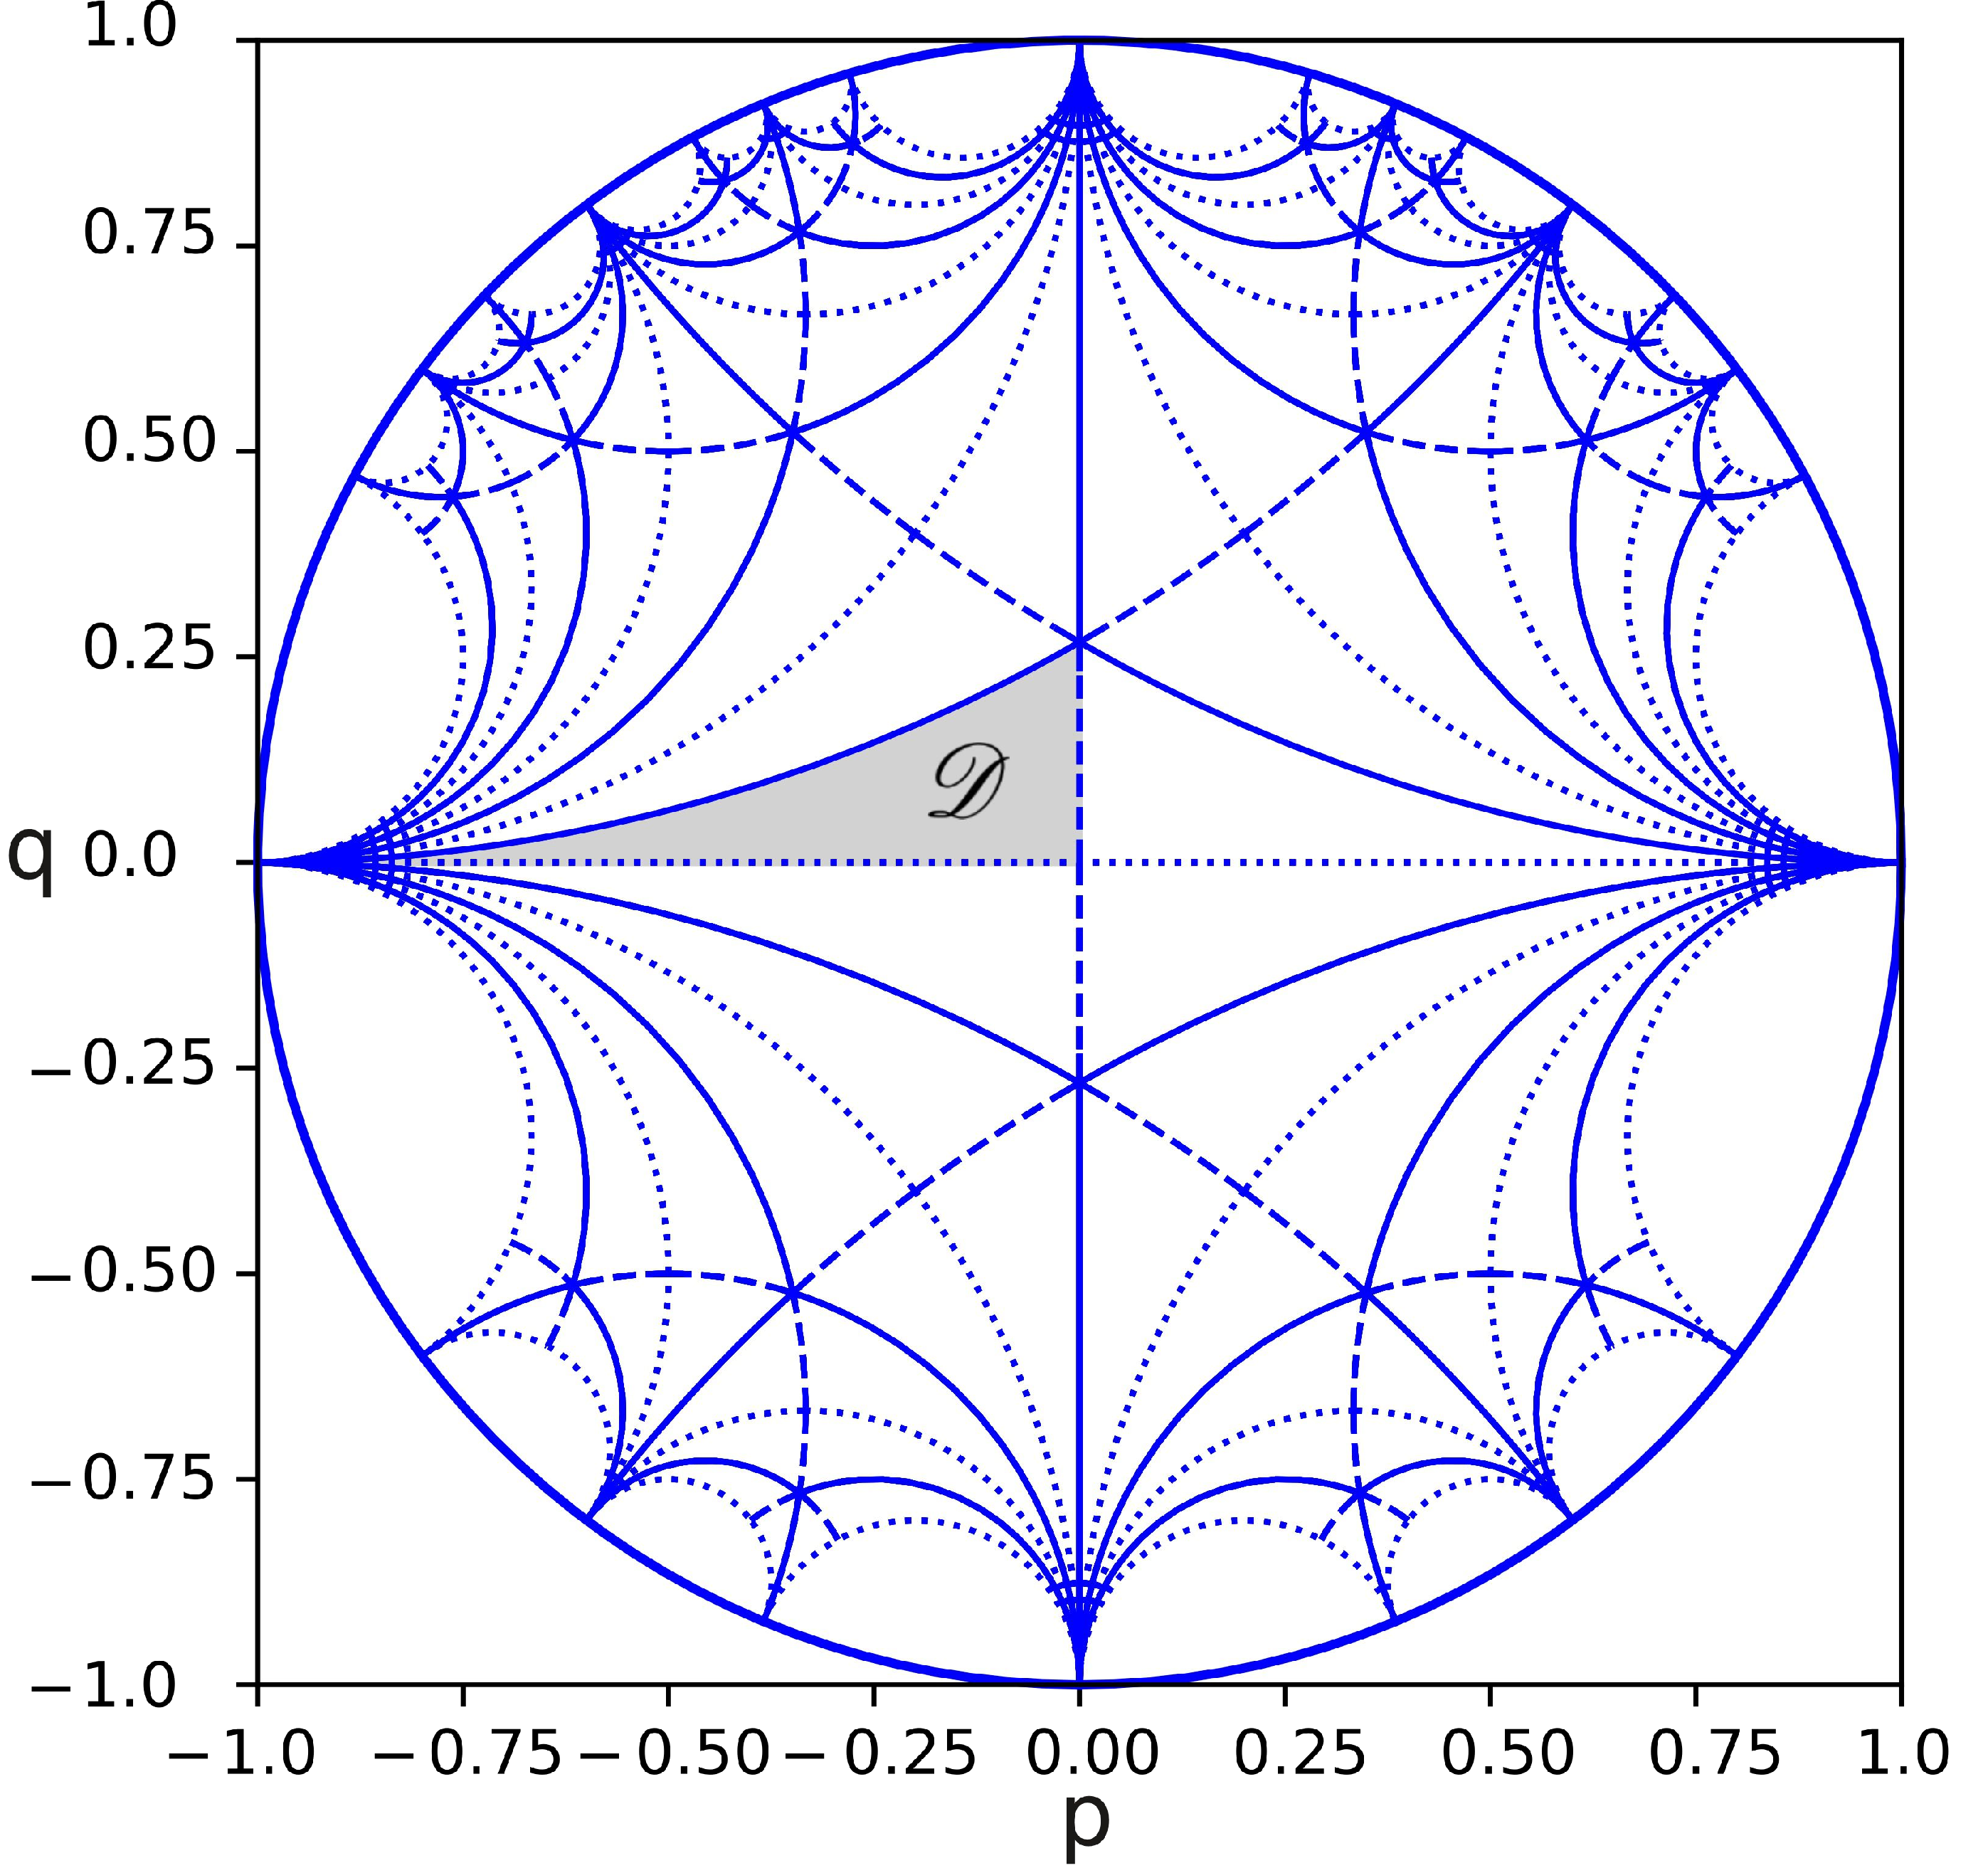
\includegraphics[scale=0.12]{./Figures/Fig1.pdf}
\caption{$GL(2, \mathbb{Z})$-induced tessellation of the configuration space of metric tensors $C_{11}, C_{22},C_{12}$  with $\det \mathbf{C}=1$ stereographically projected on the  Poincar\'e disk  $p^2 + q^2 < 1$ where 
$p = t(C_{11} - C_{22})/2$, 
$q = tC_{12}$, 
and  $t = 2/(2 + C_{11} + C_{22})$.
The highlighted domain $\mathscr{D}$  is the fundamental (minimal periodicity) domain.}
\label{fig:atlas0}
\end{figure}  
 


The presence of  the  energy barriers separating individual  energy wells makes the function $\phi(\mathbf{C})$ highly nonconvex, see Fig. \ref{fig:atlas1}. Therefore,  the corresponding  scale-free Landau model is  degenerate and needs to be regularized through the introduction of a cut-off length scale. This is   achieved in the MTM   by projecting the continuum problem on  a uniform mesoscale grid and associating the  periodic  elastic  energy   with   discrete   elements  whose linear size $h$ becomes a  physical parameter.  In this way the infinite dimensional space of continuum deformation fields is reduced to a finite dimensional set of compatible, piece-wise affine mappings, see  \cite{SM} for details. 

\begin{figure}[h!]
\begin{center}
%\subfigure[]{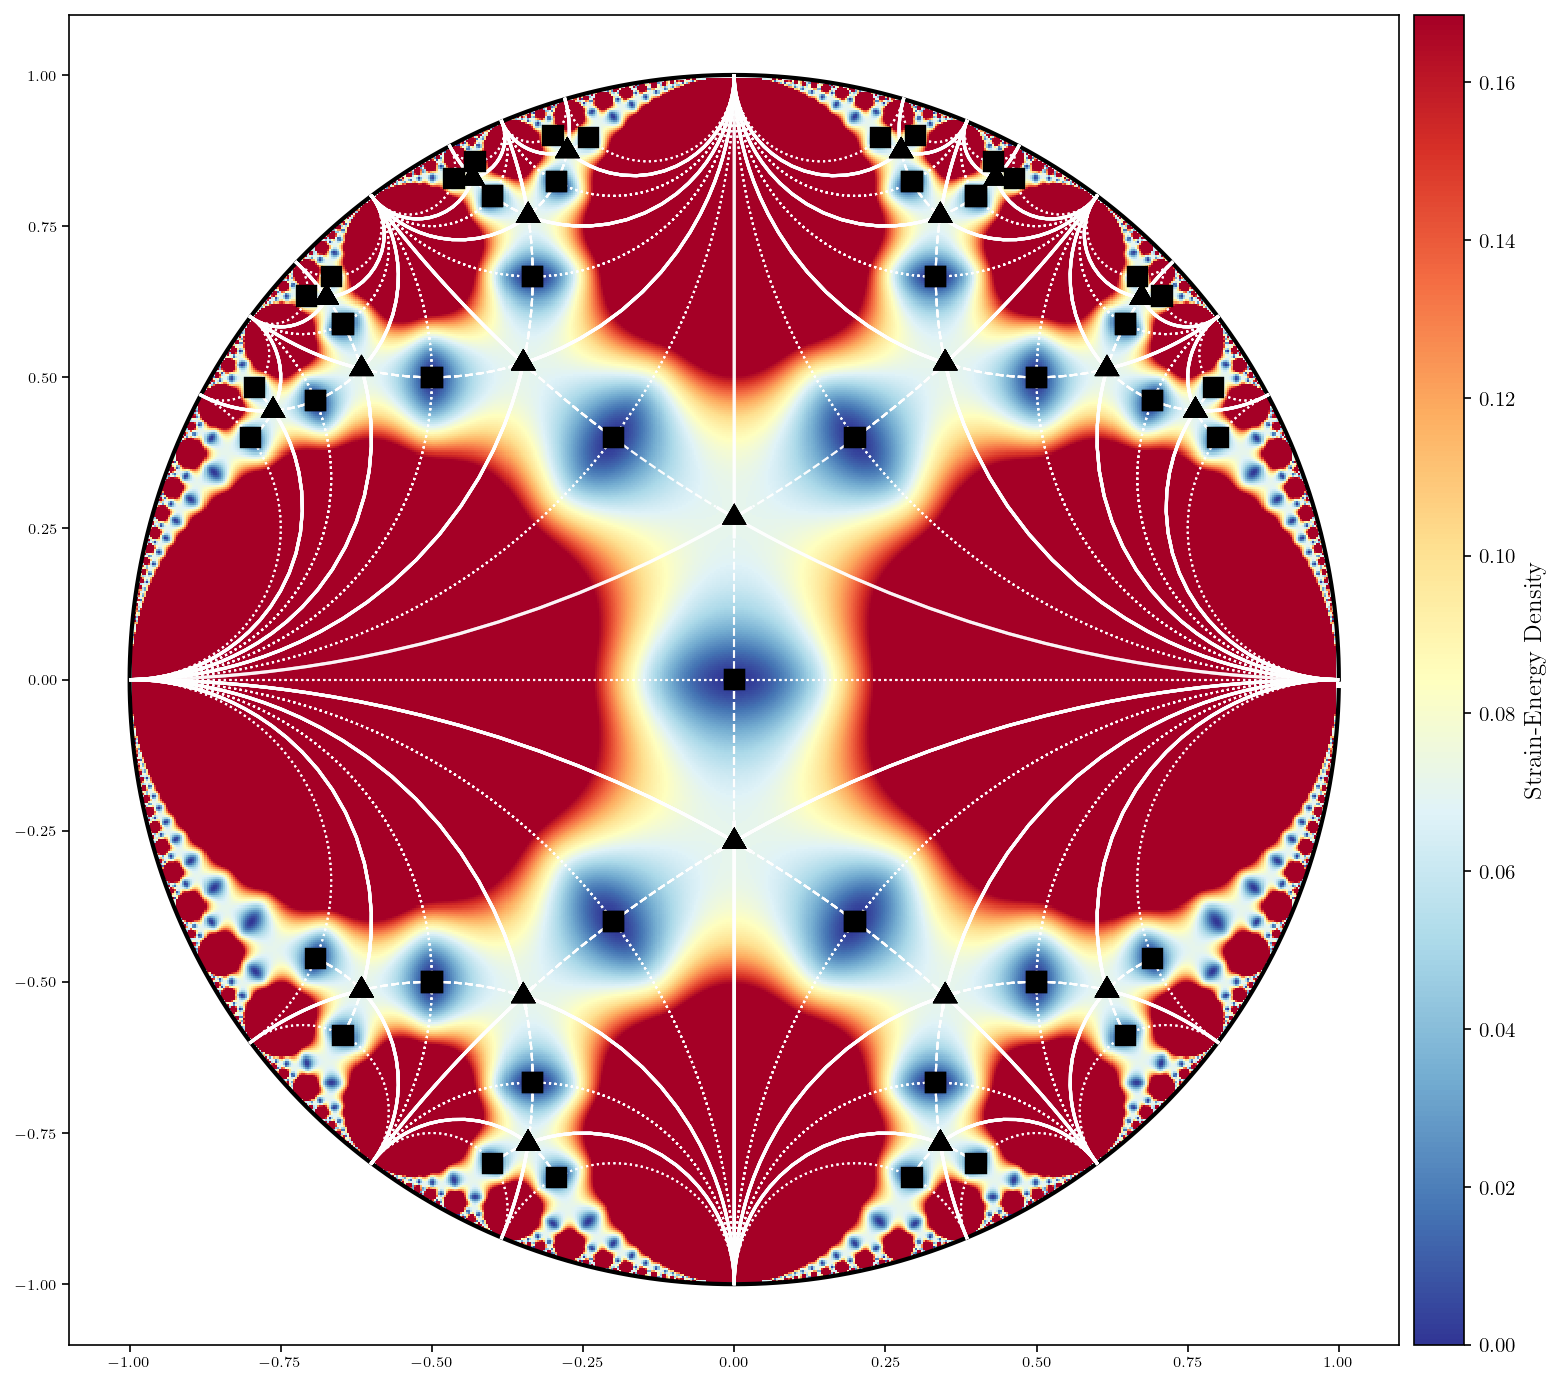
\includegraphics[scale=0.05 ]{figures_ordering/figure_02.png}}
%\hspace{0.5cm}
 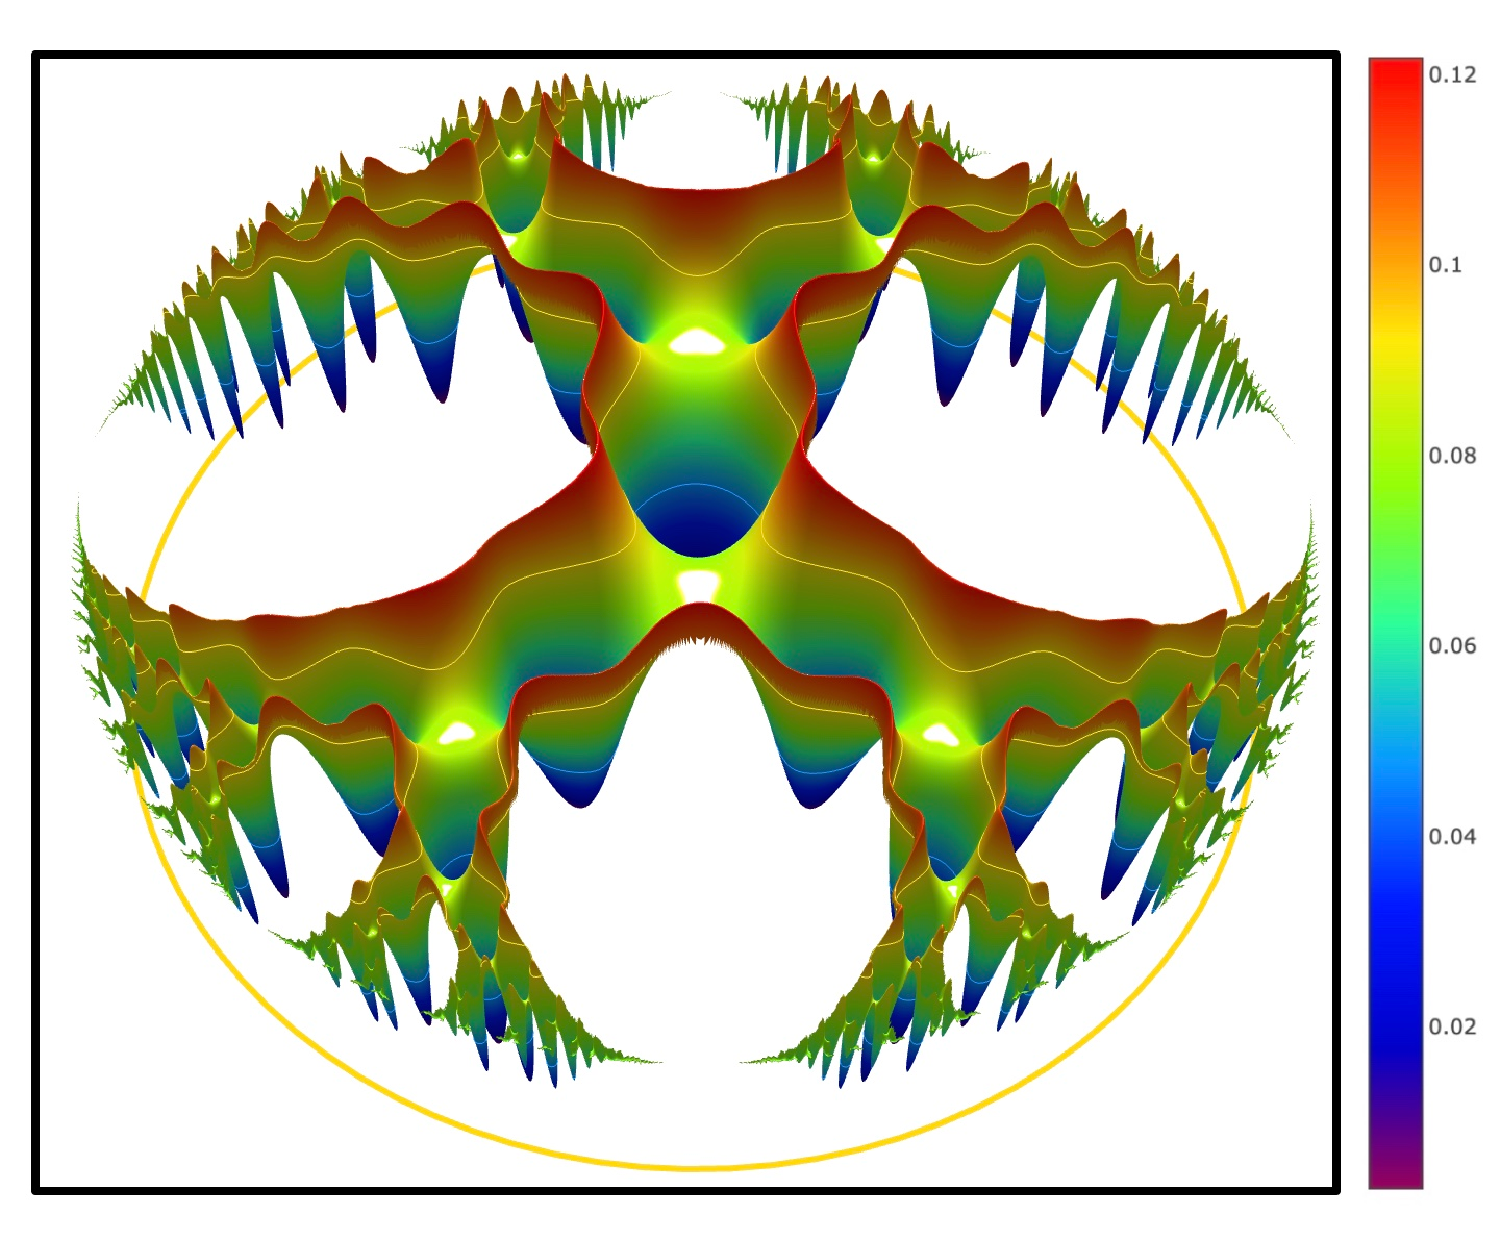
\includegraphics[scale=0.25]{./Figures/Fig2.pdf}
\end{center}
\caption{Energy landscape in the space of metric tensors (Poincar\'e) disk  shown in Fig. \ref{fig:atlas0}. Color indicates  the energy level with only the lowest energy levels shown. The deepest energy wells correspond to equivalent representations of the same square lattice.
%(a) Tessellated representation showing the discrete sampling of the strain-energy density field. (b) Corresponding continuous height plot of the strain-energy landscape over the same coordinate system.
}
\label{fig:atlas1}
\end{figure} 
 
The  driven system of this type will experience a rich repertoire of instabilities.   Specificaly,  an incremental elastic energy minimization of a system subjected to  quasistatic loading will generically lead to repeated jump discontinuities representing  branch switching events. The energy losses associated with such jumps will represent  plastic dissipation; in the continuum limit the jumps   will merge  giving rise to  rate-independent plasticity \cite{Puglisi2005-lg}.

\begin{figure}[ht!]
\centering
%\includegraphics[scale=.1]{figures_ordering/figure_073.pdf}
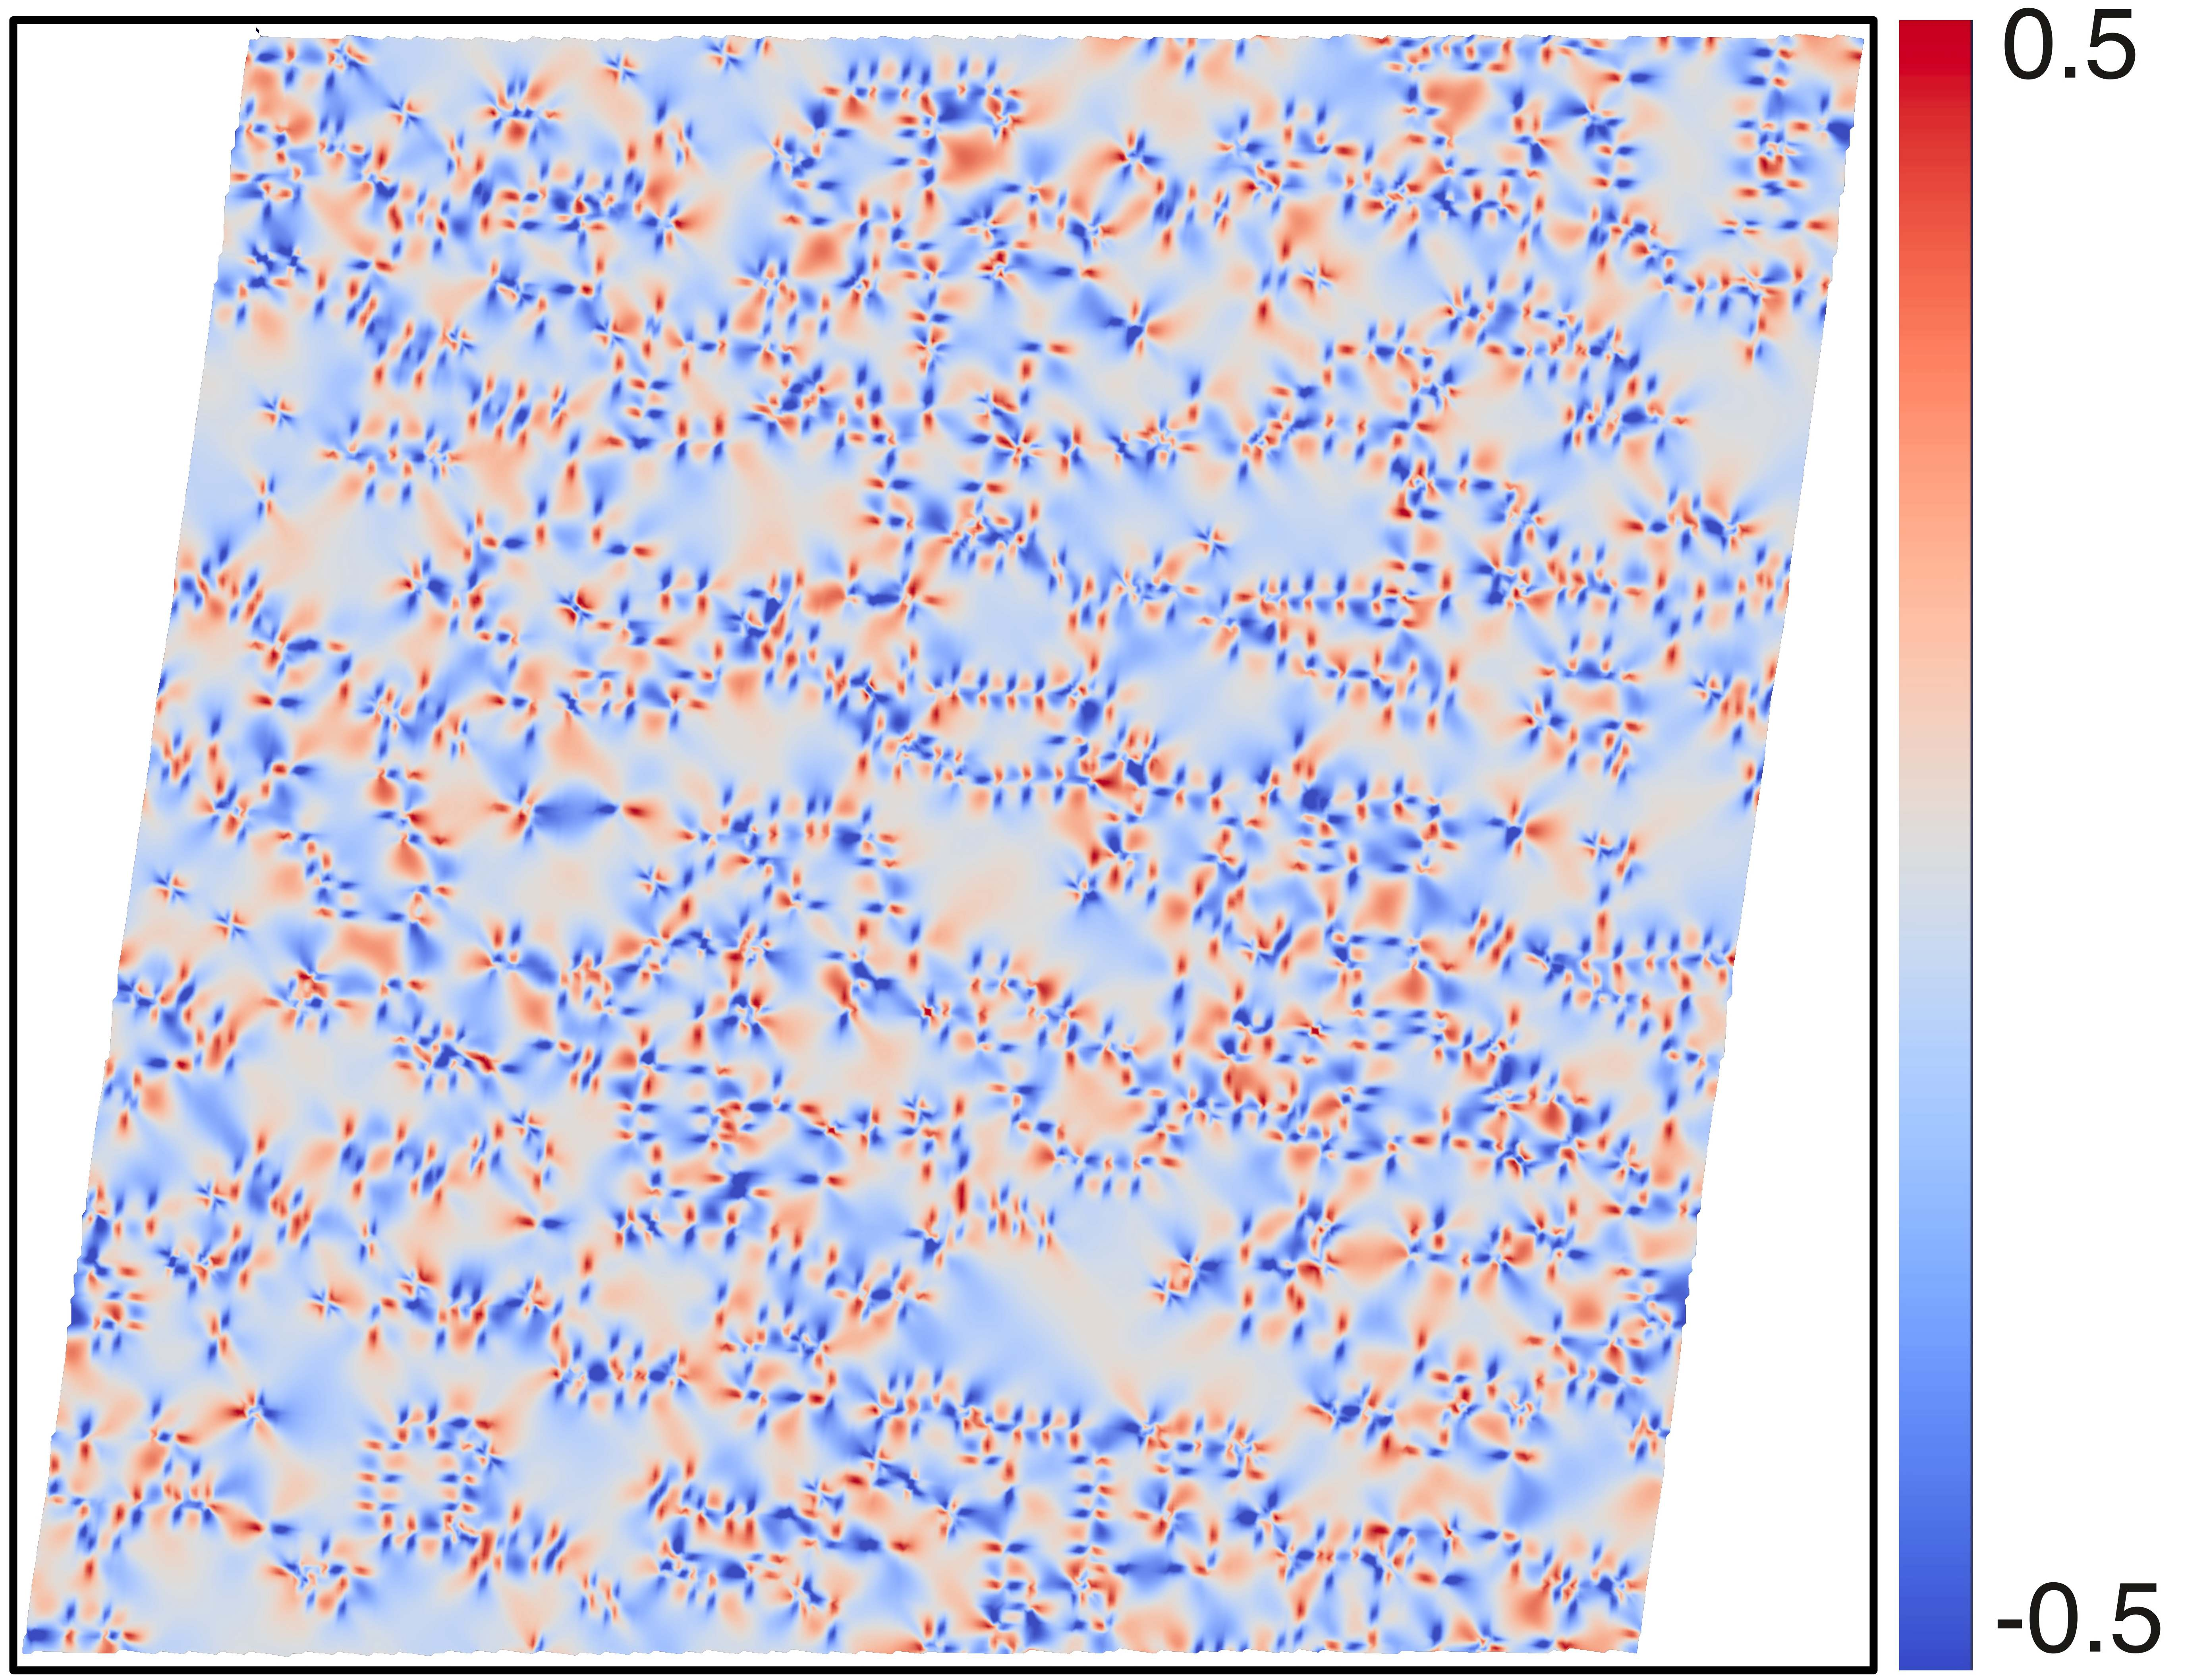
\includegraphics[scale=.055]{./Figures/Fig3.pdf}
\caption{Dislocated configuration emerging after a  homogeneous lattice is mechanically driven to the threshold of elastic instability. Colors indicate the level of the shear component of the Cauchy stress tensor $\sigma_{xy}$. The highest stress levels of both signs correspond to the location of dislocation cores. } 
\label{fig:22}
\end{figure}
 In our numerical experiments a square crystal  was represented by  $N\times N$ nodes,  with $N=400$. The nodes were arranged into  triangular finite elements.  We loaded the corresponding athermal  system quasi-statically by  applying the affine displacement field 
 \begin{equation}
  {\bf u}(\alpha,{\bf x})= (\bar{\bf F}(\alpha )-\mathbb{1}){\bf x} , 
  \end{equation}
 with 
 $$\bar{\bf F}(\alpha)={\bf I}+\alpha {\bf e}_1 \otimes  {\bf e}_2,$$
%${\bf F}(\alpha,\theta)={\bf I}+\alpha {\bf R}(\theta){\bf e}_1 \otimes{\bf e}_2$,
 where $ {\bf e}_ i$, $i=1,2$,  is the orthonormal basis of the reference square lattice.  In this way we imposed  simple shear along one of the principal slip directions with shear amplitude $\alpha$ serving as the loading parameter. By changing this parameter in strain increments of order $10^{-6}$, we advanced the loading. After each such increment the displacement field was updated by the energy minimization algorithm. Details of the discretization, of the  incremental  energy minimization algorithm and of  the implementation of the loading protocol under periodic  boundary conditions can be found  in \cite{SM}.  


  
\begin{figure}[h!]
\centering
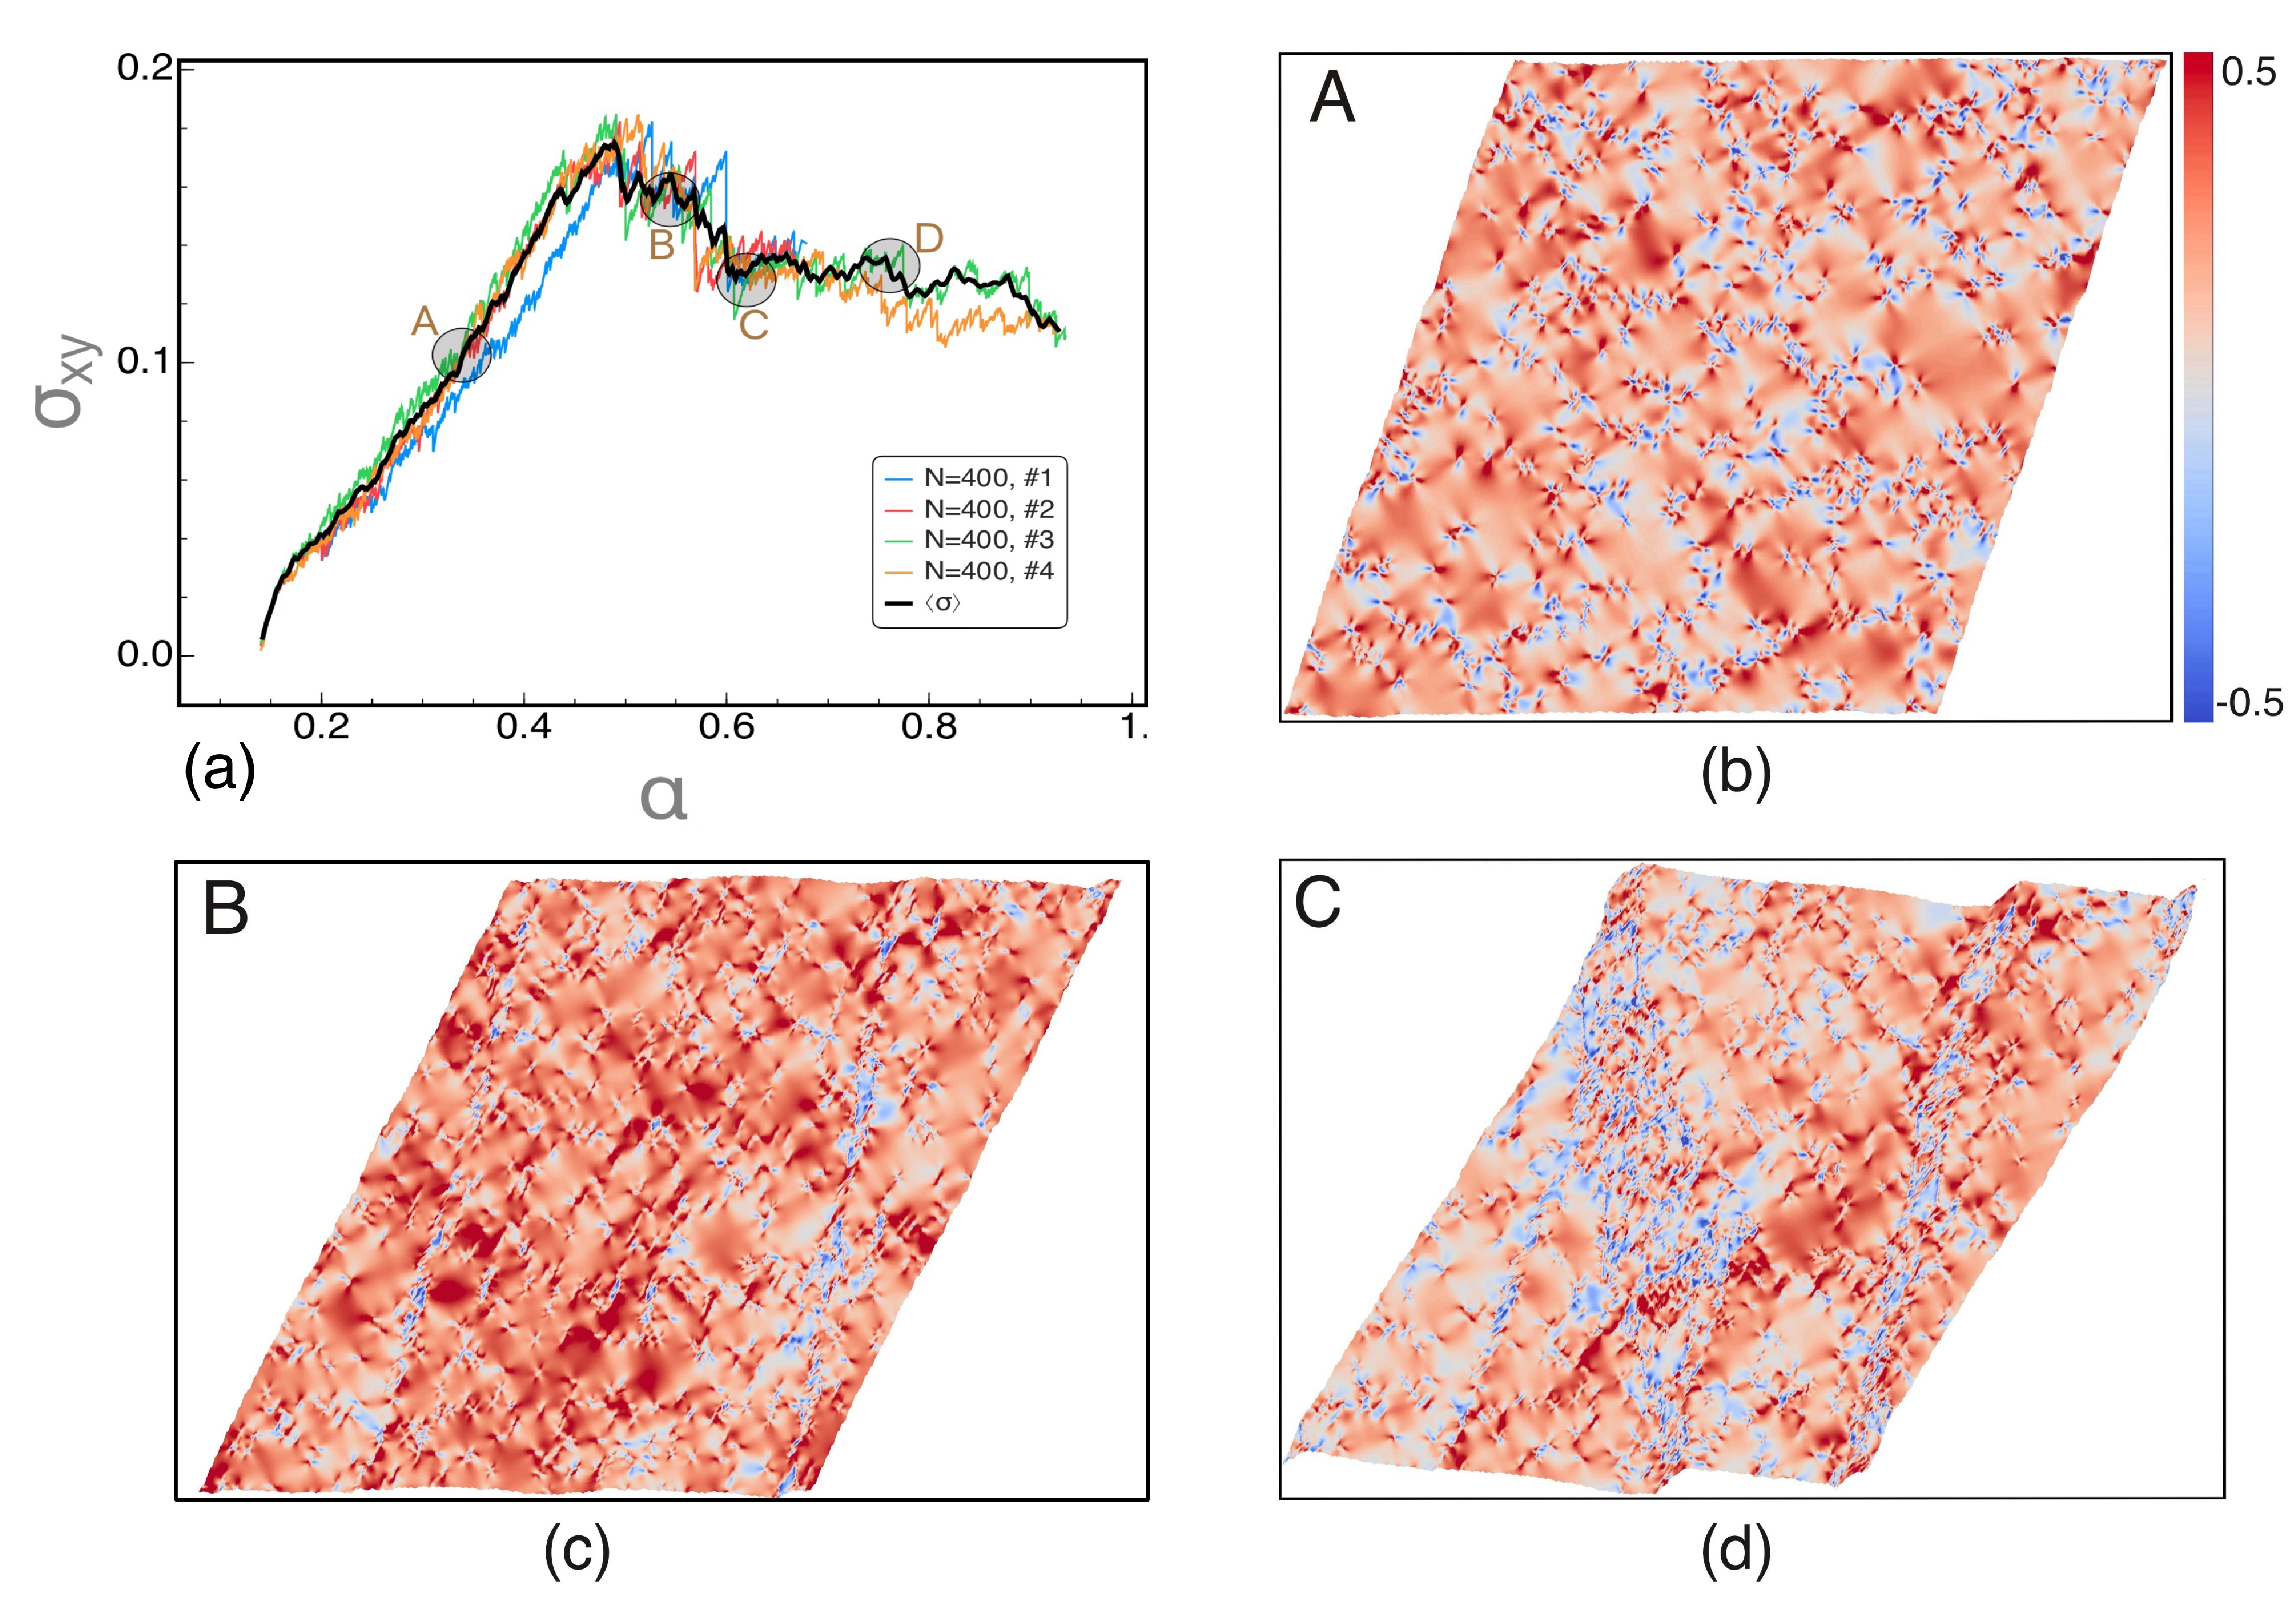
\includegraphics[scale=.11]{./Figures/Fig4.pdf}
\caption{(a) Stress-strain response of a quasi-amorphous crystal shown in Fig. \ref{fig:22}. (b) Dislocated configuration   in a typical pre-yield state characterizing  the stage of 'microplasticity'.  (c,d) Dislocated configuration characterizing  different stages of   unfolding of the quasi-brittle system size event.
 Colors indicate the level of the shear component of the Cauchy stress tensor $\sigma_{xy}$. 
%The hardening stage from $D$ to $F$ shows the pre-(second) yield 'microplastic' deformation. The transition from $F$ to $H$ correspond to a cluster of system spanning avalanches. The post-(second) yield stationary plasticity regime is represented by the state $I$ on a stress plateau.
}
\label{fig:2}
\end{figure} 
To obtain   a 'generic' sample, we first loaded a pristine (defect-free) crystal till the affine configuration  became elastically unstable. The corresponding  critical value of the loading parameter $\alpha=\alpha_c\approx0.138$ is very close to the threshold of   positive definiteness of the acoustic tensor \cite{Simpson1989,Grabovsky2013,Steigmann2023}, see  the explicit formulas in \cite{SM}. The breakdown of an elastic state takes the form of a major system-size inelastic event. It leads to multiple nucleation of dislocations which  apparently transforms a perfect crystal into a  quasi-amorphous system, see Fig.~\ref{fig:22}.  We observe that the  unfolding  of the elastic instability  is  arrested at a  state which one can expect to be only marginally stable. 
 
 
%\emph{Mechanical response. }

  
We continued to load the obtained  'generic' sample using the same athermal quasistatic  protocol and the ensuing stress-strain response   is shown  in Fig.~\ref{fig:2}(a). Its salient feature is the presence of irregularly placed elastic branches interrupted by intermittent stress drops; the latter represent  plastic avalanches  involving  partial  unlocking of dislocation structures.  Among  these avalanche-type events, one major stress drop stands out and can be interpreted as a plastic  yield separating  two different regimes. While the first (pre-yield) regime is characterized by quasi-elastic hardening, the second (post-yield) regime is  represented by a stress plateau which suggests quasi-stationary plastic flow, see Fig.~\ref{fig:2}(a). 




Our  Fig.~\ref{fig:2}(b) illustrates  the stress field in a typical pre-yield state $A$.  The restructuring of the dislocation pattern  is relatively minor with dislocations moving only between the  preexisting locking sites, cf.  Fig. \ref{fig:22}. Such    response  is known to be a characteristic  pre-yield feature  for  both amorphous  and (defective) crystalline  solids \cite{Maas2018-qu,Papanikolaou2017-ld,Sparks2018-zp,sparks2019avalanche,Rizzardi2022-iz,Duan2023-ue}. This  'microplasticity' regime ends with the system-size event reminiscent of  quasi-brittle plastic yield encountered in  well-annealed glasses and  also in some sub-micron crystals \cite{bei2008effects,chrobak2011deconfinement,wang2012pristine,Cui2017-xn,Greer2011-hi,Brenner1956-rx,Brenner1958-dr,Sharma2018-iw,Mordehai2018-qm,Lilleodden2006-jq,Corcoran1997-vt}.  As we see from  Fig.~\ref{fig:2}(a) it takes the form of a two-stage transition $A \to B \to C$; the snapshots of the spatial  stress  configurations in the states $B$ and $C$ are shown in  Fig.~\ref{fig:2}(c,d).  The  associated  global restructuring reveals collective dislocation activity manifested through  the emergence of  system-spanning shear bands.  

 Additional   details can be seen in Fig.~\ref{grains3} where we illustrate the strain-energy density field in the state $C$. We see  the development of  low-energy rotated patches of the original lattice forming intricate polycrystalline grain texture with  misorientation of neighboring grains  controlled by the overall compatibility of the deformation field as explained in   \cite{Baggio2023-qu}; the elastic energy is localized around  dislocation-rich grain boundaries.  In the inset in Fig.~\ref{grains3}  we made  dislocations of different sign clearly visible: they were identified via Delaunay triangulation and   nodes with five/seven  neighbors  are shown in blue/red.  One can see    the emergence of energy minimizing structure of grain boundaries \cite{Sutton1984-us,Priester2012-wx,Randle2024-tf} with  ubiquitous presence  of   $\Sigma 5$ grain boundaries, see  \cite{Baggio2023-qu} for the explanation. 
% and dislocations correspond to adjacent pairs where the ordering 5-7 or 7-5 determines the sign).
\begin{figure}[h!]
\includegraphics[scale=.025]{./Figures/Fig5.pdf}
\caption{The micro-configuration  configuration corresponding to the state $C$ marked  in Fig. \ref{fig:2}. Colors indicate the magnitude of strain-energy  density. The inset shows a single grain and details the dislocation structure of the grain boundaries. }
\label{grains3}
\end{figure}

 % It also shows  that the shift from 'local' to 'global' dislocation rearrangements leads to
  
  

% In other words, dislocations appear to be confined inside the effective cages where they can pile up but from where they can only rarely escape by breaking the existing locks.

 
%\begin{figure}[h!]
%%\includegraphics[scale=.1]{figures_ordering/figure_11.pdf}
%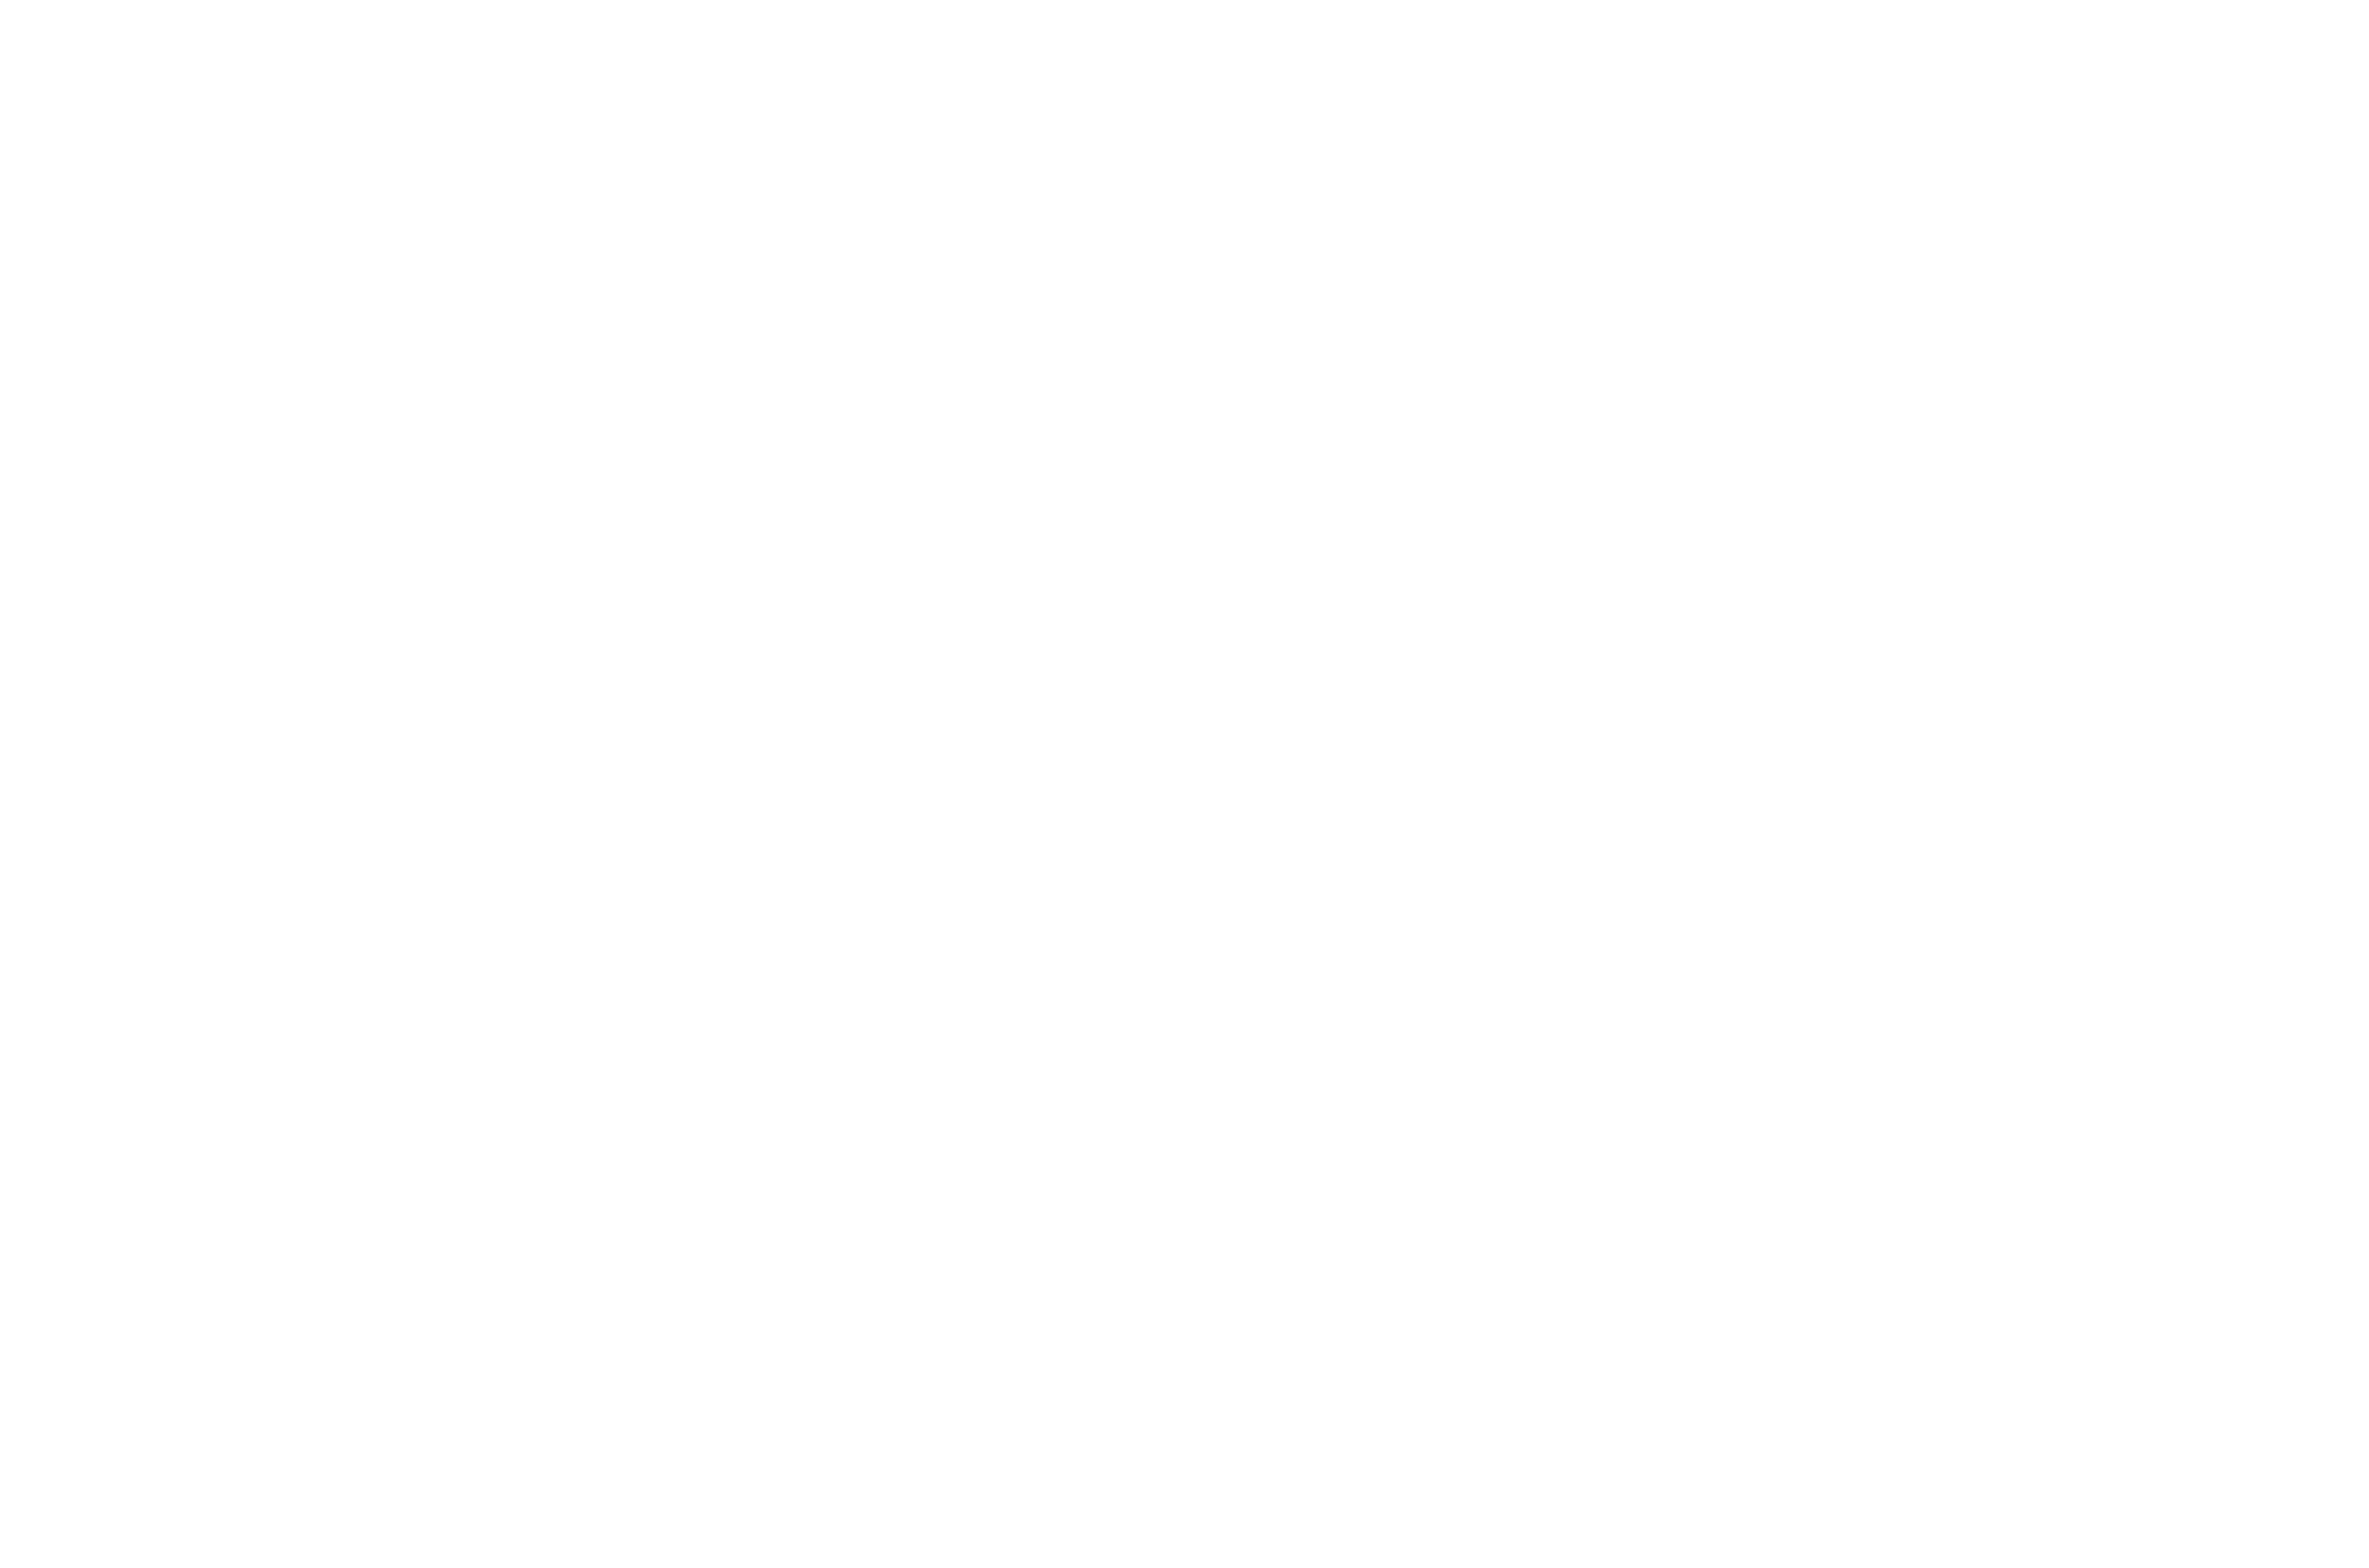
\includegraphics[scale=.053]{./Figures_ordered/Fig5.pdf}
%\caption{ Dislocated configuration   in a typical pre-yield state characterizing  the stage of 'microplasticity'. The state $A$  is marked  in Fig. \ref{fig:2}. Colors indicate the level of the shear component of the Cauchy stress tensor $\sigma_{xy}$.}
%\label{fig:031}
%\end{figure}




%It is natural to interpret the  regime-separating  system-size event  as a quasi-brittle plastic yield.
 

%  \begin{figure}[h!]
%\centering
%\subfigure[]{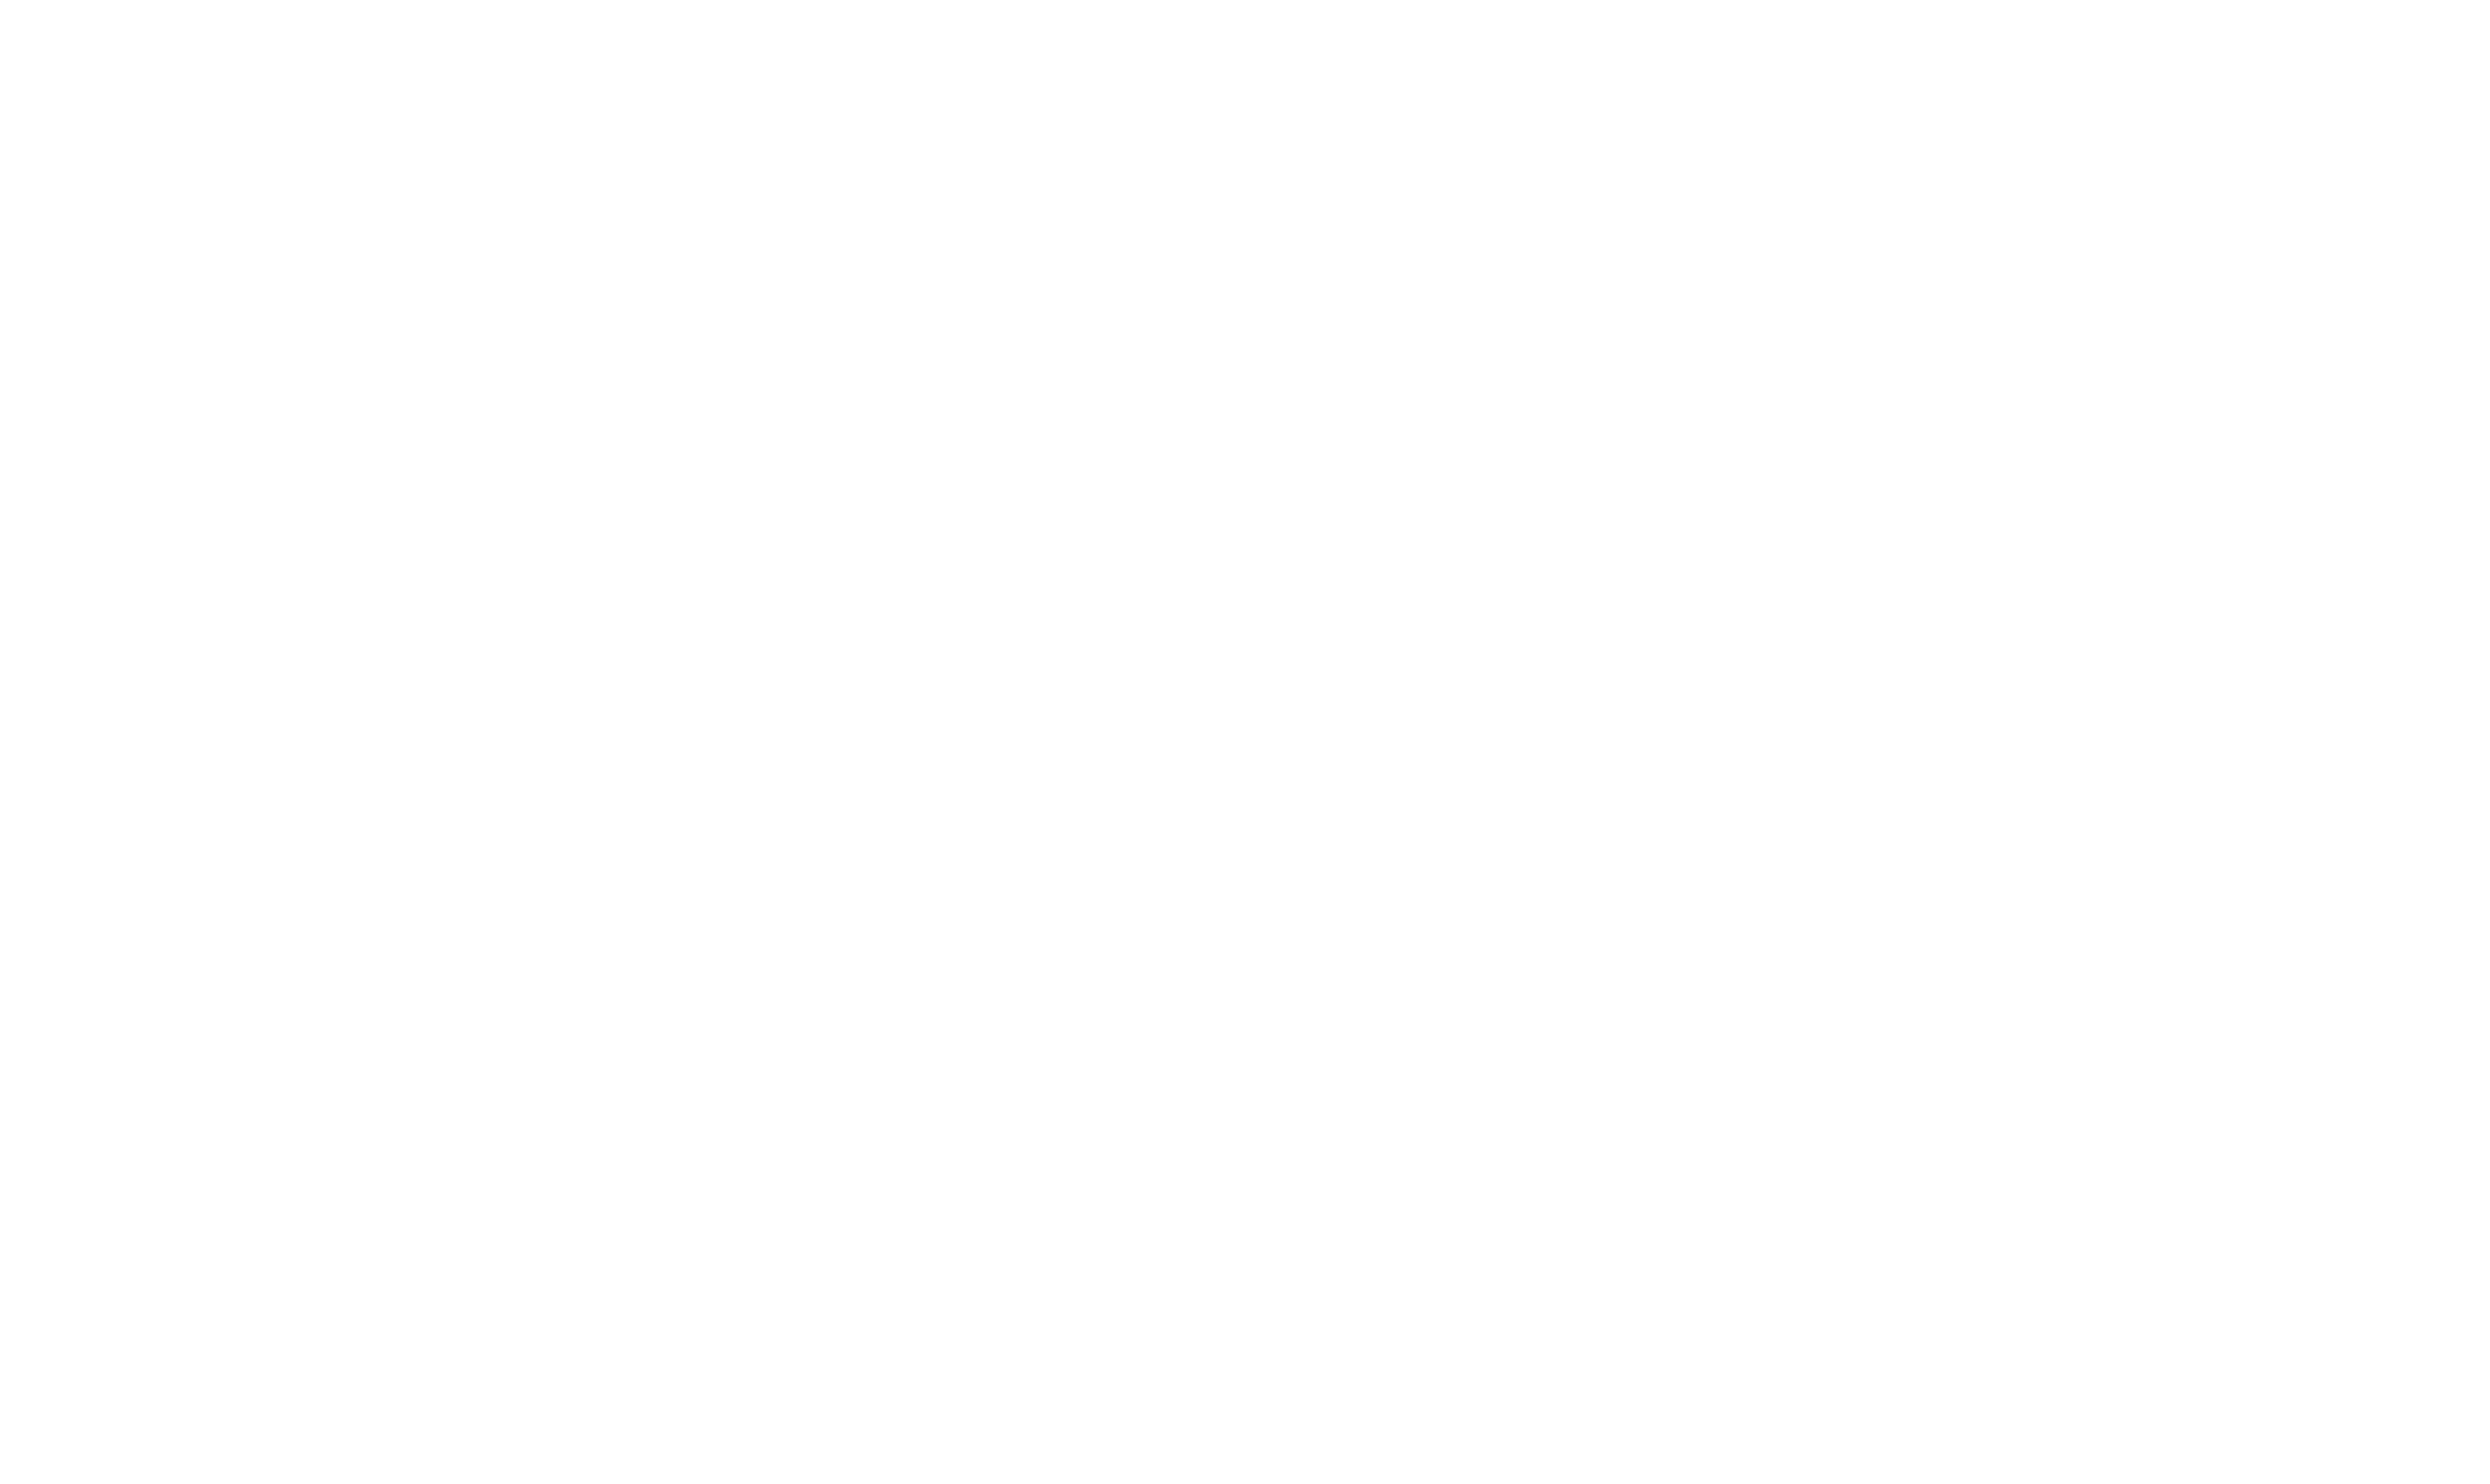
\includegraphics[scale=.0371]{./Figures_ordered/Fig6-a.pdf}\label{fig:03a}}
%\subfigure[]{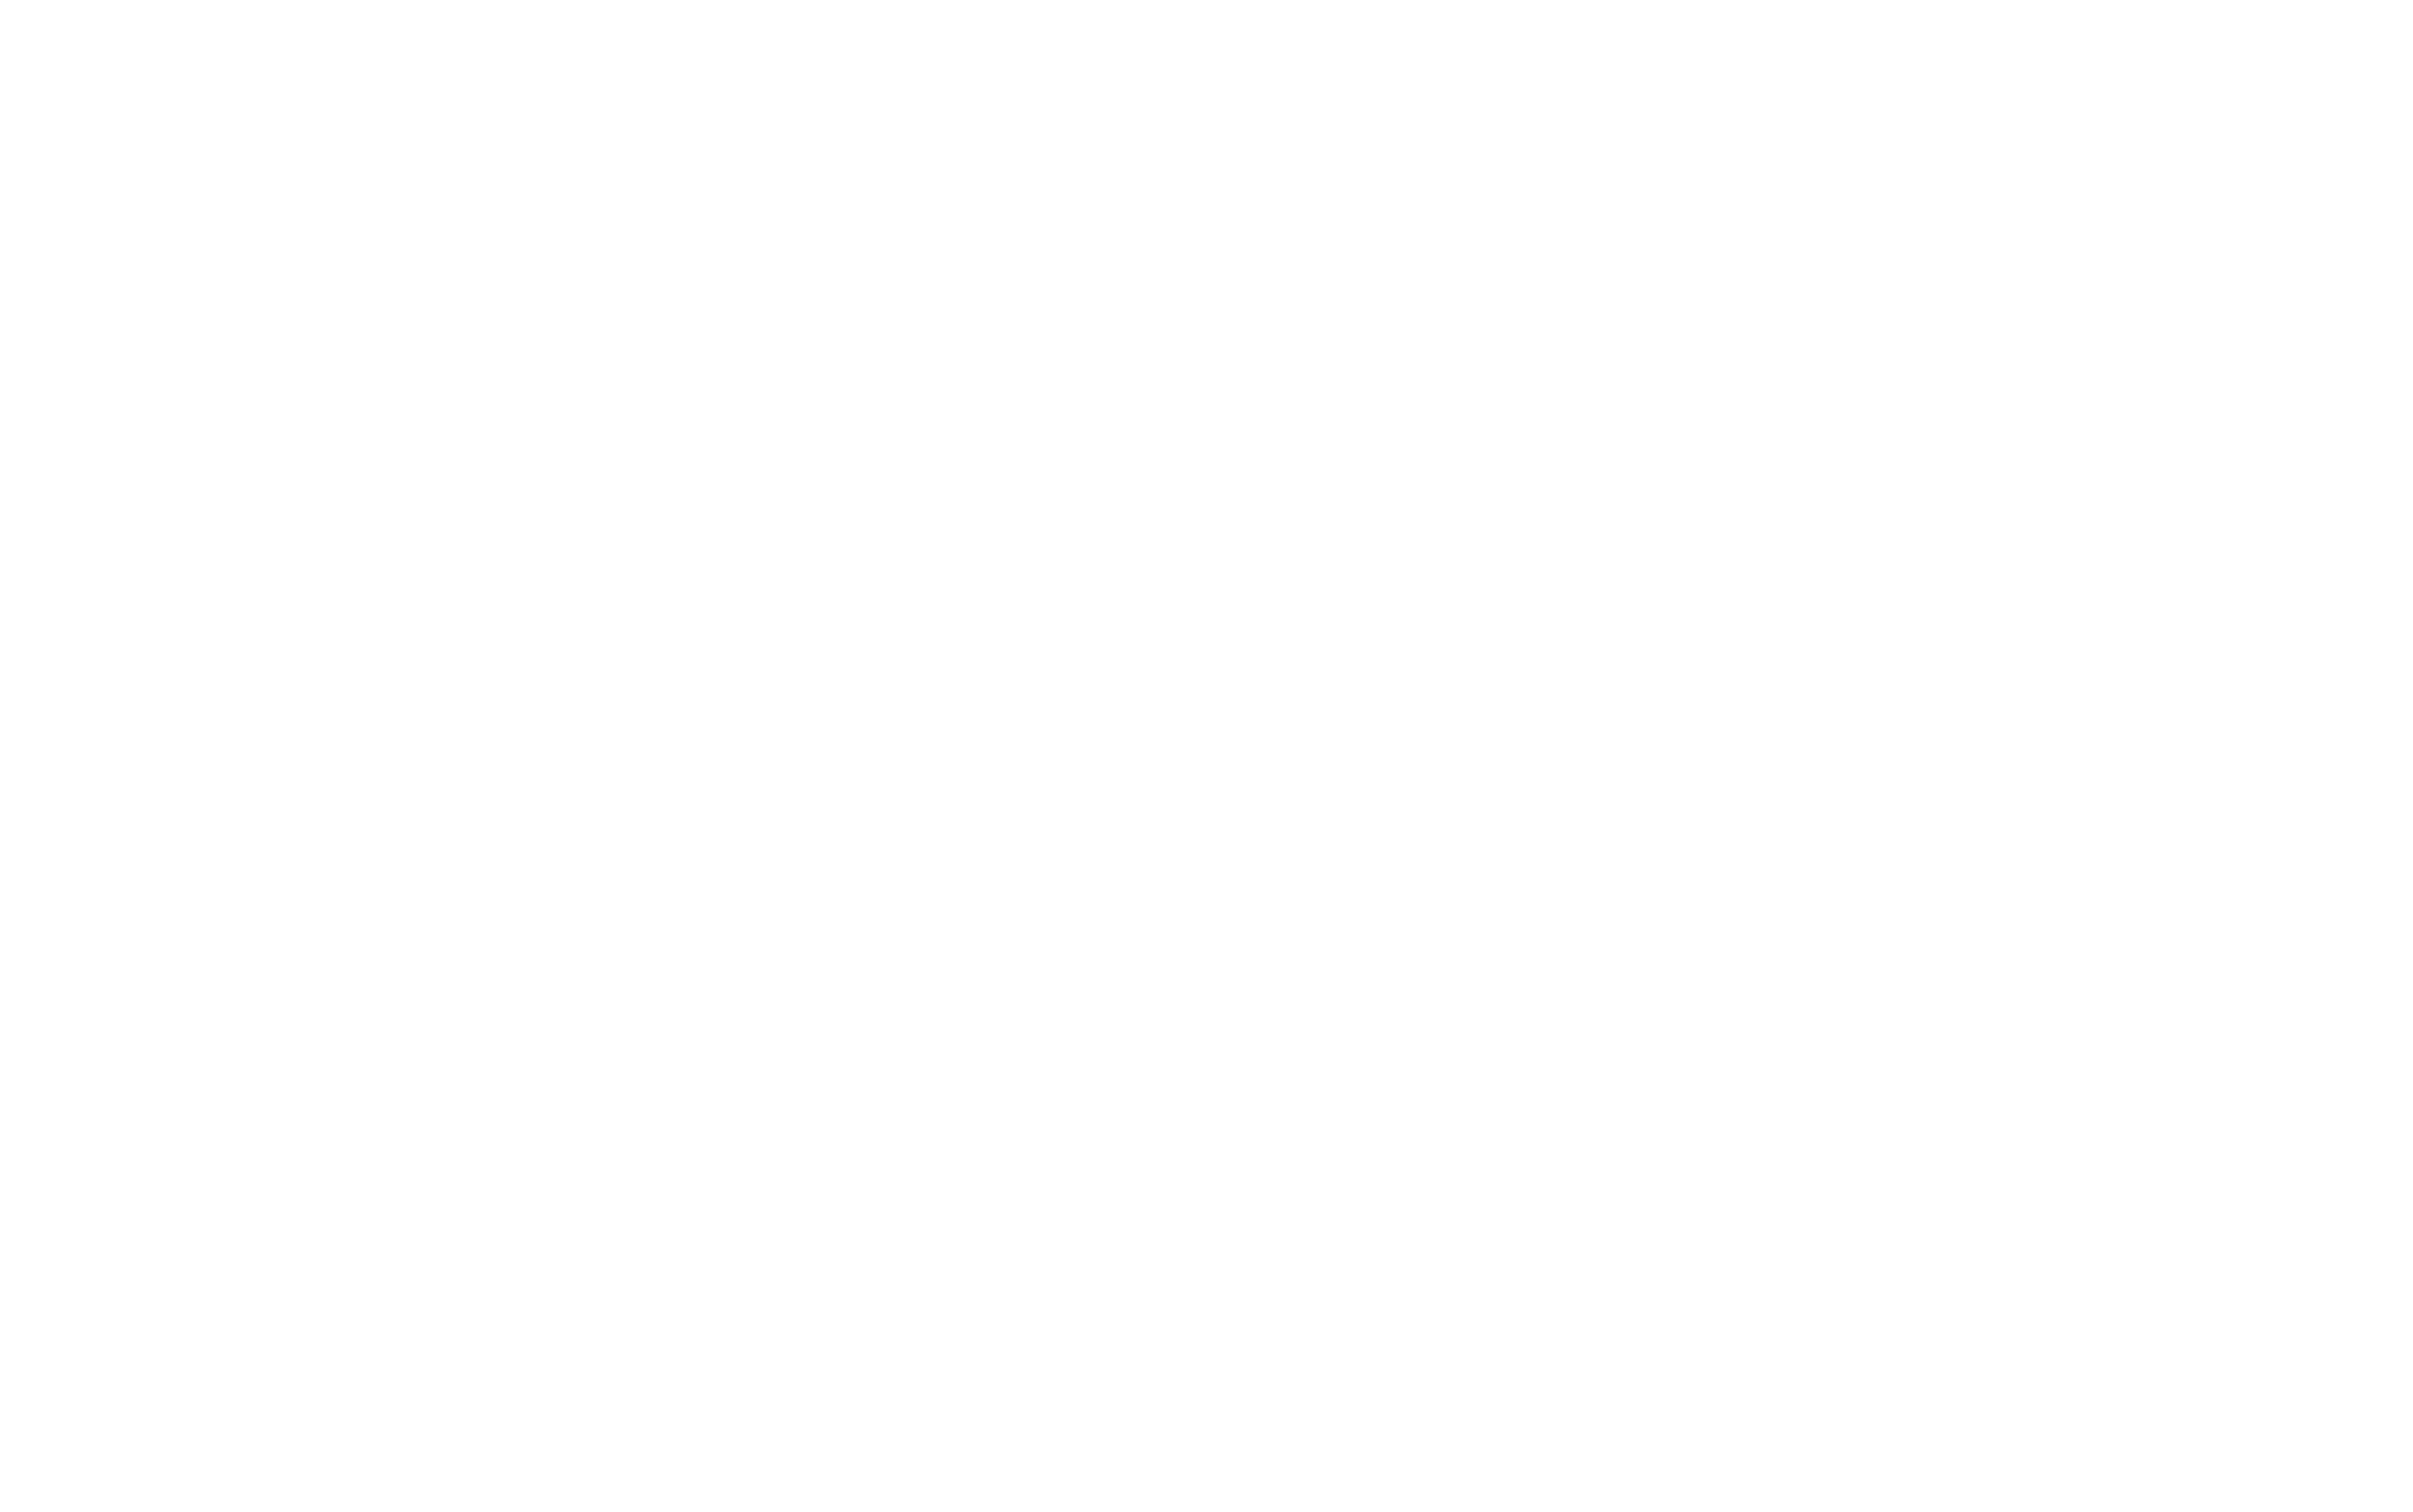
\includegraphics[scale=.0371]{./Figures_ordered/Fig6-b.pdf}\label{fig:03b}}
%\caption{Dislocated configuration characterizing  different stages of   unfolding of the quasi-brittle system size event. The states $B$ and $C$ are marked  in Fig. \ref{fig:2}. 
%Colors indicate the level of the shear component of the Cauchy stress tensor $\sigma_{xy}$.
%} \label{fig:03}
%\end{figure}


The post-yield regime, characterized by relative stabilization of the average stress level, can be interpreted as a quasi-stationary non-equilibrium steady state (NESS). A representative snapshot of the micro-configuration of the crystal in the state $D$ is shown in Fig.~\ref{fig:04} where we see further development of the polycrystalline grain texture. During  intermittent avalanches characterizing this regime  larger  grains occasionally merge  while small grains continue to emerge. In this way the   self-organization of dislocations  continues to generate  additional scales which contribute to the  formation of the global hierarchical structure.  Through  the  transitions from isolated dislocation motion to collective dislocation behavior  the system  acquires access to a much broader repertoire of  relaxation mechanisms. A detailed analysis of the avalanche structure shows that while in the pre-yield regime plastification takes place  primarily in the form of isolated, linear arrangements of transformed elements,  a typical post-yield avalanche reveals extended plastified regions with complex branching. \textcolor{blue}{This structural evolution is vividly reflected in the corresponding Poincaré configurational space representations (Fig.~\ref{fig:conf_space}). During the pre-yield micro-plastic regime, the system predominantly explores a limited set of energy wells---mostly three---corresponding to fundamental dislocation gliding along the $x$ and $y$ directions (Fig.~\ref{fig:conf_space}(a)). Conversely, in the mature post-yield regime, the emergence of system-spanning shear bands and the massive accumulation of plastic deformation drive the system to access a much richer repertoire of lattice orientations, leading to a sprawling population across many more equivalent energy wells, see Fig.~\ref{fig:conf_space}(b).}

\begin{figure}[h!]
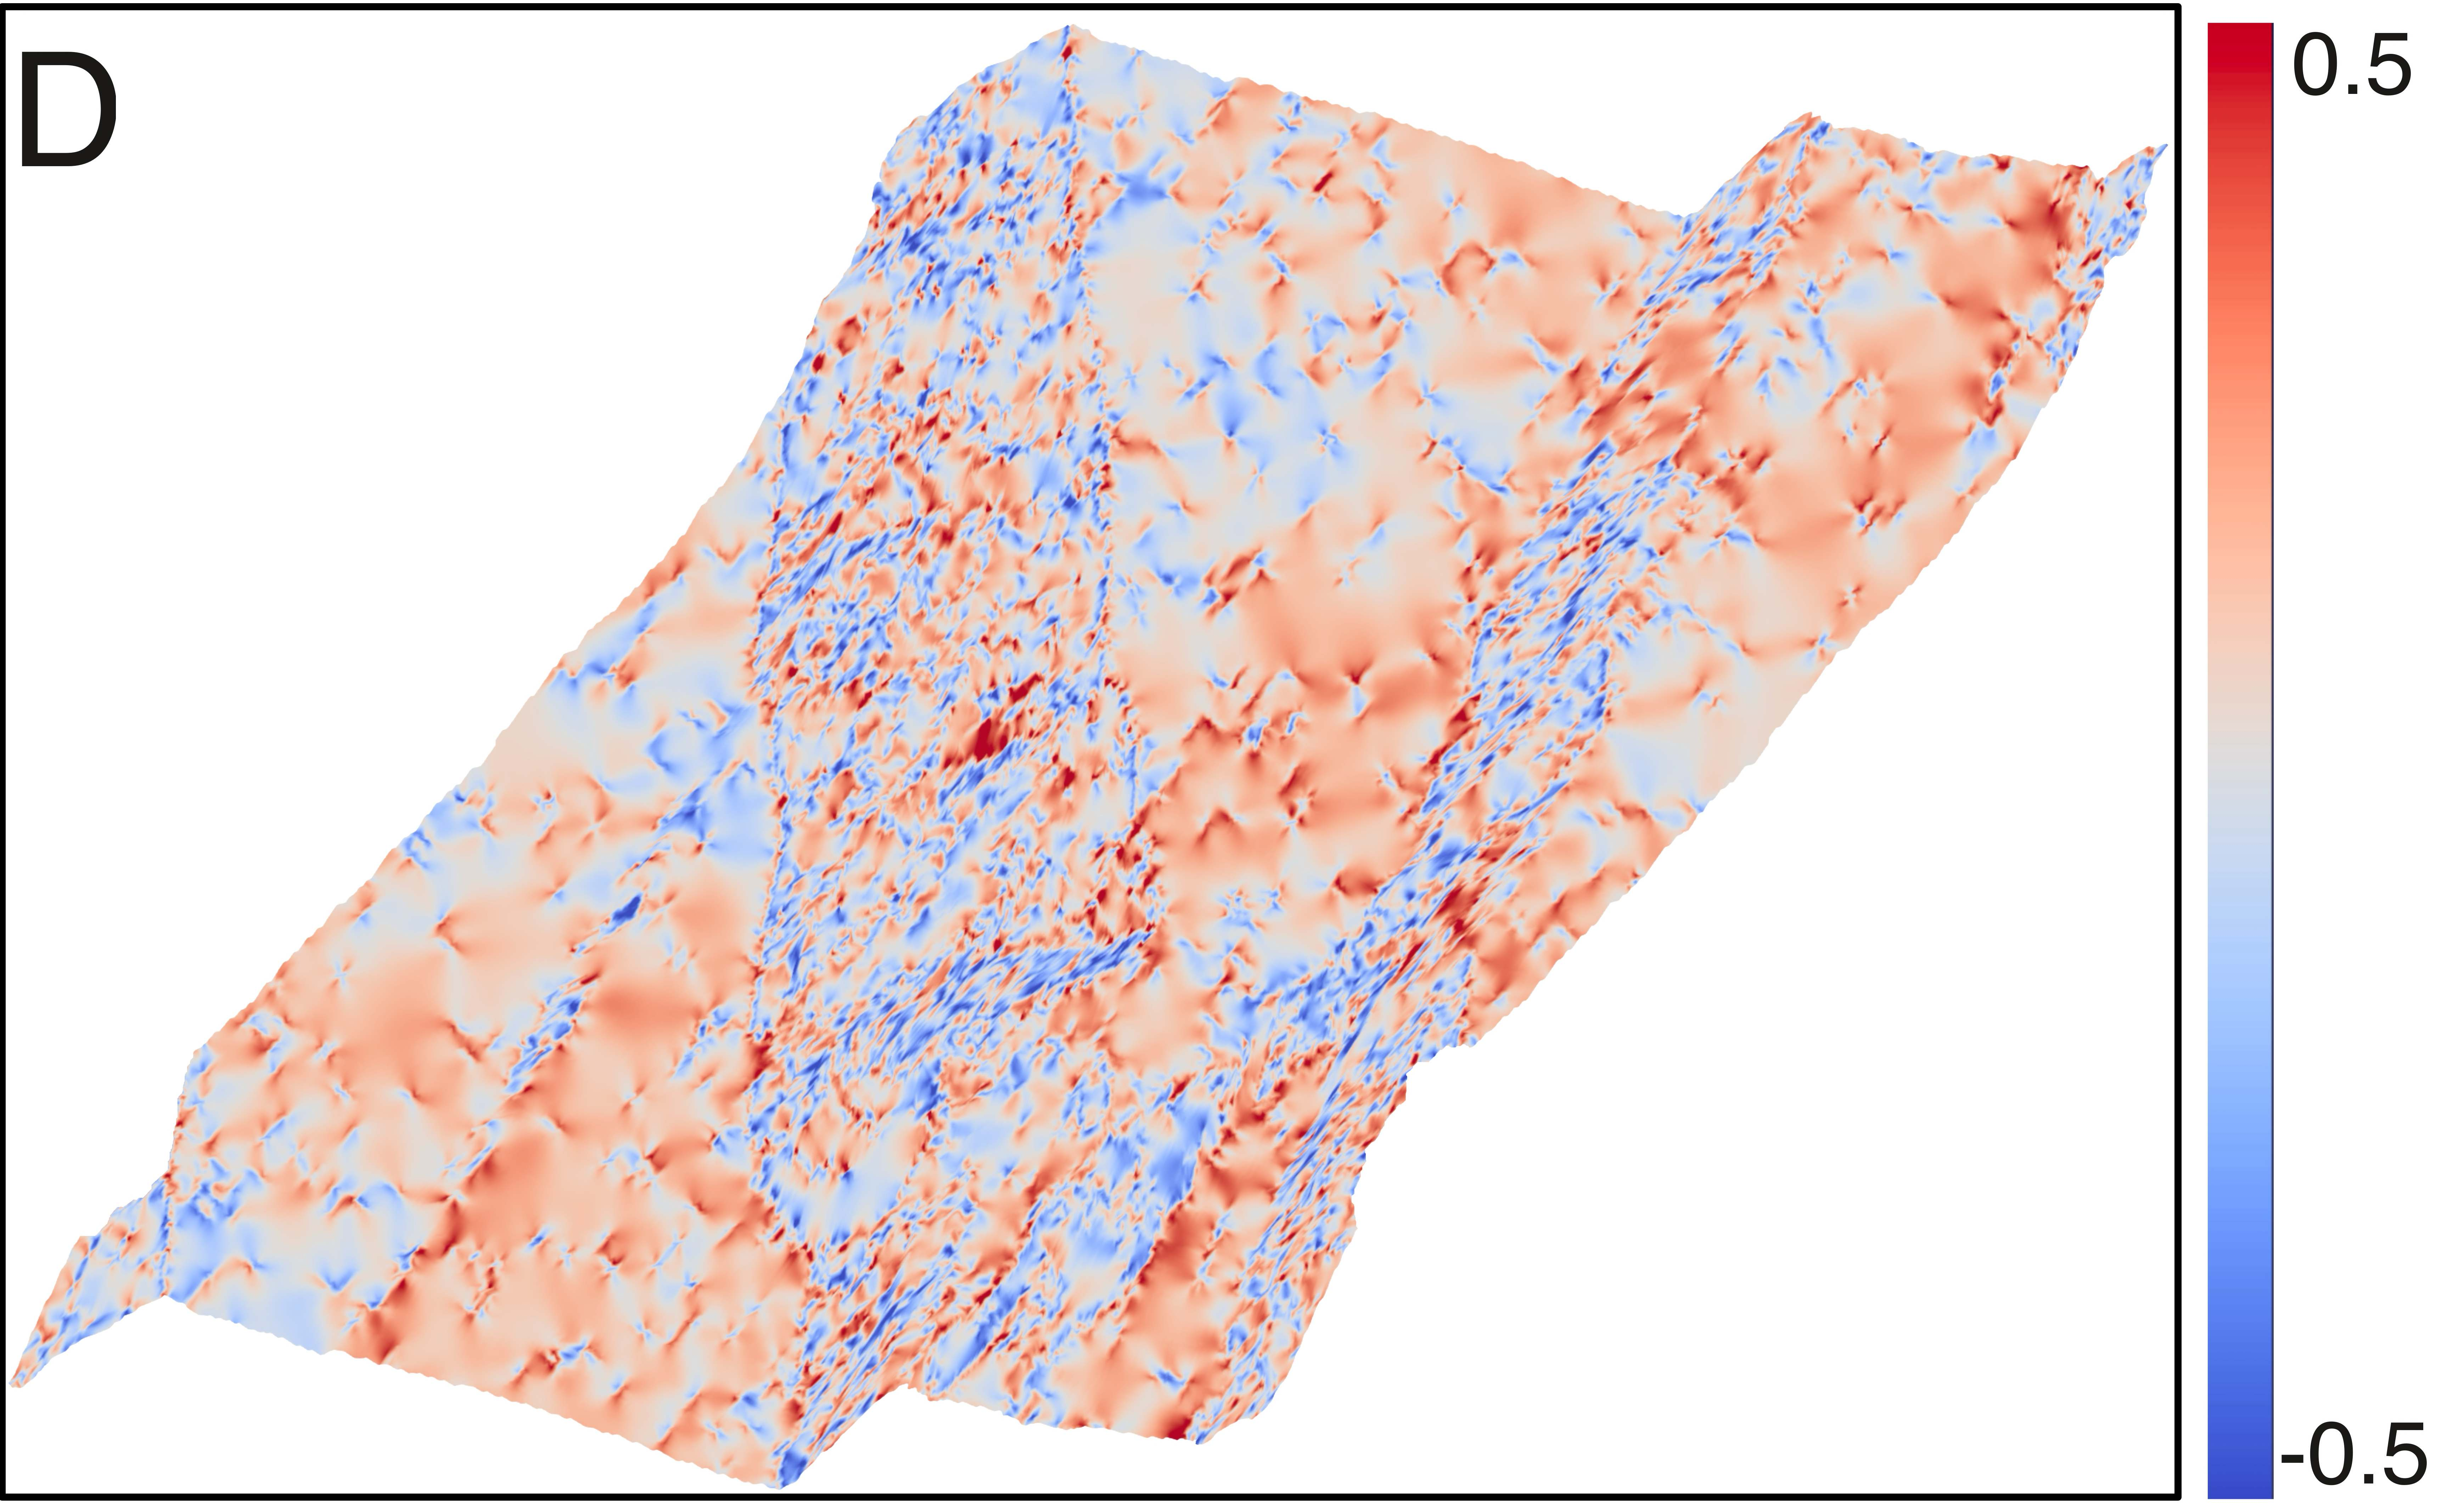
\includegraphics[scale=.05]{./Figures/Fig6.pdf}
\caption{Mature shear bands in the regime of stationary post-yield plastic flow represented by the state $D$ marked  in Fig. \ref{fig:2}.   Colors indicate the level of the shear component of the Cauchy stress tensor $\sigma_{xy}$.
}
\label{fig:04}
\end{figure}


An important window into  the  micro-mechanics  of solids  undergoing plastic flow is provided by the study of the statistical structure  of plastic fluctuations \cite{Papanikolaou2017-ld,Weiss2015-eh,Zaiser2006-gk,Tarp2014-ro,Miguel2006-wd,Alava2014,Sethna2017}.  Thus, it is known that in amorphous solids the probability distribution of the energy drops associated with individual avalanches $\Delta W = W_{\text{before}} - W_{\text{after}}$, where $W$ is the total elastic energy of the crystal defined in \cite{SM}, is represented by power laws of the form 
\begin{equation}
P(x) \sim x^{-\epsilon}e^{-\lambda x} 
\end{equation}
with the same exponent $\epsilon$ but different values of  the  cut-off parameter $\lambda $   for  pre-yield and post-yield regimes \cite{Tyukodi2016-dv,Budrikis2017-ex,Lerner2018-ue,Ozawa2022-xb}. Our   results, illustrated in Fig. \ref{fig:energy_drops},  show  that   for  'generic' crystals prepared using  our protocol,   
the statistics of    avalanches follows the same pattern. In particular, similar to the case of well-annealed glasses  \cite{Papanikolaou2017-ld,Weiss2021-tt,Sethna2001,Ispanovity2014-ra,Alava2014,Lehtinen2016-qy},  the  scaling behavior  remains basically unchanged across the  quasi-brittle yielding transition. The  obtained   power law range  extends over up to six decades with  pre-yield and post-yield energy distributions sharing the same  exponent  $\epsilon = 1.0$. The invariance of the exponent  $\epsilon$ across the yielding transition  suggests that while the spatial organization of plastic events changes drastically   from local and non-cooperative to global and collective, the statistical distribution of   events   remains insensitive to these  details responding only to the global  organization of the underlying energy landscape \cite{Shang2020,oyama2021-rf}. 


\begin{figure}[h!]
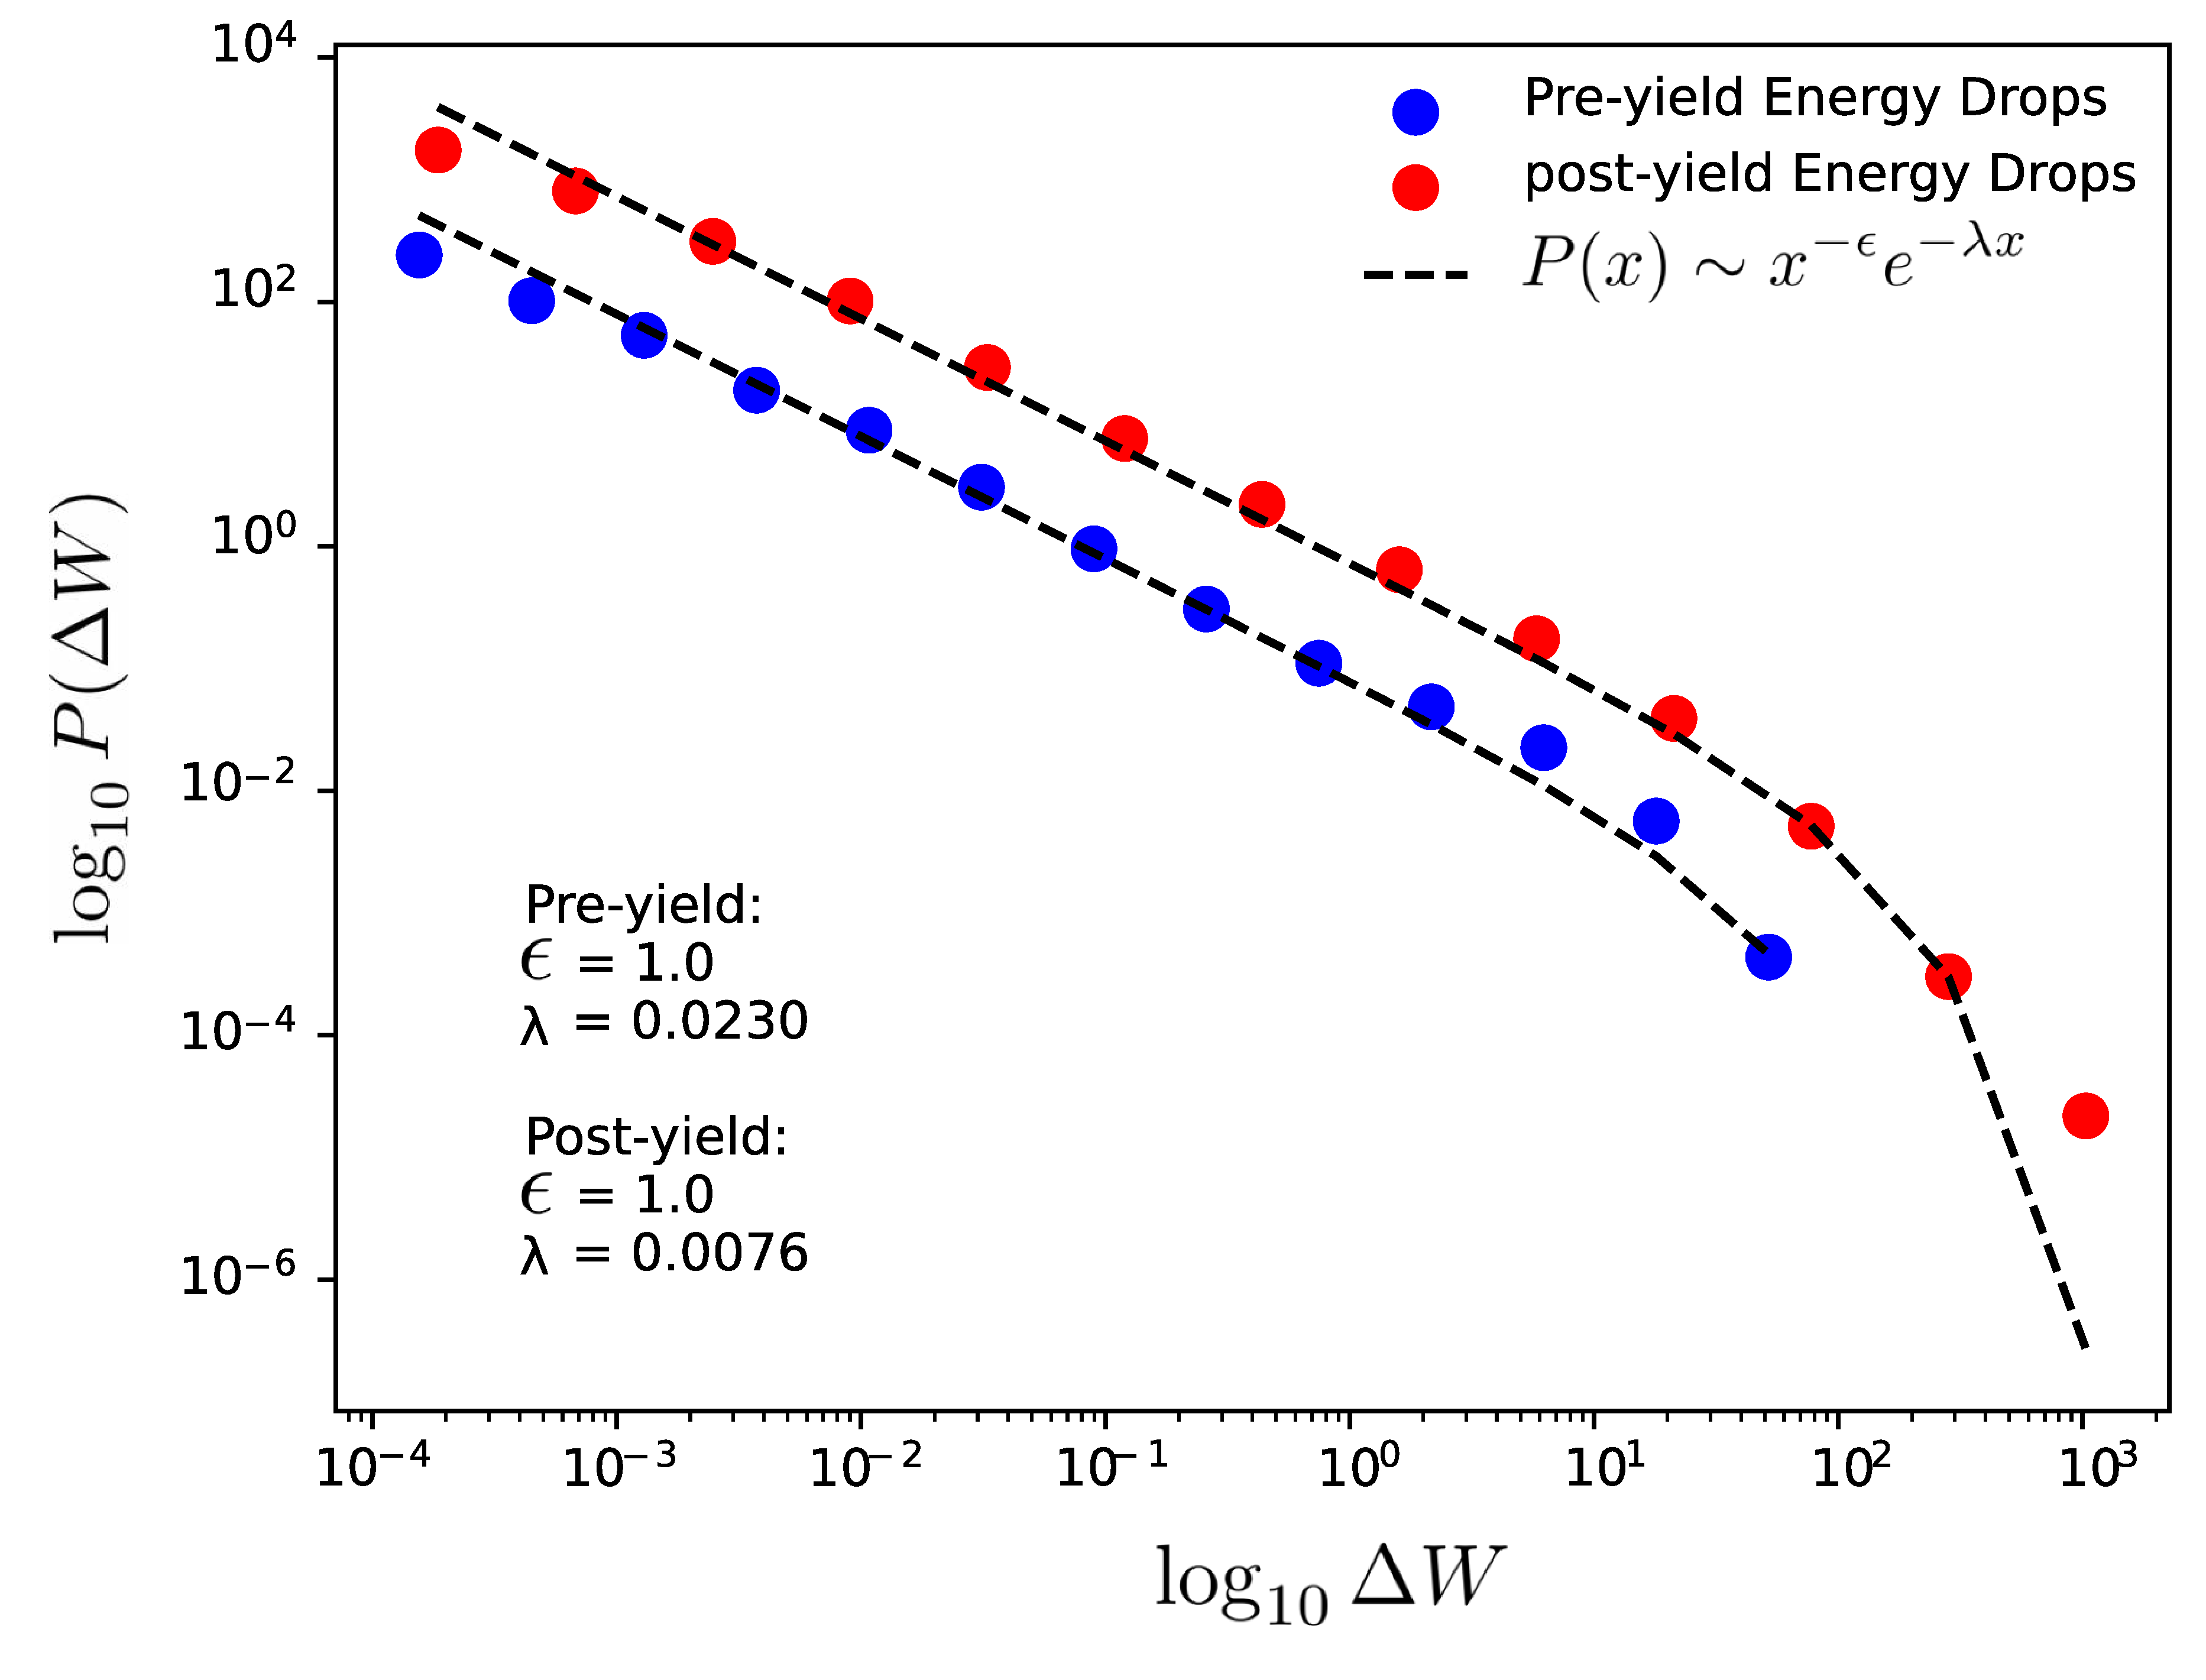
\includegraphics[scale=.1]{./Figures/Fig7.pdf}
\caption{Probability distribution of energy drops   during avalanches in pre- and post-yield  regimes. 
%Both distributions are well aprroximated by a power-law with exponential cutoff.  The power law exponents $\epsilon$ in both regimes are identical. Instead the  cutoff parameters  $\lambda$  are drastically different. 
}\label{fig:energy_drops}
\end{figure}


\begin{figure}[h!]
\centering
\begin{tabular}{cc}
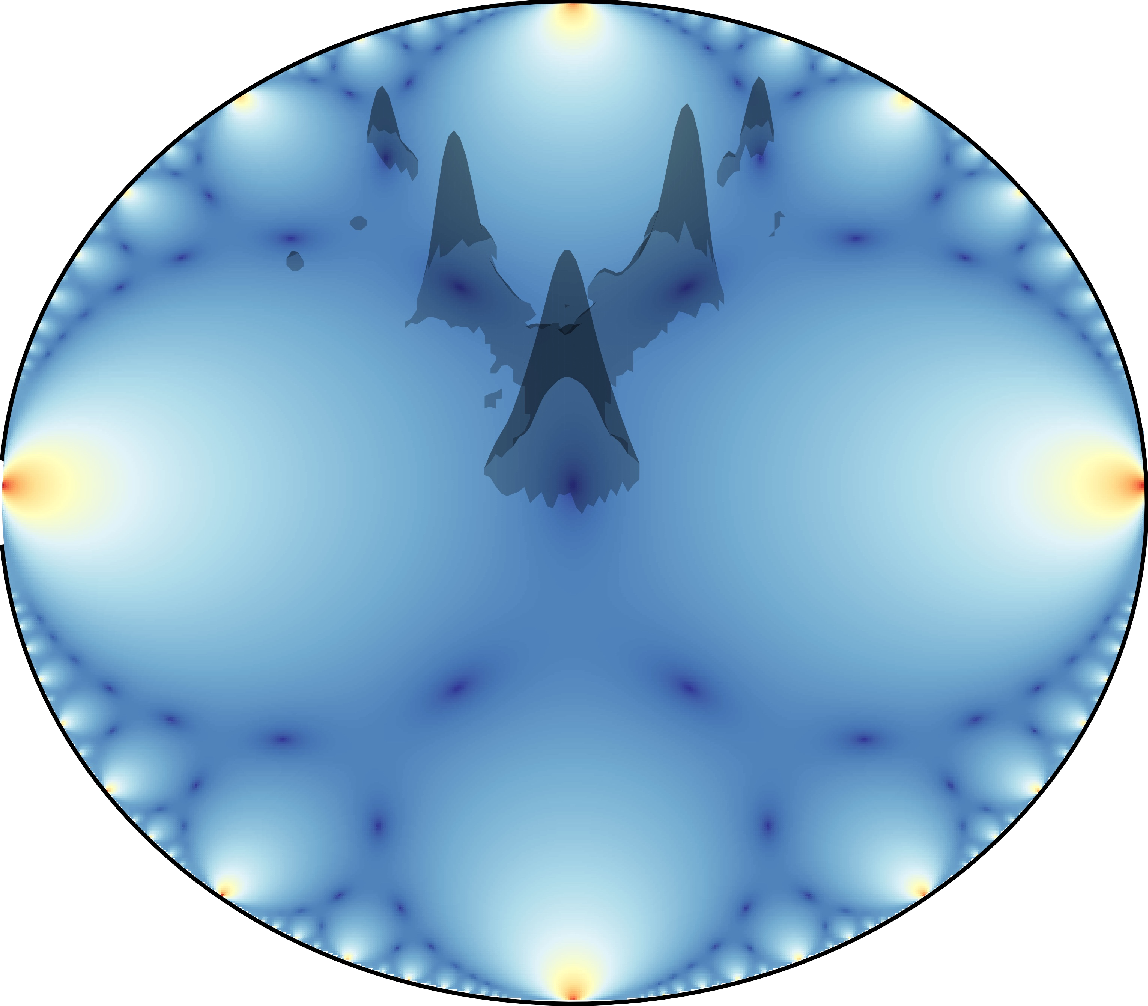
\includegraphics[scale=0.2]{./Figures/Fig8-a.pdf} &
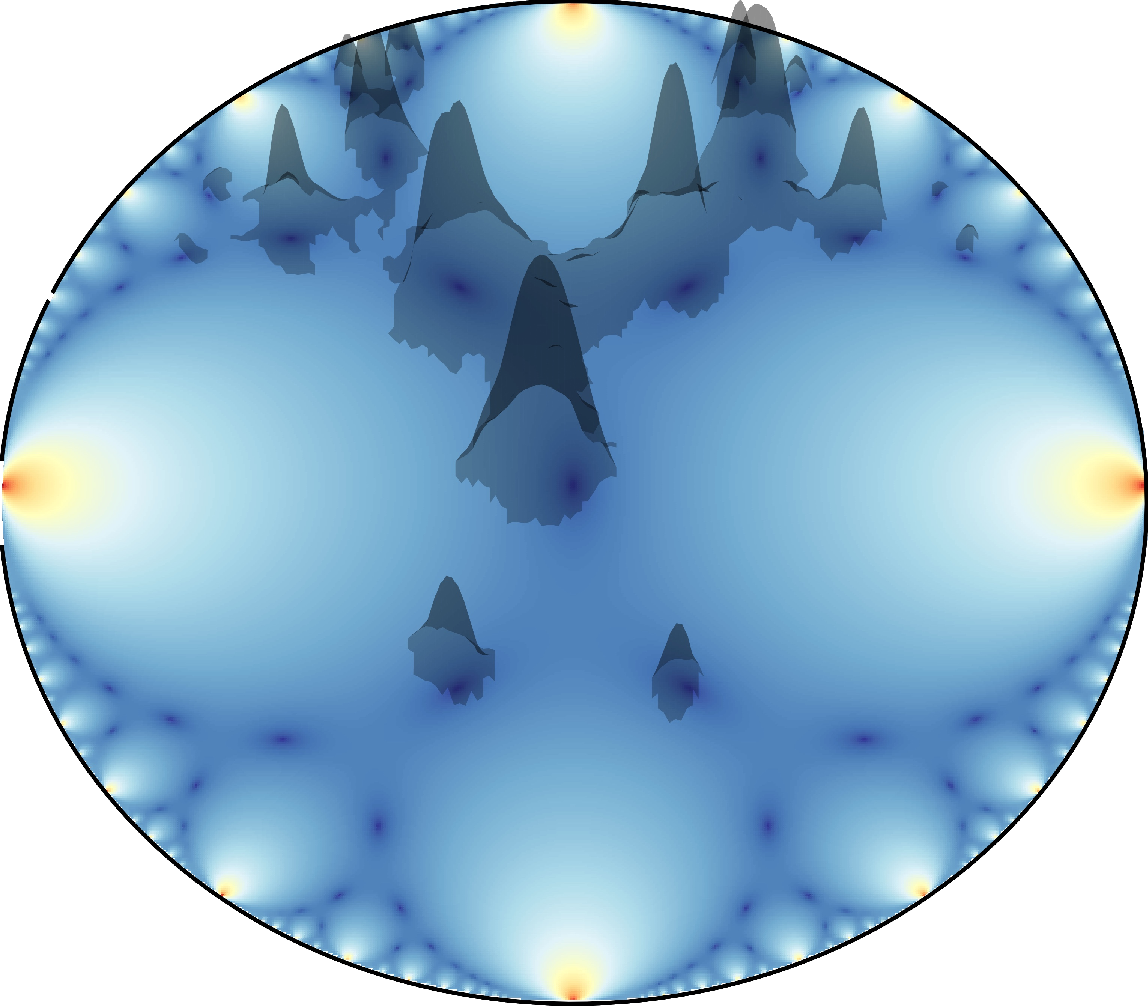
\includegraphics[scale=0.2]{./Figures/Fig8-b.pdf} \\
(a) Pre-yield ($\alpha \approx 0.3$) & (b) Post-yield ($\alpha \approx 0.8$) \\
\end{tabular}
\caption{Poincaré configurational space representations showing the height plot of occupied energy wells at different deformation stages. (a) In the pre-yield micro-plastic regime ($\alpha \approx 0.3$), mostly 3 wells are populated, showing the existence of dislocation gliding in the $x$ and $y$ directions. (b) In the post-yield regime ($\alpha \approx 0.8$), many more wells are populated due to the formation of shear bands and accumulated plastic deformation.}\label{fig:conf_space}
\end{figure}



The value of the power-law exponent $\epsilon = 1.0$ is a signature of an archetypically 'wild' crystal plasticity in the sense of \cite{Weiss2015-eh}. The same value was obtained in discrete dislocation dynamics studies of disorder-free 2D samples containing a fixed number of preexisting  dislocations \cite{Ispanovity2014-ra,PhysRevMaterials.5.073601} and was also recorded in numerical experiments on pristine crystals using a scalar version of the MTM \cite{Zhang2020-ax}. The exponent $\epsilon = 1.0$ has been previously interpreted in crystal plasticity framework as representing either dislocation jamming or self-induced glassiness \cite{Ovaska2015-yb,Lehtinen2016-qy,Zhang2016-gh}. 

It is rather striking that exactly the same value of the exponent has been also recorded in the studies of plastic flows in structural glasses~\cite{tyukodi2019avalanches,Ferrero2019-rx,Shang2020}. A theoretical understanding of the relation between the emergence of the power law exponent   $\epsilon=1.0$ and the structure of the underlying energy landscapes has been developed in the theory of spin glasses. Thus,  it was shown that the hierarchical (ultrametric) organization of energy wells in the phase space results in an intermittent, scale-free response to quasistatic deformation ~\cite{Franz2017-fa,Muller2015,Berthier2019-dm,Dennis2020-jb}. Moreover, it was rigorously proved   that in the mean-field limit the associated distribution of energy avalanches must be of a power law with exponent $\epsilon = 1.0$. In the spin glass context it has been also understood that the reason behind this particular value of the exponent is the marginal stability of the system ~\cite{Franz2017-fa,Pazmandi1999-lb,Le-Doussal2012-kv}.
 

Since glasses can be viewed as liquids at a quenching threshold, their marginal stability  is  similar to marginality  exhibited by  granular matter at a jamming point. If such  systems are mechanically driven, the proximity to unstable modes  leads to the mixing of statics (stability) and dynamics (instability) making the  mechanical response inherently  intermittent ~\cite{lamp2022brittle, rossi2022emergence}. Similarly, since  our 'quasi-amorphous crystal' emerged from arrested dynamics, one can argue that the associated  self-generated disorder   brought the system  from a solid to  an effectively  glassy state.  Furthermore, our results  suggest that the implied  marginality is  not   affected by the quasi-brittle yield,  which apparently does not compromise the global organization of the energy landscape while, of course,  affecting the reachability of its different subdomains~\cite{Regev2017-ks,Regev2017-jr,Regev2021-qf}.


%
% which implies that  the system was stabilized close to the associated threshold. 
%
%We can then argue that the outcome of  our 'proparation' protocol was 
%
% Since we observe the same 
%The fact that the value of the exponent $\epsilon = 1.0$ was observed in both pre- and post-yield regimes, 

Note next that the pre-yield  value of the cutoff parameter $\lambda = 0.0230$ is drastically different from its post-yield  value $\lambda = 0.0076$. The approximately three-fold decrease of the value of $\lambda$  indicates that large energy drops become substantially more probable in the post-yield regime ~\cite{Lin2014-bx,ruscher2021avalanches}. The emergent collective behavior  is reflected in  a much broader extent of avalanche activity which  reaches the size of the system  suggesting the divergence of the characteristic length $l \sim 1/\lambda$.   The physical nature of the implied  criticality  is presently actively  debated \cite{Grinstein1995-lw,Zippelius2023-ak,Charbonneau2023-oo,Oyama2023-oj,Xing2024-tz,Zhang2020-ax}.



%This conjecture is supported  by the observation  that  shear bands  in the post-yield regime   traverse the whole computational domain which is in   contrast to the  subextensive localized dislocation rearrangements  in the pre-yield regime.


%Finally we recall  that  intermittent fluctuations in amorphous plasticity are usually modeled in terms of 


Finally we mention that the observed similarity between the  structure of  intermittent plastic fluctuations in amorphous and crystalline solids is supported by the fact that elasto-plastic models, typically used to model amorphous plasticity  \cite{Nicolas2018-iy,PhysRevLett.129.228002,Ferrero2019-rx,Fernandez-Castellanos2021-yn}, are very similar to the MTM  which operates within basically the same finite element setting. The difference is that the phenomenological yield thresholds of elasto-plastic models are replaced in the MTM by elastic instabilities originating from the non-convexity of the  energy landscape. Accordingly,  the fixed linear elastic propagators are replaced by the solution 'on the fly' of the corresponding nonlinear elasticity problems. It is important   that the crucial   nonlinearity in the MTM is  of universal geometrical nature as it originates from the exact description of finite elastic deformations.

% 
%To conclude,  we used a novel mesoscopic tensorial model to achieve a deeper understanding of the phenomenon of plastic yield in crystals in the limit of zero strain rate and negligible thermal effects.

\textcolor{blue}{[Referee B: Finite Temperature] Temperature introduces a timescale causing "thermal rounding" of stress-strain peaks [Zhang et al., Acta Mater. 260, 119201 (2023); Li et al., arXiv:2409.16987 (2024)]. Our athermal limit represents the limit-envelope of these processes, where the universal scaling $\epsilon \approx 1.0$ is expected to persist despite mechanisms like climb becoming active at higher temperatures.}
 To conclude,  we  showed that mechanically driven perfect  crystals can exhibit   quasi-brittle plastic yielding which is remarkably similar  to the behavior  of well-annealed glassy materials. The implied parallel features of the mechanical response emerge after pristine crystals  acquire self-generated disorder  resulting  from  massive dislocation nucleation  during  the breakdown of an affine elastic configuration.  The ensuing quasi-amorphous crystals  exhibit  pre- and post-yield avalanches with  power law statistics whose  matching exponents are indicative of  the marginality  of the associated mechanical system.  Adaptation of the same  model to realistic 3D crystals will allow one to distinguish  between edge and screw dislocations opening the way to the adequate account  of such physically important  effects as dislocation climb, cross slip and forest hardening.
 
% It would  also be  also of interest to explore whether crystals with higher triangular symmetry exhibit similar behavior and to assess whether the specific choice of strain-energy density functional plays a crucial role in these phenomena. 

 %with HCP, FCC and BCC symmetry. In particular, only a 3D model will 
% 
 \emph{ Acknowledgments.} The authors thank N. Gorbushin,  S. Patinet, G. Tejedor   for helpful discussions. The work of O.U.S. was supported  by  the grants   ANR–21-CE08-MESOCRYSP, ANR-20-CE91-0010,  ANR-24-CE91-0002.   L. T.  was supported by the grants  ANR–21-CE08-MESOCRYSP and ERC-H2020-MSCA-RISE-2020-101008140.

%\bibliography{plasticity.bib}
%\bibliography{./formatted.bib}
%merlin.mbs apsrev4-1.bst 2010-07-25 4.21a (PWD, AO, DPC) hacked
%Control: key (0)
%Control: author (8) initials jnrlst
%Control: editor formatted (1) identically to author
%Control: production of article title (-1) disabled
%Control: page (0) single
%Control: year (1) truncated
%Control: production of eprint (0) enabled
\begin{thebibliography}{157}%
\makeatletter
\providecommand \@ifxundefined [1]{%
 \@ifx{#1\undefined}
}%
\providecommand \@ifnum [1]{%
 \ifnum #1\expandafter \@firstoftwo
 \else \expandafter \@secondoftwo
 \fi
}%
\providecommand \@ifx [1]{%
 \ifx #1\expandafter \@firstoftwo
 \else \expandafter \@secondoftwo
 \fi
}%
\providecommand \natexlab [1]{#1}%
\providecommand \enquote  [1]{``#1''}%
\providecommand \bibnamefont  [1]{#1}%
\providecommand \bibfnamefont [1]{#1}%
\providecommand \citenamefont [1]{#1}%
\providecommand \href@noop [0]{\@secondoftwo}%
\providecommand \href [0]{\begingroup \@sanitize@url \@href}%
\providecommand \@href[1]{\@@startlink{#1}\@@href}%
\providecommand \@@href[1]{\endgroup#1\@@endlink}%
\providecommand \@sanitize@url [0]{\catcode `\\12\catcode `\$12\catcode
  `\&12\catcode `\#12\catcode `\^12\catcode `\_12\catcode `\%12\relax}%
\providecommand \@@startlink[1]{}%
\providecommand \@@endlink[0]{}%
\providecommand \url  [0]{\begingroup\@sanitize@url \@url }%
\providecommand \@url [1]{\endgroup\@href {#1}{\urlprefix }}%
\providecommand \urlprefix  [0]{URL }%
\providecommand \Eprint [0]{\href }%
\providecommand \doibase [0]{http://dx.doi.org/}%
\providecommand \selectlanguage [0]{\@gobble}%
\providecommand \bibinfo  [0]{\@secondoftwo}%
\providecommand \bibfield  [0]{\@secondoftwo}%
\providecommand \translation [1]{[#1]}%
\providecommand \BibitemOpen [0]{}%
\providecommand \bibitemStop [0]{}%
\providecommand \bibitemNoStop [0]{.\EOS\space}%
\providecommand \EOS [0]{\spacefactor3000\relax}%
\providecommand \BibitemShut  [1]{\csname bibitem#1\endcsname}%
\let\auto@bib@innerbib\@empty
%</preamble>
\bibitem [{\citenamefont {Zaiser}(2006)}]{Zaiser2006-gk}%
  \BibitemOpen
  \bibfield  {author} {\bibinfo {author} {\bibfnamefont {M.}~\bibnamefont
  {Zaiser}},\ }\href@noop {} {\bibfield  {journal} {\bibinfo  {journal} {Adv.
  Phys.}\ }\textbf {\bibinfo {volume} {55}},\ \bibinfo {pages} {185} (\bibinfo
  {year} {2006})}\BibitemShut {NoStop}%
\bibitem [{\citenamefont {Jian}\ \emph {et~al.}(2024)\citenamefont {Jian},
  \citenamefont {Xiao}, \citenamefont {Sun},\ and\ \citenamefont
  {Cai}}]{jian2024prediction}%
  \BibitemOpen
  \bibfield  {author} {\bibinfo {author} {\bibfnamefont {W.}~\bibnamefont
  {Jian}}, \bibinfo {author} {\bibfnamefont {M.}~\bibnamefont {Xiao}}, \bibinfo
  {author} {\bibfnamefont {W.}~\bibnamefont {Sun}}, \ and\ \bibinfo {author}
  {\bibfnamefont {W.}~\bibnamefont {Cai}},\ }\href@noop {} {\bibfield
  {journal} {\bibinfo  {journal} {J. Mech. Phys. Solids}\ }\textbf {\bibinfo
  {volume} {186}},\ \bibinfo {pages} {105577} (\bibinfo {year}
  {2024})}\BibitemShut {NoStop}%
\bibitem [{\citenamefont {Ortiz}(1999)}]{ortiz1999plastic}%
  \BibitemOpen
  \bibfield  {author} {\bibinfo {author} {\bibfnamefont {M.}~\bibnamefont
  {Ortiz}},\ }\href@noop {} {\bibfield  {journal} {\bibinfo  {journal} {J.
  Appl. Mech.}\ }\textbf {\bibinfo {volume} {66}},\ \bibinfo {pages} {289}
  (\bibinfo {year} {1999})}\BibitemShut {NoStop}%
\bibitem [{\citenamefont {Papanikolaou}\ \emph {et~al.}(2017)\citenamefont
  {Papanikolaou}, \citenamefont {Cui},\ and\ \citenamefont
  {Ghoniem}}]{Papanikolaou2017-ld}%
  \BibitemOpen
  \bibfield  {author} {\bibinfo {author} {\bibfnamefont {S.}~\bibnamefont
  {Papanikolaou}}, \bibinfo {author} {\bibfnamefont {Y.}~\bibnamefont {Cui}}, \
  and\ \bibinfo {author} {\bibfnamefont {N.}~\bibnamefont {Ghoniem}},\
  }\href@noop {} {\bibfield  {journal} {\bibinfo  {journal} {Modell. Simul.
  Mater. Sci. Eng.}\ }\textbf {\bibinfo {volume} {26}},\ \bibinfo {pages}
  {013001} (\bibinfo {year} {2017})}\BibitemShut {NoStop}%
\bibitem [{\citenamefont {Kosterlitz}(2016)}]{kosterlitz2016kosterlitz}%
  \BibitemOpen
  \bibfield  {author} {\bibinfo {author} {\bibfnamefont {J.}~\bibnamefont
  {Kosterlitz}},\ }\href@noop {} {\bibfield  {journal} {\bibinfo  {journal}
  {Rep. Prog. Phys.}\ }\textbf {\bibinfo {volume} {79}},\ \bibinfo {pages}
  {026001} (\bibinfo {year} {2016})}\BibitemShut {NoStop}%
\bibitem [{\citenamefont {Khantha}\ and\ \citenamefont
  {Vitek}(1997)}]{khantha1997mechanism}%
  \BibitemOpen
  \bibfield  {author} {\bibinfo {author} {\bibfnamefont {M.}~\bibnamefont
  {Khantha}}\ and\ \bibinfo {author} {\bibfnamefont {V.}~\bibnamefont
  {Vitek}},\ }\href@noop {} {\bibfield  {journal} {\bibinfo  {journal} {Acta
  Mater.}\ }\textbf {\bibinfo {volume} {45}},\ \bibinfo {pages} {4675}
  (\bibinfo {year} {1997})}\BibitemShut {NoStop}%
\bibitem [{\citenamefont {Hochrainer}\ \emph {et~al.}(2014)\citenamefont
  {Hochrainer}, \citenamefont {Sandfeld}, \citenamefont {Zaiser},\ and\
  \citenamefont {Gumbsch}}]{hochrainer2014continuum}%
  \BibitemOpen
  \bibfield  {author} {\bibinfo {author} {\bibfnamefont {T.}~\bibnamefont
  {Hochrainer}}, \bibinfo {author} {\bibfnamefont {S.}~\bibnamefont
  {Sandfeld}}, \bibinfo {author} {\bibfnamefont {M.}~\bibnamefont {Zaiser}}, \
  and\ \bibinfo {author} {\bibfnamefont {P.}~\bibnamefont {Gumbsch}},\
  }\href@noop {} {\bibfield  {journal} {\bibinfo  {journal} {J. Mech. Phys.
  Solids}\ }\textbf {\bibinfo {volume} {63}},\ \bibinfo {pages} {167} (\bibinfo
  {year} {2014})}\BibitemShut {NoStop}%
\bibitem [{\citenamefont {Langer}(2019)}]{langer2019statistical}%
  \BibitemOpen
  \bibfield  {author} {\bibinfo {author} {\bibfnamefont {J.~S.}\ \bibnamefont
  {Langer}},\ }\href@noop {} {\bibfield  {journal} {\bibinfo  {journal} {J.
  Stat. Phys.}\ }\textbf {\bibinfo {volume} {175}},\ \bibinfo {pages} {531}
  (\bibinfo {year} {2019})}\BibitemShut {NoStop}%
\bibitem [{\citenamefont {Derlet}\ and\ \citenamefont
  {Maa{\ss}}(2016)}]{Derlet2016-mp}%
  \BibitemOpen
  \bibfield  {author} {\bibinfo {author} {\bibfnamefont {P.~M.}\ \bibnamefont
  {Derlet}}\ and\ \bibinfo {author} {\bibfnamefont {R.}~\bibnamefont
  {Maa{\ss}}},\ }\href@noop {} {\bibfield  {journal} {\bibinfo  {journal} {J.
  Appl. Phys.}\ }\textbf {\bibinfo {volume} {120}},\ \bibinfo {pages} {225101}
  (\bibinfo {year} {2016})}\BibitemShut {NoStop}%
\bibitem [{\citenamefont {Isp{\'a}novity}\ \emph {et~al.}(2010)\citenamefont
  {Isp{\'a}novity}, \citenamefont {Groma}, \citenamefont {Gy{\"o}rgyi},
  \citenamefont {Csikor},\ and\ \citenamefont
  {Weygand}}]{ispanovity2010submicron}%
  \BibitemOpen
  \bibfield  {author} {\bibinfo {author} {\bibfnamefont {P.~D.}\ \bibnamefont
  {Isp{\'a}novity}}, \bibinfo {author} {\bibfnamefont {I.}~\bibnamefont
  {Groma}}, \bibinfo {author} {\bibfnamefont {G.}~\bibnamefont {Gy{\"o}rgyi}},
  \bibinfo {author} {\bibfnamefont {F.~F.}\ \bibnamefont {Csikor}}, \ and\
  \bibinfo {author} {\bibfnamefont {D.}~\bibnamefont {Weygand}},\ }\href@noop
  {} {\bibfield  {journal} {\bibinfo  {journal} {Phys. Rev. Lett.}\ }\textbf
  {\bibinfo {volume} {105}},\ \bibinfo {pages} {085503} (\bibinfo {year}
  {2010})}\BibitemShut {NoStop}%
\bibitem [{\citenamefont {Kamani}\ and\ \citenamefont
  {Rogers}(2024)}]{kamani2024brittle}%
  \BibitemOpen
  \bibfield  {author} {\bibinfo {author} {\bibfnamefont {K.~M.}\ \bibnamefont
  {Kamani}}\ and\ \bibinfo {author} {\bibfnamefont {S.~A.}\ \bibnamefont
  {Rogers}},\ }\href@noop {} {\bibfield  {journal} {\bibinfo  {journal} {Proc.
  Natl. Acad. Sci. USA}\ }\textbf {\bibinfo {volume} {121}},\ \bibinfo {pages}
  {e2401409121} (\bibinfo {year} {2024})}\BibitemShut {NoStop}%
\bibitem [{\citenamefont {Berthier}\ \emph {et~al.}(2024)\citenamefont
  {Berthier}, \citenamefont {Biroli}, \citenamefont {Manning},\ and\
  \citenamefont {Zamponi}}]{berthier2024yielding}%
  \BibitemOpen
  \bibfield  {author} {\bibinfo {author} {\bibfnamefont {L.}~\bibnamefont
  {Berthier}}, \bibinfo {author} {\bibfnamefont {G.}~\bibnamefont {Biroli}},
  \bibinfo {author} {\bibfnamefont {M.~L.}\ \bibnamefont {Manning}}, \ and\
  \bibinfo {author} {\bibfnamefont {F.}~\bibnamefont {Zamponi}},\ }\href@noop
  {} {\bibfield  {journal} {\bibinfo  {journal} {arXiv preprint
  arXiv:2401.09385}\ } (\bibinfo {year} {2024})}\BibitemShut {NoStop}%
\bibitem [{\citenamefont {Shang}\ \emph {et~al.}(2020)\citenamefont {Shang},
  \citenamefont {Guan},\ and\ \citenamefont {Barrat}}]{Shang2020}%
  \BibitemOpen
  \bibfield  {author} {\bibinfo {author} {\bibfnamefont {B.}~\bibnamefont
  {Shang}}, \bibinfo {author} {\bibfnamefont {P.}~\bibnamefont {Guan}}, \ and\
  \bibinfo {author} {\bibfnamefont {J.~L.}\ \bibnamefont {Barrat}},\
  }\href@noop {} {\bibfield  {journal} {\bibinfo  {journal} {Proc. Natl. Acad.
  Sci.}\ }\textbf {\bibinfo {volume} {117}},\ \bibinfo {pages} {86} (\bibinfo
  {year} {2020})}\BibitemShut {NoStop}%
\bibitem [{\citenamefont {Shang}\ \emph {et~al.}(2024)\citenamefont {Shang},
  \citenamefont {Wang}, \citenamefont {Pan}, \citenamefont {Jin},\ and\
  \citenamefont {Zhang}}]{shang2024yielding}%
  \BibitemOpen
  \bibfield  {author} {\bibinfo {author} {\bibfnamefont {J.}~\bibnamefont
  {Shang}}, \bibinfo {author} {\bibfnamefont {Y.}~\bibnamefont {Wang}},
  \bibinfo {author} {\bibfnamefont {D.}~\bibnamefont {Pan}}, \bibinfo {author}
  {\bibfnamefont {Y.}~\bibnamefont {Jin}}, \ and\ \bibinfo {author}
  {\bibfnamefont {J.}~\bibnamefont {Zhang}},\ }\href@noop {} {\bibfield
  {journal} {\bibinfo  {journal} {Proc. Natl. Acad. Sci. USA}\ }\textbf
  {\bibinfo {volume} {121}},\ \bibinfo {pages} {e2402843121} (\bibinfo {year}
  {2024})}\BibitemShut {NoStop}%
\bibitem [{\citenamefont {Singh}\ \emph {et~al.}(2020)\citenamefont {Singh},
  \citenamefont {Ozawa},\ and\ \citenamefont {Berthier}}]{singh2020brittle}%
  \BibitemOpen
  \bibfield  {author} {\bibinfo {author} {\bibfnamefont {M.}~\bibnamefont
  {Singh}}, \bibinfo {author} {\bibfnamefont {M.}~\bibnamefont {Ozawa}}, \ and\
  \bibinfo {author} {\bibfnamefont {L.}~\bibnamefont {Berthier}},\ }\href@noop
  {} {\bibfield  {journal} {\bibinfo  {journal} {Phys. Rev. Mater.}\ }\textbf
  {\bibinfo {volume} {4}},\ \bibinfo {pages} {025603} (\bibinfo {year}
  {2020})}\BibitemShut {NoStop}%
\bibitem [{\citenamefont {Richard}\ \emph {et~al.}(2021)\citenamefont
  {Richard}, \citenamefont {Lerner},\ and\ \citenamefont
  {Bouchbinder}}]{richard2021brittle}%
  \BibitemOpen
  \bibfield  {author} {\bibinfo {author} {\bibfnamefont {D.}~\bibnamefont
  {Richard}}, \bibinfo {author} {\bibfnamefont {E.}~\bibnamefont {Lerner}}, \
  and\ \bibinfo {author} {\bibfnamefont {E.}~\bibnamefont {Bouchbinder}},\
  }\href@noop {} {\bibfield  {journal} {\bibinfo  {journal} {MRS Bull.}\
  }\textbf {\bibinfo {volume} {46}},\ \bibinfo {pages} {902} (\bibinfo {year}
  {2021})}\BibitemShut {NoStop}%
\bibitem [{\citenamefont {Pollard}\ and\ \citenamefont
  {Fielding}(2022)}]{pollard2022yielding}%
  \BibitemOpen
  \bibfield  {author} {\bibinfo {author} {\bibfnamefont {J.}~\bibnamefont
  {Pollard}}\ and\ \bibinfo {author} {\bibfnamefont {S.~M.}\ \bibnamefont
  {Fielding}},\ }\href@noop {} {\bibfield  {journal} {\bibinfo  {journal}
  {Phys. Rev. Res.}\ }\textbf {\bibinfo {volume} {4}},\ \bibinfo {pages}
  {043037} (\bibinfo {year} {2022})}\BibitemShut {NoStop}%
\bibitem [{\citenamefont {Lin}\ \emph {et~al.}(2014)\citenamefont {Lin},
  \citenamefont {Lerner}, \citenamefont {Rosso},\ and\ \citenamefont
  {Wyart}}]{Lin2014-bx}%
  \BibitemOpen
  \bibfield  {author} {\bibinfo {author} {\bibfnamefont {J.}~\bibnamefont
  {Lin}}, \bibinfo {author} {\bibfnamefont {E.}~\bibnamefont {Lerner}},
  \bibinfo {author} {\bibfnamefont {A.}~\bibnamefont {Rosso}}, \ and\ \bibinfo
  {author} {\bibfnamefont {M.}~\bibnamefont {Wyart}},\ }\href@noop {}
  {\bibfield  {journal} {\bibinfo  {journal} {Proc. Natl. Acad. Sci. U. S. A.}\
  }\textbf {\bibinfo {volume} {111}},\ \bibinfo {pages} {14382} (\bibinfo
  {year} {2014})}\BibitemShut {NoStop}%
\bibitem [{\citenamefont {Parisi}\ \emph {et~al.}(2017)\citenamefont {Parisi},
  \citenamefont {Procaccia}, \citenamefont {Rainone},\ and\ \citenamefont
  {Singh}}]{parisi2017shear}%
  \BibitemOpen
  \bibfield  {author} {\bibinfo {author} {\bibfnamefont {G.}~\bibnamefont
  {Parisi}}, \bibinfo {author} {\bibfnamefont {I.}~\bibnamefont {Procaccia}},
  \bibinfo {author} {\bibfnamefont {C.}~\bibnamefont {Rainone}}, \ and\
  \bibinfo {author} {\bibfnamefont {M.}~\bibnamefont {Singh}},\ }\href@noop {}
  {\bibfield  {journal} {\bibinfo  {journal} {Proc. Natl. Acad. Sci. USA}\
  }\textbf {\bibinfo {volume} {114}},\ \bibinfo {pages} {5577} (\bibinfo {year}
  {2017})}\BibitemShut {NoStop}%
\bibitem [{\citenamefont {Derlet}\ and\ \citenamefont
  {Maa{\ss}}(2021)}]{derlet2021micro}%
  \BibitemOpen
  \bibfield  {author} {\bibinfo {author} {\bibfnamefont {P.~M.}\ \bibnamefont
  {Derlet}}\ and\ \bibinfo {author} {\bibfnamefont {R.}~\bibnamefont
  {Maa{\ss}}},\ }\href@noop {} {\bibfield  {journal} {\bibinfo  {journal} {Acta
  Mater.}\ }\textbf {\bibinfo {volume} {209}},\ \bibinfo {pages} {116771}
  (\bibinfo {year} {2021})}\BibitemShut {NoStop}%
\bibitem [{\citenamefont {Lehtinen}\ \emph {et~al.}(2016)\citenamefont
  {Lehtinen}, \citenamefont {Costantini}, \citenamefont {Alava}, \citenamefont
  {Zapperi},\ and\ \citenamefont {Laurson}}]{Lehtinen2016-qy}%
  \BibitemOpen
  \bibfield  {author} {\bibinfo {author} {\bibfnamefont {A.}~\bibnamefont
  {Lehtinen}}, \bibinfo {author} {\bibfnamefont {G.}~\bibnamefont
  {Costantini}}, \bibinfo {author} {\bibfnamefont {M.~J.}\ \bibnamefont
  {Alava}}, \bibinfo {author} {\bibfnamefont {S.}~\bibnamefont {Zapperi}}, \
  and\ \bibinfo {author} {\bibfnamefont {L.}~\bibnamefont {Laurson}},\
  }\href@noop {} {\bibfield  {journal} {\bibinfo  {journal} {Phys. Rev. B}\
  }\textbf {\bibinfo {volume} {94}},\ \bibinfo {pages} {064101} (\bibinfo
  {year} {2016})}\BibitemShut {NoStop}%
\bibitem [{\citenamefont {Sethna}\ \emph {et~al.}(2017)\citenamefont {Sethna},
  \citenamefont {Bierbaum}, \citenamefont {Dahmen}, \citenamefont {Goodrich},
  \citenamefont {Greer}, \citenamefont {Hayden},\ and\ \citenamefont
  {Zapperi}}]{Sethna2017}%
  \BibitemOpen
  \bibfield  {author} {\bibinfo {author} {\bibfnamefont {J.~P.}\ \bibnamefont
  {Sethna}}, \bibinfo {author} {\bibfnamefont {M.~K.}\ \bibnamefont
  {Bierbaum}}, \bibinfo {author} {\bibfnamefont {K.~A.}\ \bibnamefont
  {Dahmen}}, \bibinfo {author} {\bibfnamefont {C.~P.}\ \bibnamefont
  {Goodrich}}, \bibinfo {author} {\bibfnamefont {J.~R.}\ \bibnamefont {Greer}},
  \bibinfo {author} {\bibfnamefont {L.~X.}\ \bibnamefont {Hayden}}, \ and\
  \bibinfo {author} {\bibfnamefont {S.}~\bibnamefont {Zapperi}},\ }\href@noop
  {} {\bibfield  {journal} {\bibinfo  {journal} {Annu. Rev. Mater. Res.}\
  }\textbf {\bibinfo {volume} {47}},\ \bibinfo {pages} {217} (\bibinfo {year}
  {2017})}\BibitemShut {NoStop}%
\bibitem [{\citenamefont {Ovaska}\ \emph {et~al.}(2017)\citenamefont {Ovaska},
  \citenamefont {Lehtinen}, \citenamefont {Alava}, \citenamefont {Laurson},\
  and\ \citenamefont {Zapperi}}]{Ovaska2017}%
  \BibitemOpen
  \bibfield  {author} {\bibinfo {author} {\bibfnamefont {M.}~\bibnamefont
  {Ovaska}}, \bibinfo {author} {\bibfnamefont {A.}~\bibnamefont {Lehtinen}},
  \bibinfo {author} {\bibfnamefont {M.~J.}\ \bibnamefont {Alava}}, \bibinfo
  {author} {\bibfnamefont {L.}~\bibnamefont {Laurson}}, \ and\ \bibinfo
  {author} {\bibfnamefont {S.}~\bibnamefont {Zapperi}},\ }\href@noop {}
  {\bibfield  {journal} {\bibinfo  {journal} {Phys. Rev. Lett.}\ }\textbf
  {\bibinfo {volume} {119}},\ \bibinfo {pages} {265501} (\bibinfo {year}
  {2017})}\BibitemShut {NoStop}%
\bibitem [{\citenamefont {Nicolas}\ \emph {et~al.}(2018)\citenamefont
  {Nicolas}, \citenamefont {Ferrero}, \citenamefont {Martens},\ and\
  \citenamefont {Barrat}}]{Nicolas2018-iy}%
  \BibitemOpen
  \bibfield  {author} {\bibinfo {author} {\bibfnamefont {A.}~\bibnamefont
  {Nicolas}}, \bibinfo {author} {\bibfnamefont {E.~E.}\ \bibnamefont
  {Ferrero}}, \bibinfo {author} {\bibfnamefont {K.}~\bibnamefont {Martens}}, \
  and\ \bibinfo {author} {\bibfnamefont {J.}~\bibnamefont {Barrat}},\
  }\href@noop {} {\bibfield  {journal} {\bibinfo  {journal} {Rev. Mod. Phys.}\
  }\textbf {\bibinfo {volume} {90}} (\bibinfo {year} {2018})}\BibitemShut
  {NoStop}%
\bibitem [{\citenamefont {Rodney}\ \emph {et~al.}(2011)\citenamefont {Rodney},
  \citenamefont {Tanguy},\ and\ \citenamefont {Vandembroucq}}]{Rodney2011-ld}%
  \BibitemOpen
  \bibfield  {author} {\bibinfo {author} {\bibfnamefont {D.}~\bibnamefont
  {Rodney}}, \bibinfo {author} {\bibfnamefont {A.}~\bibnamefont {Tanguy}}, \
  and\ \bibinfo {author} {\bibfnamefont {D.}~\bibnamefont {Vandembroucq}},\
  }\href@noop {} {\bibfield  {journal} {\bibinfo  {journal} {Model. Simul. Mat.
  Sci. Eng.}\ }\textbf {\bibinfo {volume} {19}},\ \bibinfo {pages} {083001}
  (\bibinfo {year} {2011})}\BibitemShut {NoStop}%
\bibitem [{\citenamefont {Popovi{\'c}}\ \emph {et~al.}(2018)\citenamefont
  {Popovi{\'c}}, \citenamefont {de~Geus},\ and\ \citenamefont
  {Wyart}}]{popovic2018elastoplastic}%
  \BibitemOpen
  \bibfield  {author} {\bibinfo {author} {\bibfnamefont {M.}~\bibnamefont
  {Popovi{\'c}}}, \bibinfo {author} {\bibfnamefont {T.~W.~J.}\ \bibnamefont
  {de~Geus}}, \ and\ \bibinfo {author} {\bibfnamefont {M.}~\bibnamefont
  {Wyart}},\ }\href@noop {} {\bibfield  {journal} {\bibinfo  {journal} {Phys.
  Rev. E}\ }\textbf {\bibinfo {volume} {98}},\ \bibinfo {pages} {040901}
  (\bibinfo {year} {2018})}\BibitemShut {NoStop}%
\bibitem [{\citenamefont {Tanguy}(2021)}]{Tanguy2021-ap}%
  \BibitemOpen
  \bibfield  {author} {\bibinfo {author} {\bibfnamefont {A.}~\bibnamefont
  {Tanguy}},\ }\href@noop {} {\bibfield  {journal} {\bibinfo  {journal} {C. R.
  Phys.}\ }\textbf {\bibinfo {volume} {22}},\ \bibinfo {pages} {117} (\bibinfo
  {year} {2021})}\BibitemShut {NoStop}%
\bibitem [{\citenamefont {Talamali}\ \emph {et~al.}(2012)\citenamefont
  {Talamali}, \citenamefont {Pet{\"a}j{\"a}}, \citenamefont {Vandembroucq},\
  and\ \citenamefont {Roux}}]{TALAMALI2012275}%
  \BibitemOpen
  \bibfield  {author} {\bibinfo {author} {\bibfnamefont {M.}~\bibnamefont
  {Talamali}}, \bibinfo {author} {\bibfnamefont {V.}~\bibnamefont
  {Pet{\"a}j{\"a}}}, \bibinfo {author} {\bibfnamefont {D.}~\bibnamefont
  {Vandembroucq}}, \ and\ \bibinfo {author} {\bibfnamefont {S.}~\bibnamefont
  {Roux}},\ }\href@noop {} {\bibfield  {journal} {\bibinfo  {journal} {C. R.
  M{\'e}canique}\ }\textbf {\bibinfo {volume} {340}},\ \bibinfo {pages} {275}
  (\bibinfo {year} {2012})}\BibitemShut {NoStop}%
\bibitem [{\citenamefont {Parley}\ and\ \citenamefont
  {Sollich}(2024)}]{Parley2024-jb}%
  \BibitemOpen
  \bibfield  {author} {\bibinfo {author} {\bibfnamefont {J.~T.}\ \bibnamefont
  {Parley}}\ and\ \bibinfo {author} {\bibfnamefont {P.}~\bibnamefont
  {Sollich}},\ }\href@noop {} {\bibfield  {journal} {\bibinfo  {journal} {Phys.
  Rev. E.}\ }\textbf {\bibinfo {volume} {110}},\ \bibinfo {pages} {045002}
  (\bibinfo {year} {2024})}\BibitemShut {NoStop}%
\bibitem [{\citenamefont {Karmakar}\ \emph {et~al.}(2010)\citenamefont
  {Karmakar}, \citenamefont {Lerner},\ and\ \citenamefont
  {Procaccia}}]{karmakar2010statistical}%
  \BibitemOpen
  \bibfield  {author} {\bibinfo {author} {\bibfnamefont {S.}~\bibnamefont
  {Karmakar}}, \bibinfo {author} {\bibfnamefont {E.}~\bibnamefont {Lerner}}, \
  and\ \bibinfo {author} {\bibfnamefont {I.}~\bibnamefont {Procaccia}},\
  }\href@noop {} {\bibfield  {journal} {\bibinfo  {journal} {Phys. Rev. E Stat.
  Nonlin. Soft Matter Phys.}\ }\textbf {\bibinfo {volume} {82}},\ \bibinfo
  {pages} {055103} (\bibinfo {year} {2010})}\BibitemShut {NoStop}%
\bibitem [{\citenamefont {Ozawa}\ \emph {et~al.}(2018)\citenamefont {Ozawa},
  \citenamefont {Berthier}, \citenamefont {Biroli}, \citenamefont {Rosso},\
  and\ \citenamefont {Tarjus}}]{ozawa2018random}%
  \BibitemOpen
  \bibfield  {author} {\bibinfo {author} {\bibfnamefont {M.}~\bibnamefont
  {Ozawa}}, \bibinfo {author} {\bibfnamefont {L.}~\bibnamefont {Berthier}},
  \bibinfo {author} {\bibfnamefont {G.}~\bibnamefont {Biroli}}, \bibinfo
  {author} {\bibfnamefont {A.}~\bibnamefont {Rosso}}, \ and\ \bibinfo {author}
  {\bibfnamefont {G.}~\bibnamefont {Tarjus}},\ }\href@noop {} {\bibfield
  {journal} {\bibinfo  {journal} {Proc. Natl. Acad. Sci.}\ }\textbf {\bibinfo
  {volume} {115}},\ \bibinfo {pages} {6656} (\bibinfo {year}
  {2018})}\BibitemShut {NoStop}%
\bibitem [{\citenamefont {Divoux}\ \emph {et~al.}(2024)\citenamefont {Divoux},
  \citenamefont {Agoritsas}, \citenamefont {Aime}, \citenamefont {Barentin},
  \citenamefont {Barrat}, \citenamefont {Benzi}, \citenamefont {Berthier},
  \citenamefont {Bi}, \citenamefont {Biroli}, \citenamefont {Bonn},
  \citenamefont {Bourrianne}, \citenamefont {Bouzid}, \citenamefont {Del~Gado},
  \citenamefont {Delanoe-Ayari}, \citenamefont {Farain}, \citenamefont
  {Fielding}, \citenamefont {Fuchs}, \citenamefont {van~der Gucht},
  \citenamefont {Henkes}, \citenamefont {Jalaal}, \citenamefont {Joshi},
  \citenamefont {Lemaitre}, \citenamefont {Leheny}, \citenamefont {Manneville},
  \citenamefont {Martens}, \citenamefont {Poon}, \citenamefont {Popovic},
  \citenamefont {Procaccia}, \citenamefont {Ramos}, \citenamefont {Richards},
  \citenamefont {Rogers}, \citenamefont {Rossi}, \citenamefont {Sbragaglia},
  \citenamefont {Tarjus}, \citenamefont {Toschi}, \citenamefont {Trappe},
  \citenamefont {Vermant}, \citenamefont {Wyart}, \citenamefont {Zamponi},\
  and\ \citenamefont {Zare}}]{Divoux2024-ks}%
  \BibitemOpen
  \bibfield  {author} {\bibinfo {author} {\bibfnamefont {T.}~\bibnamefont
  {Divoux}}, \bibinfo {author} {\bibfnamefont {E.}~\bibnamefont {Agoritsas}},
  \bibinfo {author} {\bibfnamefont {S.}~\bibnamefont {Aime}}, \bibinfo {author}
  {\bibfnamefont {C.}~\bibnamefont {Barentin}}, \bibinfo {author}
  {\bibfnamefont {J.-L.}\ \bibnamefont {Barrat}}, \bibinfo {author}
  {\bibfnamefont {R.}~\bibnamefont {Benzi}}, \bibinfo {author} {\bibfnamefont
  {L.}~\bibnamefont {Berthier}}, \bibinfo {author} {\bibfnamefont
  {D.}~\bibnamefont {Bi}}, \bibinfo {author} {\bibfnamefont {G.}~\bibnamefont
  {Biroli}}, \bibinfo {author} {\bibfnamefont {D.}~\bibnamefont {Bonn}},
  \bibinfo {author} {\bibfnamefont {P.}~\bibnamefont {Bourrianne}}, \bibinfo
  {author} {\bibfnamefont {M.}~\bibnamefont {Bouzid}}, \bibinfo {author}
  {\bibfnamefont {E.}~\bibnamefont {Del~Gado}}, \bibinfo {author}
  {\bibfnamefont {H.}~\bibnamefont {Delanoe-Ayari}}, \bibinfo {author}
  {\bibfnamefont {K.}~\bibnamefont {Farain}}, \bibinfo {author} {\bibfnamefont
  {S.}~\bibnamefont {Fielding}}, \bibinfo {author} {\bibfnamefont
  {M.}~\bibnamefont {Fuchs}}, \bibinfo {author} {\bibfnamefont
  {J.}~\bibnamefont {van~der Gucht}}, \bibinfo {author} {\bibfnamefont
  {S.}~\bibnamefont {Henkes}}, \bibinfo {author} {\bibfnamefont
  {M.}~\bibnamefont {Jalaal}}, \bibinfo {author} {\bibfnamefont {Y.~M.}\
  \bibnamefont {Joshi}}, \bibinfo {author} {\bibfnamefont {A.}~\bibnamefont
  {Lemaitre}}, \bibinfo {author} {\bibfnamefont {R.~L.}\ \bibnamefont
  {Leheny}}, \bibinfo {author} {\bibfnamefont {S.}~\bibnamefont {Manneville}},
  \bibinfo {author} {\bibfnamefont {K.}~\bibnamefont {Martens}}, \bibinfo
  {author} {\bibfnamefont {W.~C.~K.}\ \bibnamefont {Poon}}, \bibinfo {author}
  {\bibfnamefont {M.}~\bibnamefont {Popovic}}, \bibinfo {author} {\bibfnamefont
  {I.}~\bibnamefont {Procaccia}}, \bibinfo {author} {\bibfnamefont
  {L.}~\bibnamefont {Ramos}}, \bibinfo {author} {\bibfnamefont {J.~A.}\
  \bibnamefont {Richards}}, \bibinfo {author} {\bibfnamefont {S.}~\bibnamefont
  {Rogers}}, \bibinfo {author} {\bibfnamefont {S.}~\bibnamefont {Rossi}},
  \bibinfo {author} {\bibfnamefont {M.}~\bibnamefont {Sbragaglia}}, \bibinfo
  {author} {\bibfnamefont {G.}~\bibnamefont {Tarjus}}, \bibinfo {author}
  {\bibfnamefont {F.}~\bibnamefont {Toschi}}, \bibinfo {author} {\bibfnamefont
  {V.}~\bibnamefont {Trappe}}, \bibinfo {author} {\bibfnamefont
  {J.}~\bibnamefont {Vermant}}, \bibinfo {author} {\bibfnamefont
  {M.}~\bibnamefont {Wyart}}, \bibinfo {author} {\bibfnamefont
  {F.}~\bibnamefont {Zamponi}}, \ and\ \bibinfo {author} {\bibfnamefont
  {D.}~\bibnamefont {Zare}},\ }\href@noop {} {\bibfield  {journal} {\bibinfo
  {journal} {Soft Matter}\ }\textbf {\bibinfo {volume} {20}},\ \bibinfo {pages}
  {6868} (\bibinfo {year} {2024})}\BibitemShut {NoStop}%
\bibitem [{\citenamefont {Moshe}\ \emph {et~al.}(2015)\citenamefont {Moshe},
  \citenamefont {Levin}, \citenamefont {Aharoni}, \citenamefont {Kupferman},\
  and\ \citenamefont {Sharon}}]{Moshe2015-rm}%
  \BibitemOpen
  \bibfield  {author} {\bibinfo {author} {\bibfnamefont {M.}~\bibnamefont
  {Moshe}}, \bibinfo {author} {\bibfnamefont {I.}~\bibnamefont {Levin}},
  \bibinfo {author} {\bibfnamefont {H.}~\bibnamefont {Aharoni}}, \bibinfo
  {author} {\bibfnamefont {R.}~\bibnamefont {Kupferman}}, \ and\ \bibinfo
  {author} {\bibfnamefont {E.}~\bibnamefont {Sharon}},\ }\href@noop {}
  {\bibfield  {journal} {\bibinfo  {journal} {Proc. Natl. Acad. Sci.}\ }\textbf
  {\bibinfo {volume} {112}},\ \bibinfo {pages} {10873} (\bibinfo {year}
  {2015})}\BibitemShut {NoStop}%
\bibitem [{\citenamefont {Baggioli}\ \emph {et~al.}(2022)\citenamefont
  {Baggioli}, \citenamefont {Landry},\ and\ \citenamefont
  {Zaccone}}]{Baggioli2022-nx}%
  \BibitemOpen
  \bibfield  {author} {\bibinfo {author} {\bibfnamefont {M.}~\bibnamefont
  {Baggioli}}, \bibinfo {author} {\bibfnamefont {M.}~\bibnamefont {Landry}}, \
  and\ \bibinfo {author} {\bibfnamefont {A.}~\bibnamefont {Zaccone}},\
  }\href@noop {} {\bibfield  {journal} {\bibinfo  {journal} {Phys. Rev. E.}\
  }\textbf {\bibinfo {volume} {105}},\ \bibinfo {pages} {024602} (\bibinfo
  {year} {2022})}\BibitemShut {NoStop}%
\bibitem [{\citenamefont {Bowick}\ and\ \citenamefont
  {Giomi}(2009)}]{Bowick2009-bl}%
  \BibitemOpen
  \bibfield  {author} {\bibinfo {author} {\bibfnamefont {M.~J.}\ \bibnamefont
  {Bowick}}\ and\ \bibinfo {author} {\bibfnamefont {L.}~\bibnamefont {Giomi}},\
  }\href@noop {} {\bibfield  {journal} {\bibinfo  {journal} {Adv. Phys.}\
  }\textbf {\bibinfo {volume} {58}},\ \bibinfo {pages} {449} (\bibinfo {year}
  {2009})}\BibitemShut {NoStop}%
\bibitem [{\citenamefont {Katanaev}\ and\ \citenamefont
  {Volovich}(1992)}]{Katanaev1992-kl}%
  \BibitemOpen
  \bibfield  {author} {\bibinfo {author} {\bibfnamefont {M.}~\bibnamefont
  {Katanaev}}\ and\ \bibinfo {author} {\bibfnamefont {I.}~\bibnamefont
  {Volovich}},\ }\href@noop {} {\bibfield  {journal} {\bibinfo  {journal}
  {Annals of Physics}\ }\textbf {\bibinfo {volume} {216}},\ \bibinfo {pages}
  {1} (\bibinfo {year} {1992})}\BibitemShut {NoStop}%
\bibitem [{\citenamefont {Sozio}\ and\ \citenamefont
  {Yavari}(2020)}]{Sozio2020-tg}%
  \BibitemOpen
  \bibfield  {author} {\bibinfo {author} {\bibfnamefont {F.}~\bibnamefont
  {Sozio}}\ and\ \bibinfo {author} {\bibfnamefont {A.}~\bibnamefont {Yavari}},\
  }\href@noop {} {\bibfield  {journal} {\bibinfo  {journal} {Math. Mech.
  Solids}\ }\textbf {\bibinfo {volume} {25}},\ \bibinfo {pages} {1267}
  (\bibinfo {year} {2020})}\BibitemShut {NoStop}%
\bibitem [{\citenamefont {Picard}\ \emph {et~al.}(2004)\citenamefont {Picard},
  \citenamefont {Ajdari}, \citenamefont {Lequeux},\ and\ \citenamefont
  {Bocquet}}]{Picard2004}%
  \BibitemOpen
  \bibfield  {author} {\bibinfo {author} {\bibfnamefont {G.}~\bibnamefont
  {Picard}}, \bibinfo {author} {\bibfnamefont {A.}~\bibnamefont {Ajdari}},
  \bibinfo {author} {\bibfnamefont {F.}~\bibnamefont {Lequeux}}, \ and\
  \bibinfo {author} {\bibfnamefont {L.}~\bibnamefont {Bocquet}},\ }\href@noop
  {} {\bibfield  {journal} {\bibinfo  {journal} {Europhysics Journal E}\
  }\textbf {\bibinfo {volume} {15}},\ \bibinfo {pages} {371} (\bibinfo {year}
  {2004})}\BibitemShut {NoStop}%
\bibitem [{\citenamefont {Budrikis}\ \emph {et~al.}(2017)\citenamefont
  {Budrikis}, \citenamefont {Castellanos}, \citenamefont {Sandfeld},
  \citenamefont {Zaiser},\ and\ \citenamefont {Zapperi}}]{Budrikis2017-ex}%
  \BibitemOpen
  \bibfield  {author} {\bibinfo {author} {\bibfnamefont {Z.}~\bibnamefont
  {Budrikis}}, \bibinfo {author} {\bibfnamefont {D.}~\bibnamefont
  {Castellanos}}, \bibinfo {author} {\bibfnamefont {S.}~\bibnamefont
  {Sandfeld}}, \bibinfo {author} {\bibfnamefont {M.}~\bibnamefont {Zaiser}}, \
  and\ \bibinfo {author} {\bibfnamefont {S.}~\bibnamefont {Zapperi}},\
  }\href@noop {} {\bibfield  {journal} {\bibinfo  {journal} {Nat. Commun.}\
  }\textbf {\bibinfo {volume} {8}},\ \bibinfo {pages} {15928} (\bibinfo {year}
  {2017})}\BibitemShut {NoStop}%
\bibitem [{\citenamefont {Cai}\ \emph {et~al.}(2006)\citenamefont {Cai},
  \citenamefont {Arsenlis}, \citenamefont {Weinberger},\ and\ \citenamefont
  {Bulatov}}]{Cai2006-fe}%
  \BibitemOpen
  \bibfield  {author} {\bibinfo {author} {\bibfnamefont {W.}~\bibnamefont
  {Cai}}, \bibinfo {author} {\bibfnamefont {A.}~\bibnamefont {Arsenlis}},
  \bibinfo {author} {\bibfnamefont {C.~R.}\ \bibnamefont {Weinberger}}, \ and\
  \bibinfo {author} {\bibfnamefont {V.~V.}\ \bibnamefont {Bulatov}},\
  }\href@noop {} {\bibfield  {journal} {\bibinfo  {journal} {J. Mech. Phys.
  Solids}\ }\textbf {\bibinfo {volume} {54}},\ \bibinfo {pages} {561} (\bibinfo
  {year} {2006})}\BibitemShut {NoStop}%
\bibitem [{\citenamefont {Salman}\ and\ \citenamefont
  {Truskinovsky}(2011)}]{Salman2011}%
  \BibitemOpen
  \bibfield  {author} {\bibinfo {author} {\bibfnamefont {O.~U.}\ \bibnamefont
  {Salman}}\ and\ \bibinfo {author} {\bibfnamefont {L.}~\bibnamefont
  {Truskinovsky}},\ }\href@noop {} {\bibfield  {journal} {\bibinfo  {journal}
  {Phys. Rev. Lett.}\ }\textbf {\bibinfo {volume} {106}},\ \bibinfo {pages}
  {175503} (\bibinfo {year} {2011})}\BibitemShut {NoStop}%
\bibitem [{\citenamefont {Salman}\ and\ \citenamefont
  {Truskinovsky}(2012)}]{Salman2012b}%
  \BibitemOpen
  \bibfield  {author} {\bibinfo {author} {\bibfnamefont {O.~U.}\ \bibnamefont
  {Salman}}\ and\ \bibinfo {author} {\bibfnamefont {L.}~\bibnamefont
  {Truskinovsky}},\ }\href@noop {} {\bibfield  {journal} {\bibinfo  {journal}
  {Int. J. Eng. Sci.}\ }\textbf {\bibinfo {volume} {59}},\ \bibinfo {pages}
  {219} (\bibinfo {year} {2012})}\BibitemShut {NoStop}%
\bibitem [{\citenamefont {Baggio}\ \emph {et~al.}(2019)\citenamefont {Baggio},
  \citenamefont {Arbib}, \citenamefont {Biscari}, \citenamefont {Conti},
  \citenamefont {Truskinovsky}, \citenamefont {Zanzotto},\ and\ \citenamefont
  {Salman}}]{Baggio2019}%
  \BibitemOpen
  \bibfield  {author} {\bibinfo {author} {\bibfnamefont {R.}~\bibnamefont
  {Baggio}}, \bibinfo {author} {\bibfnamefont {E.}~\bibnamefont {Arbib}},
  \bibinfo {author} {\bibfnamefont {P.}~\bibnamefont {Biscari}}, \bibinfo
  {author} {\bibfnamefont {S.}~\bibnamefont {Conti}}, \bibinfo {author}
  {\bibfnamefont {L.}~\bibnamefont {Truskinovsky}}, \bibinfo {author}
  {\bibfnamefont {G.}~\bibnamefont {Zanzotto}}, \ and\ \bibinfo {author}
  {\bibfnamefont {O.~U.}\ \bibnamefont {Salman}},\ }\href@noop {} {\bibfield
  {journal} {\bibinfo  {journal} {Phys. Rev. Lett.}\ }\textbf {\bibinfo
  {volume} {123}},\ \bibinfo {pages} {205501} (\bibinfo {year}
  {2019})}\BibitemShut {NoStop}%
\bibitem [{\citenamefont {Salman}\ \emph {et~al.}(2021)\citenamefont {Salman},
  \citenamefont {Baggio}, \citenamefont {Bacroix}, \citenamefont {Zanzotto},
  \citenamefont {Gorbushin},\ and\ \citenamefont {Truskinovsky}}]{Salman2021}%
  \BibitemOpen
  \bibfield  {author} {\bibinfo {author} {\bibfnamefont {O.~U.}\ \bibnamefont
  {Salman}}, \bibinfo {author} {\bibfnamefont {R.}~\bibnamefont {Baggio}},
  \bibinfo {author} {\bibfnamefont {B.}~\bibnamefont {Bacroix}}, \bibinfo
  {author} {\bibfnamefont {G.}~\bibnamefont {Zanzotto}}, \bibinfo {author}
  {\bibfnamefont {N.}~\bibnamefont {Gorbushin}}, \ and\ \bibinfo {author}
  {\bibfnamefont {L.}~\bibnamefont {Truskinovsky}},\ }\href@noop {} {\bibfield
  {journal} {\bibinfo  {journal} {C. R. Phys.}\ }\textbf {\bibinfo {volume}
  {22}},\ \bibinfo {pages} {201} (\bibinfo {year} {2021})}\BibitemShut
  {NoStop}%
\bibitem [{\citenamefont {Perchikov}\ and\ \citenamefont
  {Truskinovsky}(2024)}]{perchikov2024}%
  \BibitemOpen
  \bibfield  {author} {\bibinfo {author} {\bibfnamefont {N.}~\bibnamefont
  {Perchikov}}\ and\ \bibinfo {author} {\bibfnamefont {L.}~\bibnamefont
  {Truskinovsky}},\ }\href@noop {} {\bibfield  {journal} {\bibinfo  {journal}
  {J. Mech. Phys. Solids}\ }\textbf {\bibinfo {volume} {190}},\ \bibinfo
  {pages} {105704} (\bibinfo {year} {2024})}\BibitemShut {NoStop}%
\bibitem [{\citenamefont {Baggio}\ \emph
  {et~al.}(2023{\natexlab{a}})\citenamefont {Baggio}, \citenamefont {Salman},\
  and\ \citenamefont {Truskinovsky}}]{Baggio2023}%
  \BibitemOpen
  \bibfield  {author} {\bibinfo {author} {\bibfnamefont {R.}~\bibnamefont
  {Baggio}}, \bibinfo {author} {\bibfnamefont {O.~U.}\ \bibnamefont {Salman}},
  \ and\ \bibinfo {author} {\bibfnamefont {L.}~\bibnamefont {Truskinovsky}},\
  }\href@noop {} {\bibfield  {journal} {\bibinfo  {journal} {Eur. J. Mech.
  A/Solids}\ }\textbf {\bibinfo {volume} {99}},\ \bibinfo {pages} {104897}
  (\bibinfo {year} {2023}{\natexlab{a}})}\BibitemShut {NoStop}%
\bibitem [{\citenamefont {Baggio}\ \emph
  {et~al.}(2023{\natexlab{b}})\citenamefont {Baggio}, \citenamefont {Salman},\
  and\ \citenamefont {Truskinovsky}}]{Baggio2023-qu}%
  \BibitemOpen
  \bibfield  {author} {\bibinfo {author} {\bibfnamefont {R.}~\bibnamefont
  {Baggio}}, \bibinfo {author} {\bibfnamefont {O.~U.}\ \bibnamefont {Salman}},
  \ and\ \bibinfo {author} {\bibfnamefont {L.}~\bibnamefont {Truskinovsky}},\
  }\href@noop {} {\bibfield  {journal} {\bibinfo  {journal} {Phys. Rev. E}\
  }\textbf {\bibinfo {volume} {107}},\ \bibinfo {pages} {025004} (\bibinfo
  {year} {2023}{\natexlab{b}})}\BibitemShut {NoStop}%
\bibitem [{\citenamefont {Zhang}\ \emph {et~al.}(2020)\citenamefont {Zhang},
  \citenamefont {Salman}, \citenamefont {Weiss},\ and\ \citenamefont
  {Truskinovsky}}]{Zhang2020-ax}%
  \BibitemOpen
  \bibfield  {author} {\bibinfo {author} {\bibfnamefont {P.}~\bibnamefont
  {Zhang}}, \bibinfo {author} {\bibfnamefont {O.~U.}\ \bibnamefont {Salman}},
  \bibinfo {author} {\bibfnamefont {J.}~\bibnamefont {Weiss}}, \ and\ \bibinfo
  {author} {\bibfnamefont {L.}~\bibnamefont {Truskinovsky}},\ }\href@noop {}
  {\bibfield  {journal} {\bibinfo  {journal} {Phys. Rev. E}\ }\textbf {\bibinfo
  {volume} {102}},\ \bibinfo {pages} {023006} (\bibinfo {year}
  {2020})}\BibitemShut {NoStop}%
\bibitem [{\citenamefont {Weiss}\ \emph {et~al.}(2021)\citenamefont {Weiss},
  \citenamefont {Zhang}, \citenamefont {Salman}, \citenamefont {Liu},\ and\
  \citenamefont {Truskinovsky}}]{Weiss2021-tt}%
  \BibitemOpen
  \bibfield  {author} {\bibinfo {author} {\bibfnamefont {J.}~\bibnamefont
  {Weiss}}, \bibinfo {author} {\bibfnamefont {P.}~\bibnamefont {Zhang}},
  \bibinfo {author} {\bibfnamefont {O.~U.}\ \bibnamefont {Salman}}, \bibinfo
  {author} {\bibfnamefont {G.}~\bibnamefont {Liu}}, \ and\ \bibinfo {author}
  {\bibfnamefont {L.}~\bibnamefont {Truskinovsky}},\ }\href@noop {} {\bibfield
  {journal} {\bibinfo  {journal} {C. R. Phys.}\ }\textbf {\bibinfo {volume}
  {22}},\ \bibinfo {pages} {163} (\bibinfo {year} {2021})}\BibitemShut
  {NoStop}%
\bibitem [{\citenamefont {Arsenlis}\ \emph {et~al.}(2007)\citenamefont
  {Arsenlis}, \citenamefont {Cai}, \citenamefont {Tang}, \citenamefont {Rhee},
  \citenamefont {Oppelstrup}, \citenamefont {Hommes}, \citenamefont {Pierce},\
  and\ \citenamefont {Bulatov}}]{Arsenlis2007-oz}%
  \BibitemOpen
  \bibfield  {author} {\bibinfo {author} {\bibfnamefont {A.}~\bibnamefont
  {Arsenlis}}, \bibinfo {author} {\bibfnamefont {W.}~\bibnamefont {Cai}},
  \bibinfo {author} {\bibfnamefont {M.}~\bibnamefont {Tang}}, \bibinfo {author}
  {\bibfnamefont {M.}~\bibnamefont {Rhee}}, \bibinfo {author} {\bibfnamefont
  {T.}~\bibnamefont {Oppelstrup}}, \bibinfo {author} {\bibfnamefont
  {G.}~\bibnamefont {Hommes}}, \bibinfo {author} {\bibfnamefont {T.~G.}\
  \bibnamefont {Pierce}}, \ and\ \bibinfo {author} {\bibfnamefont {V.~V.}\
  \bibnamefont {Bulatov}},\ }\href@noop {} {\bibfield  {journal} {\bibinfo
  {journal} {Modell. Simul. Mater. Sci. Eng.}\ }\textbf {\bibinfo {volume}
  {15}},\ \bibinfo {pages} {553} (\bibinfo {year} {2007})}\BibitemShut
  {NoStop}%
\bibitem [{\citenamefont {Zepeda-Ruiz}\ \emph {et~al.}(2021)\citenamefont
  {Zepeda-Ruiz}, \citenamefont {Stukowski}, \citenamefont {Oppelstrup},
  \citenamefont {Bertin}, \citenamefont {Barton}, \citenamefont {Freitas},\
  and\ \citenamefont {Bulatov}}]{Zepeda-Ruiz2021-bm}%
  \BibitemOpen
  \bibfield  {author} {\bibinfo {author} {\bibfnamefont {L.~A.}\ \bibnamefont
  {Zepeda-Ruiz}}, \bibinfo {author} {\bibfnamefont {A.}~\bibnamefont
  {Stukowski}}, \bibinfo {author} {\bibfnamefont {T.}~\bibnamefont
  {Oppelstrup}}, \bibinfo {author} {\bibfnamefont {N.}~\bibnamefont {Bertin}},
  \bibinfo {author} {\bibfnamefont {N.~R.}\ \bibnamefont {Barton}}, \bibinfo
  {author} {\bibfnamefont {R.}~\bibnamefont {Freitas}}, \ and\ \bibinfo
  {author} {\bibfnamefont {V.~V.}\ \bibnamefont {Bulatov}},\ }\href@noop {}
  {\bibfield  {journal} {\bibinfo  {journal} {Nat. Mater.}\ }\textbf {\bibinfo
  {volume} {20}},\ \bibinfo {pages} {315} (\bibinfo {year} {2021})}\BibitemShut
  {NoStop}%
\bibitem [{\citenamefont {Ponga}\ \emph {et~al.}(2020)\citenamefont {Ponga},
  \citenamefont {Bhattacharya},\ and\ \citenamefont {Ortiz}}]{Ponga2020-kd}%
  \BibitemOpen
  \bibfield  {author} {\bibinfo {author} {\bibfnamefont {M.}~\bibnamefont
  {Ponga}}, \bibinfo {author} {\bibfnamefont {K.}~\bibnamefont {Bhattacharya}},
  \ and\ \bibinfo {author} {\bibfnamefont {M.}~\bibnamefont {Ortiz}},\
  }\href@noop {} {\bibfield  {journal} {\bibinfo  {journal} {J. Comput. Phys.}\
  }\textbf {\bibinfo {volume} {407}},\ \bibinfo {pages} {109249} (\bibinfo
  {year} {2020})}\BibitemShut {NoStop}%
\bibitem [{\citenamefont {Lafourcade}\ \emph {et~al.}(2025)\citenamefont
  {Lafourcade}, \citenamefont {Ewald}, \citenamefont {Carrard},\ and\
  \citenamefont {Denoual}}]{Lafourcade2025-pc}%
  \BibitemOpen
  \bibfield  {author} {\bibinfo {author} {\bibfnamefont {P.}~\bibnamefont
  {Lafourcade}}, \bibinfo {author} {\bibfnamefont {G.}~\bibnamefont {Ewald}},
  \bibinfo {author} {\bibfnamefont {T.}~\bibnamefont {Carrard}}, \ and\
  \bibinfo {author} {\bibfnamefont {C.}~\bibnamefont {Denoual}},\ }\href@noop
  {} {\bibfield  {journal} {\bibinfo  {journal} {Mech. Mater.}\ }\textbf
  {\bibinfo {volume} {200}},\ \bibinfo {pages} {105189} (\bibinfo {year}
  {2025})}\BibitemShut {NoStop}%
\bibitem [{\citenamefont {Chan}\ \emph {et~al.}(2010)\citenamefont {Chan},
  \citenamefont {Tsekenis}, \citenamefont {Dantzig}, \citenamefont {Dahmen},\
  and\ \citenamefont {Goldenfeld}}]{Chan2010-qt}%
  \BibitemOpen
  \bibfield  {author} {\bibinfo {author} {\bibfnamefont {P.}~\bibnamefont
  {Chan}}, \bibinfo {author} {\bibfnamefont {G.}~\bibnamefont {Tsekenis}},
  \bibinfo {author} {\bibfnamefont {J.}~\bibnamefont {Dantzig}}, \bibinfo
  {author} {\bibfnamefont {K.~A.}\ \bibnamefont {Dahmen}}, \ and\ \bibinfo
  {author} {\bibfnamefont {N.}~\bibnamefont {Goldenfeld}},\ }\href@noop {}
  {\bibfield  {journal} {\bibinfo  {journal} {Phys. Rev. Lett.}\ }\textbf
  {\bibinfo {volume} {105}},\ \bibinfo {pages} {015502} (\bibinfo {year}
  {2010})}\BibitemShut {NoStop}%
\bibitem [{\citenamefont {Salvalaglio}\ \emph {et~al.}(2020)\citenamefont
  {Salvalaglio}, \citenamefont {Angheluta}, \citenamefont {Huang},
  \citenamefont {Voigt}, \citenamefont {Elder},\ and\ \citenamefont
  {Vi{\~n}als}}]{Salvalaglio2020-aw}%
  \BibitemOpen
  \bibfield  {author} {\bibinfo {author} {\bibfnamefont {M.}~\bibnamefont
  {Salvalaglio}}, \bibinfo {author} {\bibfnamefont {L.}~\bibnamefont
  {Angheluta}}, \bibinfo {author} {\bibfnamefont {Z.}~\bibnamefont {Huang}},
  \bibinfo {author} {\bibfnamefont {A.}~\bibnamefont {Voigt}}, \bibinfo
  {author} {\bibfnamefont {K.~R.}\ \bibnamefont {Elder}}, \ and\ \bibinfo
  {author} {\bibfnamefont {J.}~\bibnamefont {Vi{\~n}als}},\ }\href@noop {}
  {\bibfield  {journal} {\bibinfo  {journal} {J. Mech. Phys. Solids}\ }\textbf
  {\bibinfo {volume} {137}},\ \bibinfo {pages} {103856} (\bibinfo {year}
  {2020})}\BibitemShut {NoStop}%
\bibitem [{\citenamefont {Zhong}\ \emph {et~al.}(2025)\citenamefont {Zhong},
  \citenamefont {Huang}, \citenamefont {Gao}, \citenamefont {Li}, \citenamefont
  {Yao}, \citenamefont {Wang}, \citenamefont {Zhu},\ and\ \citenamefont
  {Hu}}]{Zhong2025-df}%
  \BibitemOpen
  \bibfield  {author} {\bibinfo {author} {\bibfnamefont {Z.}~\bibnamefont
  {Zhong}}, \bibinfo {author} {\bibfnamefont {Y.}~\bibnamefont {Huang}},
  \bibinfo {author} {\bibfnamefont {Y.}~\bibnamefont {Gao}}, \bibinfo {author}
  {\bibfnamefont {R.}~\bibnamefont {Li}}, \bibinfo {author} {\bibfnamefont
  {S.}~\bibnamefont {Yao}}, \bibinfo {author} {\bibfnamefont {K.}~\bibnamefont
  {Wang}}, \bibinfo {author} {\bibfnamefont {W.}~\bibnamefont {Zhu}}, \ and\
  \bibinfo {author} {\bibfnamefont {W.}~\bibnamefont {Hu}},\ }\href@noop {}
  {\bibfield  {journal} {\bibinfo  {journal} {Physica B Condens. Matter}\
  }\textbf {\bibinfo {volume} {706}},\ \bibinfo {pages} {417154} (\bibinfo
  {year} {2025})}\BibitemShut {NoStop}%
\bibitem [{\citenamefont {Javanbakht}\ and\ \citenamefont
  {Levitas}(2016)}]{Javanbakht2016-dr}%
  \BibitemOpen
  \bibfield  {author} {\bibinfo {author} {\bibfnamefont {M.}~\bibnamefont
  {Javanbakht}}\ and\ \bibinfo {author} {\bibfnamefont {V.~I.}\ \bibnamefont
  {Levitas}},\ }\href@noop {} {\bibfield  {journal} {\bibinfo  {journal} {Int.
  J. Solids Struct.}\ }\textbf {\bibinfo {volume} {82}},\ \bibinfo {pages} {95}
  (\bibinfo {year} {2016})}\BibitemShut {NoStop}%
\bibitem [{\citenamefont {Beyerlein}\ and\ \citenamefont
  {Hunter}(2016)}]{Beyerlein2016-av}%
  \BibitemOpen
  \bibfield  {author} {\bibinfo {author} {\bibfnamefont {I.~J.}\ \bibnamefont
  {Beyerlein}}\ and\ \bibinfo {author} {\bibfnamefont {A.}~\bibnamefont
  {Hunter}},\ }\href@noop {} {\bibfield  {journal} {\bibinfo  {journal}
  {Philos. Trans. A Math. Phys. Eng. Sci.}\ }\textbf {\bibinfo {volume} {374}}
  (\bibinfo {year} {2016})}\BibitemShut {NoStop}%
\bibitem [{\citenamefont {Koslowski}\ \emph {et~al.}(2002)\citenamefont
  {Koslowski}, \citenamefont {Cuiti{\~n}o},\ and\ \citenamefont
  {Ortiz}}]{Koslowski2002-dn}%
  \BibitemOpen
  \bibfield  {author} {\bibinfo {author} {\bibfnamefont {M.}~\bibnamefont
  {Koslowski}}, \bibinfo {author} {\bibfnamefont {A.~M.}\ \bibnamefont
  {Cuiti{\~n}o}}, \ and\ \bibinfo {author} {\bibfnamefont {M.}~\bibnamefont
  {Ortiz}},\ }\href@noop {} {\bibfield  {journal} {\bibinfo  {journal} {J.
  Mech. Phys. Solids}\ }\textbf {\bibinfo {volume} {50}},\ \bibinfo {pages}
  {2597} (\bibinfo {year} {2002})}\BibitemShut {NoStop}%
\bibitem [{\citenamefont {Wang}\ \emph {et~al.}(2003)\citenamefont {Wang},
  \citenamefont {Jin},\ and\ \citenamefont {Khachaturyan}}]{Wang:2003zh}%
  \BibitemOpen
  \bibfield  {author} {\bibinfo {author} {\bibfnamefont {Y.~U.}\ \bibnamefont
  {Wang}}, \bibinfo {author} {\bibfnamefont {Y.~M.}\ \bibnamefont {Jin}}, \
  and\ \bibinfo {author} {\bibfnamefont {A.~G.}\ \bibnamefont {Khachaturyan}},\
  }\href@noop {} {\bibfield  {journal} {\bibinfo  {journal} {Acta Mater.}\
  }\textbf {\bibinfo {volume} {51}},\ \bibinfo {pages} {4209} (\bibinfo {year}
  {2003})}\BibitemShut {NoStop}%
\bibitem [{\citenamefont {Devincre}\ \emph {et~al.}(2008)\citenamefont
  {Devincre}, \citenamefont {Hoc},\ and\ \citenamefont
  {Kubin}}]{Devincre2008-mw}%
  \BibitemOpen
  \bibfield  {author} {\bibinfo {author} {\bibfnamefont {B.}~\bibnamefont
  {Devincre}}, \bibinfo {author} {\bibfnamefont {T.}~\bibnamefont {Hoc}}, \
  and\ \bibinfo {author} {\bibfnamefont {L.}~\bibnamefont {Kubin}},\
  }\href@noop {} {\bibfield  {journal} {\bibinfo  {journal} {Science}\ }\textbf
  {\bibinfo {volume} {320}},\ \bibinfo {pages} {1745} (\bibinfo {year}
  {2008})}\BibitemShut {NoStop}%
\bibitem [{\citenamefont {Isp{\'a}novity}\ \emph {et~al.}(2014)\citenamefont
  {Isp{\'a}novity}, \citenamefont {Laurson}, \citenamefont {Zaiser},
  \citenamefont {Groma}, \citenamefont {Zapperi},\ and\ \citenamefont
  {Alava}}]{Ispanovity2014-ra}%
  \BibitemOpen
  \bibfield  {author} {\bibinfo {author} {\bibfnamefont {P.~D.}\ \bibnamefont
  {Isp{\'a}novity}}, \bibinfo {author} {\bibfnamefont {L.}~\bibnamefont
  {Laurson}}, \bibinfo {author} {\bibfnamefont {M.}~\bibnamefont {Zaiser}},
  \bibinfo {author} {\bibfnamefont {I.}~\bibnamefont {Groma}}, \bibinfo
  {author} {\bibfnamefont {S.}~\bibnamefont {Zapperi}}, \ and\ \bibinfo
  {author} {\bibfnamefont {M.~J.}\ \bibnamefont {Alava}},\ }\href@noop {}
  {\bibfield  {journal} {\bibinfo  {journal} {Phys. Rev. Lett.}\ }\textbf
  {\bibinfo {volume} {112}},\ \bibinfo {pages} {235501} (\bibinfo {year}
  {2014})}\BibitemShut {NoStop}%
\bibitem [{\citenamefont {G{\'o}mez-Garc{\'\i}a}\ \emph
  {et~al.}(2006)\citenamefont {G{\'o}mez-Garc{\'\i}a}, \citenamefont
  {Devincre},\ and\ \citenamefont {Kubin}}]{Gomez-Garcia2006-zn}%
  \BibitemOpen
  \bibfield  {author} {\bibinfo {author} {\bibfnamefont {D.}~\bibnamefont
  {G{\'o}mez-Garc{\'\i}a}}, \bibinfo {author} {\bibfnamefont {B.}~\bibnamefont
  {Devincre}}, \ and\ \bibinfo {author} {\bibfnamefont {L.~P.}\ \bibnamefont
  {Kubin}},\ }\href@noop {} {\bibfield  {journal} {\bibinfo  {journal} {Phys.
  Rev. Lett.}\ }\textbf {\bibinfo {volume} {96}},\ \bibinfo {pages} {125503}
  (\bibinfo {year} {2006})}\BibitemShut {NoStop}%
\bibitem [{\citenamefont {Po}\ \emph {et~al.}(2014)\citenamefont {Po},
  \citenamefont {Lazar}, \citenamefont {Seif},\ and\ \citenamefont
  {Ghoniem}}]{Po2014-qu}%
  \BibitemOpen
  \bibfield  {author} {\bibinfo {author} {\bibfnamefont {G.}~\bibnamefont
  {Po}}, \bibinfo {author} {\bibfnamefont {M.}~\bibnamefont {Lazar}}, \bibinfo
  {author} {\bibfnamefont {D.}~\bibnamefont {Seif}}, \ and\ \bibinfo {author}
  {\bibfnamefont {N.}~\bibnamefont {Ghoniem}},\ }\href@noop {} {\bibfield
  {journal} {\bibinfo  {journal} {J. Mech. Phys. Solids}\ } (\bibinfo {year}
  {2014})}\BibitemShut {NoStop}%
\bibitem [{\citenamefont {Lu}\ \emph {et~al.}(2022)\citenamefont {Lu},
  \citenamefont {Zhao}, \citenamefont {Huang}, \citenamefont {Li},
  \citenamefont {Kang},\ and\ \citenamefont {Zhang}}]{Lu2022-ai}%
  \BibitemOpen
  \bibfield  {author} {\bibinfo {author} {\bibfnamefont {S.}~\bibnamefont
  {Lu}}, \bibinfo {author} {\bibfnamefont {J.}~\bibnamefont {Zhao}}, \bibinfo
  {author} {\bibfnamefont {M.}~\bibnamefont {Huang}}, \bibinfo {author}
  {\bibfnamefont {Z.}~\bibnamefont {Li}}, \bibinfo {author} {\bibfnamefont
  {G.}~\bibnamefont {Kang}}, \ and\ \bibinfo {author} {\bibfnamefont
  {X.}~\bibnamefont {Zhang}},\ }\href@noop {} {\bibfield  {journal} {\bibinfo
  {journal} {Int. J. Plast.}\ }\textbf {\bibinfo {volume} {156}},\ \bibinfo
  {pages} {103356} (\bibinfo {year} {2022})}\BibitemShut {NoStop}%
\bibitem [{\citenamefont {Bertin}\ \emph {et~al.}(2024)\citenamefont {Bertin},
  \citenamefont {Bulatov},\ and\ \citenamefont {Zhou}}]{Bertin2024-jw}%
  \BibitemOpen
  \bibfield  {author} {\bibinfo {author} {\bibfnamefont {N.}~\bibnamefont
  {Bertin}}, \bibinfo {author} {\bibfnamefont {V.~V.}\ \bibnamefont {Bulatov}},
  \ and\ \bibinfo {author} {\bibfnamefont {F.}~\bibnamefont {Zhou}},\
  }\href@noop {} {\bibfield  {journal} {\bibinfo  {journal} {Npj Comput.
  Mater.}\ }\textbf {\bibinfo {volume} {10}},\ \bibinfo {pages} {1} (\bibinfo
  {year} {2024})}\BibitemShut {NoStop}%
\bibitem [{\citenamefont {Nasir~Tak}\ and\ \citenamefont
  {Guruprasad}(2025)}]{Nasir-Tak2025-kq}%
  \BibitemOpen
  \bibfield  {author} {\bibinfo {author} {\bibfnamefont {T.}~\bibnamefont
  {Nasir~Tak}}\ and\ \bibinfo {author} {\bibfnamefont {P.~J.}\ \bibnamefont
  {Guruprasad}},\ }\href@noop {} {\bibfield  {journal} {\bibinfo  {journal}
  {Model. Simul. Mat. Sci. Eng.}\ }\textbf {\bibinfo {volume} {33}},\ \bibinfo
  {pages} {045001} (\bibinfo {year} {2025})}\BibitemShut {NoStop}%
\bibitem [{\citenamefont {Starkey}\ \emph {et~al.}(2020)\citenamefont
  {Starkey}, \citenamefont {Winther},\ and\ \citenamefont
  {El-Azab}}]{Starkey2020-yv}%
  \BibitemOpen
  \bibfield  {author} {\bibinfo {author} {\bibfnamefont {K.}~\bibnamefont
  {Starkey}}, \bibinfo {author} {\bibfnamefont {G.}~\bibnamefont {Winther}}, \
  and\ \bibinfo {author} {\bibfnamefont {A.}~\bibnamefont {El-Azab}},\
  }\href@noop {} {\bibfield  {journal} {\bibinfo  {journal} {J. Mech. Phys.
  Solids}\ }\textbf {\bibinfo {volume} {139}},\ \bibinfo {pages} {103926}
  (\bibinfo {year} {2020})}\BibitemShut {NoStop}%
\bibitem [{\citenamefont {Zhang}\ \emph {et~al.}(2025)\citenamefont {Zhang},
  \citenamefont {Wu},\ and\ \citenamefont {Zaiser}}]{Zhang2025-cm}%
  \BibitemOpen
  \bibfield  {author} {\bibinfo {author} {\bibfnamefont {Y.}~\bibnamefont
  {Zhang}}, \bibinfo {author} {\bibfnamefont {R.}~\bibnamefont {Wu}}, \ and\
  \bibinfo {author} {\bibfnamefont {M.}~\bibnamefont {Zaiser}},\ }\href@noop {}
  {\bibfield  {journal} {\bibinfo  {journal} {Model. Simul. Mat. Sci. Eng.}\
  }\textbf {\bibinfo {volume} {33}} (\bibinfo {year} {2025})}\BibitemShut
  {NoStop}%
\bibitem [{\citenamefont {Acharya}(2022)}]{Acharya2022-ur}%
  \BibitemOpen
  \bibfield  {author} {\bibinfo {author} {\bibfnamefont {A.}~\bibnamefont
  {Acharya}},\ }\href@noop {} {\bibfield  {journal} {\bibinfo  {journal} {J.
  Mech. Phys. Solids}\ }\textbf {\bibinfo {volume} {161}} (\bibinfo {year}
  {2022})}\BibitemShut {NoStop}%
\bibitem [{\citenamefont {Acharya}\ \emph {et~al.}(2006)\citenamefont
  {Acharya}, \citenamefont {R.},\ and\ \citenamefont
  {Sawant}}]{Acharya2006-du}%
  \BibitemOpen
  \bibfield  {author} {\bibinfo {author} {\bibfnamefont {A.}~\bibnamefont
  {Acharya}}, \bibinfo {author} {\bibfnamefont {A.}~\bibnamefont {R.}}, \ and\
  \bibinfo {author} {\bibfnamefont {A.}~\bibnamefont {Sawant}},\ }\href@noop {}
  {\bibfield  {journal} {\bibinfo  {journal} {Scr. Mater.}\ }\textbf {\bibinfo
  {volume} {54}},\ \bibinfo {pages} {705} (\bibinfo {year} {2006})}\BibitemShut
  {NoStop}%
\bibitem [{\citenamefont {Rodney}\ and\ \citenamefont
  {Phillips}(1999)}]{Rodney1999-em}%
  \BibitemOpen
  \bibfield  {author} {\bibinfo {author} {\bibfnamefont {D.}~\bibnamefont
  {Rodney}}\ and\ \bibinfo {author} {\bibfnamefont {R.}~\bibnamefont
  {Phillips}},\ }\href@noop {} {\bibfield  {journal} {\bibinfo  {journal}
  {Phys. Rev. Lett.}\ }\textbf {\bibinfo {volume} {82}},\ \bibinfo {pages}
  {1704} (\bibinfo {year} {1999})}\BibitemShut {NoStop}%
\bibitem [{\citenamefont {Van~Koten}\ and\ \citenamefont
  {Luskin}(2011)}]{Van-Koten2011-tt}%
  \BibitemOpen
  \bibfield  {author} {\bibinfo {author} {\bibfnamefont {B.}~\bibnamefont
  {Van~Koten}}\ and\ \bibinfo {author} {\bibfnamefont {B.}~\bibnamefont
  {Luskin}},\ }\href@noop {} {\bibfield  {journal} {\bibinfo  {journal} {SIAM
  J. Numer. Anal.}\ }\textbf {\bibinfo {volume} {49}},\ \bibinfo {pages} {2182}
  (\bibinfo {year} {2011})}\BibitemShut {NoStop}%
\bibitem [{\citenamefont {Miller}\ and\ \citenamefont
  {Tadmor}(2002)}]{Miller2002-pa}%
  \BibitemOpen
  \bibfield  {author} {\bibinfo {author} {\bibfnamefont {R.}~\bibnamefont
  {Miller}}\ and\ \bibinfo {author} {\bibfnamefont {E.}~\bibnamefont
  {Tadmor}},\ }\href@noop {} {\bibfield  {journal} {\bibinfo  {journal} {J.
  Comput.-Aided Mater. Des.}\ }\textbf {\bibinfo {volume} {9}},\ \bibinfo
  {pages} {203} (\bibinfo {year} {2002})}\BibitemShut {NoStop}%
\bibitem [{\citenamefont {Zhang}\ \emph {et~al.}(2018)\citenamefont {Zhang},
  \citenamefont {Zhang}, \citenamefont {Ni}, \citenamefont {Wang},
  \citenamefont {Jiang},\ and\ \citenamefont {Ren}}]{Zhang2018-in}%
  \BibitemOpen
  \bibfield  {author} {\bibinfo {author} {\bibfnamefont {Z.}~\bibnamefont
  {Zhang}}, \bibinfo {author} {\bibfnamefont {J.}~\bibnamefont {Zhang}},
  \bibinfo {author} {\bibfnamefont {Y.}~\bibnamefont {Ni}}, \bibinfo {author}
  {\bibfnamefont {C.}~\bibnamefont {Wang}}, \bibinfo {author} {\bibfnamefont
  {K.}~\bibnamefont {Jiang}}, \ and\ \bibinfo {author} {\bibfnamefont
  {X.}~\bibnamefont {Ren}},\ }in\ \href@noop {} {\emph {\bibinfo {booktitle}
  {{The 1st International Electronic Conference on Crystals}}}},\ Vol.~\bibinfo
  {volume} {7}\ (\bibinfo  {publisher} {MDPI},\ \bibinfo {year} {2018})\ p.\
  \bibinfo {pages} {1113}\BibitemShut {NoStop}%
\bibitem [{\citenamefont {Engel}(1986)}]{Engel1986-tm}%
  \BibitemOpen
  \bibfield  {author} {\bibinfo {author} {\bibfnamefont {P.}~\bibnamefont
  {Engel}},\ }\href@noop {} {\emph {\bibinfo {title} {Geometric
  Crystallography: An Axiomatic Introduction to Crystallography}}}\ (\bibinfo
  {publisher} {Springer Netherlands},\ \bibinfo {year} {1986})\BibitemShut
  {NoStop}%
\bibitem [{\citenamefont {Michel}(2001)}]{Michel2001}%
  \BibitemOpen
  \bibfield  {author} {\bibinfo {author} {\bibfnamefont {L.}~\bibnamefont
  {Michel}},\ }\href@noop {} {\bibfield  {journal} {\bibinfo  {journal} {Phys.
  Rep.}\ }\textbf {\bibinfo {volume} {341}},\ \bibinfo {pages} {265} (\bibinfo
  {year} {2001})}\BibitemShut {NoStop}%
\bibitem [{\citenamefont
  {Schwarzenberger}(1972)}]{schwarzenberger1972classification}%
  \BibitemOpen
  \bibfield  {author} {\bibinfo {author} {\bibfnamefont {R.~L.~E.}\
  \bibnamefont {Schwarzenberger}},\ }\href@noop {} {\bibfield  {journal}
  {\bibinfo  {journal} {Proc. Cambridge Phil. Soc.}\ }\textbf {\bibinfo
  {volume} {72}},\ \bibinfo {pages} {325} (\bibinfo {year} {1972})}\BibitemShut
  {NoStop}%
\bibitem [{\citenamefont {Pitteri}\ and\ \citenamefont
  {Zanzotto}(2002)}]{pitteri2002continuum}%
  \BibitemOpen
  \bibfield  {author} {\bibinfo {author} {\bibfnamefont {M.}~\bibnamefont
  {Pitteri}}\ and\ \bibinfo {author} {\bibfnamefont {G.}~\bibnamefont
  {Zanzotto}},\ }\href@noop {} {\emph {\bibinfo {title} {Continuum models for
  phase transitions and twinning in crystals}}}\ (\bibinfo  {publisher}
  {Chapman and Hall/CRC},\ \bibinfo {address} {Boca Raton},\ \bibinfo {year}
  {2002})\BibitemShut {NoStop}%
\bibitem [{\citenamefont {Ericksen}(1970)}]{Ericksen1970}%
  \BibitemOpen
  \bibfield  {author} {\bibinfo {author} {\bibfnamefont {J.~L.}\ \bibnamefont
  {Ericksen}},\ }\href@noop {} {\bibfield  {journal} {\bibinfo  {journal} {Int.
  J. Solids Struct.}\ }\textbf {\bibinfo {volume} {6}},\ \bibinfo {pages} {951}
  (\bibinfo {year} {1970})}\BibitemShut {NoStop}%
\bibitem [{\citenamefont {Ericksen}(1973)}]{ericksen1973loading}%
  \BibitemOpen
  \bibfield  {author} {\bibinfo {author} {\bibfnamefont {J.~L.}\ \bibnamefont
  {Ericksen}},\ }in\ \href@noop {} {\emph {\bibinfo {booktitle} {Nonlinear
  Elasticity}}},\ \bibinfo {editor} {edited by\ \bibinfo {editor}
  {\bibfnamefont {R.~W.}\ \bibnamefont {Dickey}}}\ (\bibinfo  {publisher}
  {Academic Press},\ \bibinfo {address} {New York},\ \bibinfo {year} {1973})\
  pp.\ \bibinfo {pages} {161--173}\BibitemShut {NoStop}%
\bibitem [{\citenamefont {Ericksen}(1977)}]{Ericksen1977}%
  \BibitemOpen
  \bibfield  {author} {\bibinfo {author} {\bibfnamefont {J.~L.}\ \bibnamefont
  {Ericksen}},\ }\href@noop {} {\bibfield  {journal} {\bibinfo  {journal} {Adv.
  Appl. Mech.}\ }\textbf {\bibinfo {volume} {17}},\ \bibinfo {pages} {189}
  (\bibinfo {year} {1977})}\BibitemShut {NoStop}%
\bibitem [{\citenamefont {Ericksen}(1980)}]{Ericksen1980}%
  \BibitemOpen
  \bibfield  {author} {\bibinfo {author} {\bibfnamefont {J.~L.}\ \bibnamefont
  {Ericksen}},\ }\href@noop {} {\bibfield  {journal} {\bibinfo  {journal}
  {Arch. Ration. Mech. Anal.}\ }\textbf {\bibinfo {volume} {73}},\ \bibinfo
  {pages} {99} (\bibinfo {year} {1980})}\BibitemShut {NoStop}%
\bibitem [{\citenamefont {Ericksen}(1989)}]{ericksen1989weak}%
  \BibitemOpen
  \bibfield  {author} {\bibinfo {author} {\bibfnamefont {J.~L.}\ \bibnamefont
  {Ericksen}},\ }\href@noop {} {\bibfield  {journal} {\bibinfo  {journal}
  {Arch. Ration. Mech. Anal.}\ }\textbf {\bibinfo {volume} {107}},\ \bibinfo
  {pages} {23} (\bibinfo {year} {1989})}\BibitemShut {NoStop}%
\bibitem [{\citenamefont {Parry}(1976)}]{parry1976elasticity}%
  \BibitemOpen
  \bibfield  {author} {\bibinfo {author} {\bibfnamefont {G.}~\bibnamefont
  {Parry}},\ }\href@noop {} {\bibfield  {journal} {\bibinfo  {journal} {Math.
  Proc. Cambridge Philos. Soc.}\ }\textbf {\bibinfo {volume} {80}},\ \bibinfo
  {pages} {189} (\bibinfo {year} {1976})}\BibitemShut {NoStop}%
\bibitem [{\citenamefont {Parry}(1977)}]{Parry1977}%
  \BibitemOpen
  \bibfield  {author} {\bibinfo {author} {\bibfnamefont {G.~P.}\ \bibnamefont
  {Parry}},\ }in\ \href@noop {} {\emph {\bibinfo {booktitle} {Mathematical
  Proceedings of the Cambridge Philosophical Society}}},\ Vol.~\bibinfo
  {volume} {82}\ (\bibinfo {organization} {Cambridge University Press},\
  \bibinfo {year} {1977})\ pp.\ \bibinfo {pages} {165--175}\BibitemShut
  {NoStop}%
\bibitem [{\citenamefont {Parry}(1998)}]{Parry1998}%
  \BibitemOpen
  \bibfield  {author} {\bibinfo {author} {\bibfnamefont {G.~P.}\ \bibnamefont
  {Parry}},\ }\href@noop {} {\bibfield  {journal} {\bibinfo  {journal} {Arch.
  Rational Mech. Anal.}\ }\textbf {\bibinfo {volume} {145}},\ \bibinfo {pages}
  {1} (\bibinfo {year} {1998})}\BibitemShut {NoStop}%
\bibitem [{\citenamefont {Folkins}(1991)}]{Folkins1991}%
  \BibitemOpen
  \bibfield  {author} {\bibinfo {author} {\bibfnamefont {I.}~\bibnamefont
  {Folkins}},\ }\href@noop {} {\bibfield  {journal} {\bibinfo  {journal} {J.
  Math. Phys.}\ }\textbf {\bibinfo {volume} {32}},\ \bibinfo {pages} {1965}
  (\bibinfo {year} {1991})}\BibitemShut {NoStop}%
\bibitem [{\citenamefont {Conti}\ and\ \citenamefont
  {Zanzotto}(2004)}]{Conti2004-sv}%
  \BibitemOpen
  \bibfield  {author} {\bibinfo {author} {\bibfnamefont {S.}~\bibnamefont
  {Conti}}\ and\ \bibinfo {author} {\bibfnamefont {G.}~\bibnamefont
  {Zanzotto}},\ }\href@noop {} {\bibfield  {journal} {\bibinfo  {journal}
  {Arch. Ration. Mech. Anal.}\ }\textbf {\bibinfo {volume} {173}},\ \bibinfo
  {pages} {69} (\bibinfo {year} {2004})}\BibitemShut {NoStop}%
\bibitem [{\citenamefont {Bhattacharya}\ \emph {et~al.}(2004)\citenamefont
  {Bhattacharya}, \citenamefont {Conti}, \citenamefont {Zanzotto},\ and\
  \citenamefont {Zimmer}}]{Bhattacharya2004}%
  \BibitemOpen
  \bibfield  {author} {\bibinfo {author} {\bibfnamefont {K.}~\bibnamefont
  {Bhattacharya}}, \bibinfo {author} {\bibfnamefont {S.}~\bibnamefont {Conti}},
  \bibinfo {author} {\bibfnamefont {G.}~\bibnamefont {Zanzotto}}, \ and\
  \bibinfo {author} {\bibfnamefont {J.}~\bibnamefont {Zimmer}},\ }\href@noop {}
  {\bibfield  {journal} {\bibinfo  {journal} {Nature}\ }\textbf {\bibinfo
  {volume} {428}},\ \bibinfo {pages} {55} (\bibinfo {year} {2004})}\BibitemShut
  {NoStop}%
\bibitem [{\citenamefont {Denoual}\ \emph {et~al.}(2010)\citenamefont
  {Denoual}, \citenamefont {Caucci}, \citenamefont {Soulard},\ and\
  \citenamefont {Pellegrini}}]{Denoual2010}%
  \BibitemOpen
  \bibfield  {author} {\bibinfo {author} {\bibfnamefont {C.}~\bibnamefont
  {Denoual}}, \bibinfo {author} {\bibfnamefont {A.}~\bibnamefont {Caucci}},
  \bibinfo {author} {\bibfnamefont {L.}~\bibnamefont {Soulard}}, \ and\
  \bibinfo {author} {\bibfnamefont {Y.}~\bibnamefont {Pellegrini}},\
  }\href@noop {} {\bibfield  {journal} {\bibinfo  {journal} {Phys. Rev. Lett.}\
  }\textbf {\bibinfo {volume} {105}},\ \bibinfo {pages} {035703} (\bibinfo
  {year} {2010})}\BibitemShut {NoStop}%
\bibitem [{\citenamefont {Gao}\ \emph {et~al.}(2019)\citenamefont {Gao},
  \citenamefont {Wang},\ and\ \citenamefont {Zhang}}]{Gao2019}%
  \BibitemOpen
  \bibfield  {author} {\bibinfo {author} {\bibfnamefont {Y.}~\bibnamefont
  {Gao}}, \bibinfo {author} {\bibfnamefont {Y.}~\bibnamefont {Wang}}, \ and\
  \bibinfo {author} {\bibfnamefont {Y.}~\bibnamefont {Zhang}},\ }\href@noop {}
  {\bibfield  {journal} {\bibinfo  {journal} {IUCrJ}\ }\textbf {\bibinfo
  {volume} {6}},\ \bibinfo {pages} {96} (\bibinfo {year} {2019})}\BibitemShut
  {NoStop}%
\bibitem [{\citenamefont {Gao}\ \emph {et~al.}(2020{\natexlab{a}})\citenamefont
  {Gao}, \citenamefont {Zhang},\ and\ \citenamefont {Wang}}]{Gao2020}%
  \BibitemOpen
  \bibfield  {author} {\bibinfo {author} {\bibfnamefont {Y.}~\bibnamefont
  {Gao}}, \bibinfo {author} {\bibfnamefont {Y.}~\bibnamefont {Zhang}}, \ and\
  \bibinfo {author} {\bibfnamefont {Y.}~\bibnamefont {Wang}},\ }\href@noop {}
  {\bibfield  {journal} {\bibinfo  {journal} {Acta Mater.}\ }\textbf {\bibinfo
  {volume} {196}},\ \bibinfo {pages} {280} (\bibinfo {year}
  {2020}{\natexlab{a}})}\BibitemShut {NoStop}%
\bibitem [{\citenamefont {Gao}(2020)}]{Gao2020a}%
  \BibitemOpen
  \bibfield  {author} {\bibinfo {author} {\bibfnamefont {Y.}~\bibnamefont
  {Gao}},\ }\href@noop {} {\bibfield  {journal} {\bibinfo  {journal}
  {Materialia}\ }\textbf {\bibinfo {volume} {9}},\ \bibinfo {pages} {100588}
  (\bibinfo {year} {2020})}\BibitemShut {NoStop}%
\bibitem [{\citenamefont {Gao}\ \emph {et~al.}(2020{\natexlab{b}})\citenamefont
  {Gao}, \citenamefont {Yu},\ and\ \citenamefont {Wang}}]{Gao2020f}%
  \BibitemOpen
  \bibfield  {author} {\bibinfo {author} {\bibfnamefont {Y.}~\bibnamefont
  {Gao}}, \bibinfo {author} {\bibfnamefont {T.}~\bibnamefont {Yu}}, \ and\
  \bibinfo {author} {\bibfnamefont {Y.}~\bibnamefont {Wang}},\ }\href@noop {}
  {\bibfield  {journal} {\bibinfo  {journal} {Shap. Mem. Superelasticity}\
  }\textbf {\bibinfo {volume} {6}},\ \bibinfo {pages} {115} (\bibinfo {year}
  {2020}{\natexlab{b}})}\BibitemShut {NoStop}%
\bibitem [{\citenamefont {Gao}\ \emph {et~al.}(2020{\natexlab{c}})\citenamefont
  {Gao}, \citenamefont {Zhang}, \citenamefont {Aagesen}, \citenamefont {Yu},
  \citenamefont {Long},\ and\ \citenamefont {Wang}}]{Gao2020c}%
  \BibitemOpen
  \bibfield  {author} {\bibinfo {author} {\bibfnamefont {Y.}~\bibnamefont
  {Gao}}, \bibinfo {author} {\bibfnamefont {Y.}~\bibnamefont {Zhang}}, \bibinfo
  {author} {\bibfnamefont {L.~K.}\ \bibnamefont {Aagesen}}, \bibinfo {author}
  {\bibfnamefont {J.}~\bibnamefont {Yu}}, \bibinfo {author} {\bibfnamefont
  {M.}~\bibnamefont {Long}}, \ and\ \bibinfo {author} {\bibfnamefont
  {Y.}~\bibnamefont {Wang}},\ }\href@noop {} {\bibfield  {journal} {\bibinfo
  {journal} {Phys. Rev. Res.}\ }\textbf {\bibinfo {volume} {2}},\ \bibinfo
  {pages} {013146} (\bibinfo {year} {2020}{\natexlab{c}})}\BibitemShut
  {NoStop}%
\bibitem [{\citenamefont {Biscari}\ \emph {et~al.}(2015)\citenamefont
  {Biscari}, \citenamefont {Urbano}, \citenamefont {Zanzottera},\ and\
  \citenamefont {Zanzotto}}]{Biscari2015-ci}%
  \BibitemOpen
  \bibfield  {author} {\bibinfo {author} {\bibfnamefont {P.}~\bibnamefont
  {Biscari}}, \bibinfo {author} {\bibfnamefont {M.}~\bibnamefont {Urbano}},
  \bibinfo {author} {\bibfnamefont {A.}~\bibnamefont {Zanzottera}}, \ and\
  \bibinfo {author} {\bibfnamefont {G.}~\bibnamefont {Zanzotto}},\ }\href@noop
  {} {\bibfield  {journal} {\bibinfo  {journal} {J. Elast.}\ }\textbf {\bibinfo
  {volume} {123}},\ \bibinfo {pages} {85} (\bibinfo {year} {2015})}\BibitemShut
  {NoStop}%
\bibitem [{\citenamefont {Arbib}\ \emph {et~al.}(2020)\citenamefont {Arbib},
  \citenamefont {Biscari}, \citenamefont {Bortoloni}, \citenamefont
  {Patriarca},\ and\ \citenamefont {Zanzotto}}]{Arbib2020}%
  \BibitemOpen
  \bibfield  {author} {\bibinfo {author} {\bibfnamefont {E.}~\bibnamefont
  {Arbib}}, \bibinfo {author} {\bibfnamefont {P.}~\bibnamefont {Biscari}},
  \bibinfo {author} {\bibfnamefont {L.}~\bibnamefont {Bortoloni}}, \bibinfo
  {author} {\bibfnamefont {C.}~\bibnamefont {Patriarca}}, \ and\ \bibinfo
  {author} {\bibfnamefont {G.}~\bibnamefont {Zanzotto}},\ }\href@noop {}
  {\bibfield  {journal} {\bibinfo  {journal} {Int. J. Plast.}\ }\textbf
  {\bibinfo {volume} {130}},\ \bibinfo {pages} {102728} (\bibinfo {year}
  {2020})}\BibitemShut {NoStop}%
\bibitem [{\citenamefont {Arbib}\ \emph {et~al.}(2023)\citenamefont {Arbib},
  \citenamefont {Biscari}, \citenamefont {Patriarca},\ and\ \citenamefont
  {Zanzotto}}]{Arbib2023}%
  \BibitemOpen
  \bibfield  {author} {\bibinfo {author} {\bibfnamefont {E.}~\bibnamefont
  {Arbib}}, \bibinfo {author} {\bibfnamefont {P.}~\bibnamefont {Biscari}},
  \bibinfo {author} {\bibfnamefont {C.}~\bibnamefont {Patriarca}}, \ and\
  \bibinfo {author} {\bibfnamefont {G.}~\bibnamefont {Zanzotto}},\ }\href@noop
  {} {\bibfield  {journal} {\bibinfo  {journal} {J. Elast.}\ }\textbf {\bibinfo
  {volume} {155}},\ \bibinfo {pages} {747} (\bibinfo {year}
  {2023})}\BibitemShut {NoStop}%
\bibitem [{\citenamefont {Arbib}\ \emph {et~al.}(2025)\citenamefont {Arbib},
  \citenamefont {Barrera}, \citenamefont {Biscari},\ and\ \citenamefont
  {Zanzotto}}]{Arbib2025}%
  \BibitemOpen
  \bibfield  {author} {\bibinfo {author} {\bibfnamefont {E.}~\bibnamefont
  {Arbib}}, \bibinfo {author} {\bibfnamefont {N.}~\bibnamefont {Barrera}},
  \bibinfo {author} {\bibfnamefont {P.}~\bibnamefont {Biscari}}, \ and\
  \bibinfo {author} {\bibfnamefont {G.}~\bibnamefont {Zanzotto}},\ }\href@noop
  {} {\bibfield  {journal} {\bibinfo  {journal} {J. Appl. Mech.}\ }\textbf
  {\bibinfo {volume} {92}},\ \bibinfo {pages} {1} (\bibinfo {year}
  {2025})}\BibitemShut {NoStop}%
\bibitem [{SM()}]{SM}%
  \BibitemOpen
  \href@noop {} {\enquote {\bibinfo {title} {Supplemental material},}\
  }\bibinfo {howpublished} {See Supplemental Material at url for details on the
  fundamental domains, the specific elastic energy density function, the
  numerical method, and the implementation of the loading
  conditions}\BibitemShut {NoStop}%
\bibitem [{\citenamefont {Puglisi}\ and\ \citenamefont
  {Truskinovsky}(2005)}]{Puglisi2005-lg}%
  \BibitemOpen
  \bibfield  {author} {\bibinfo {author} {\bibfnamefont {G.}~\bibnamefont
  {Puglisi}}\ and\ \bibinfo {author} {\bibfnamefont {L.}~\bibnamefont
  {Truskinovsky}},\ }\href@noop {} {\bibfield  {journal} {\bibinfo  {journal}
  {J. Mech. Phys. Solids}\ }\textbf {\bibinfo {volume} {53}},\ \bibinfo {pages}
  {655} (\bibinfo {year} {2005})}\BibitemShut {NoStop}%
\bibitem [{\citenamefont {Simpson}\ and\ \citenamefont
  {Spector}(1989)}]{Simpson1989}%
  \BibitemOpen
  \bibfield  {author} {\bibinfo {author} {\bibfnamefont {H.~C.}\ \bibnamefont
  {Simpson}}\ and\ \bibinfo {author} {\bibfnamefont {S.~J.}\ \bibnamefont
  {Spector}},\ }in\ \href@noop {} {\emph {\bibinfo {booktitle} {Mechanics and
  Thermodynamics of Continua: A Collection of Papers Dedicated to {BD} Coleman
  on His Sixtieth Birthday}}}\ (\bibinfo  {publisher} {Springer Berlin
  Heidelberg},\ \bibinfo {address} {Berlin, Heidelberg},\ \bibinfo {year}
  {1989})\ pp.\ \bibinfo {pages} {159--179}\BibitemShut {NoStop}%
\bibitem [{\citenamefont {Grabovsky}\ and\ \citenamefont
  {Truskinovsky}(2013)}]{Grabovsky2013}%
  \BibitemOpen
  \bibfield  {author} {\bibinfo {author} {\bibfnamefont {Y.}~\bibnamefont
  {Grabovsky}}\ and\ \bibinfo {author} {\bibfnamefont {L.}~\bibnamefont
  {Truskinovsky}},\ }\href@noop {} {\bibfield  {journal} {\bibinfo  {journal}
  {J. Nonlinear Sci.}\ }\textbf {\bibinfo {volume} {23}},\ \bibinfo {pages}
  {891} (\bibinfo {year} {2013})}\BibitemShut {NoStop}%
\bibitem [{\citenamefont {Steigmann}\ \emph {et~al.}(2023)\citenamefont
  {Steigmann}, \citenamefont {B{\^\i}rsan},\ and\ \citenamefont
  {Shirani}}]{Steigmann2023}%
  \BibitemOpen
  \bibfield  {author} {\bibinfo {author} {\bibfnamefont {D.~J.}\ \bibnamefont
  {Steigmann}}, \bibinfo {author} {\bibfnamefont {M.}~\bibnamefont
  {B{\^\i}rsan}}, \ and\ \bibinfo {author} {\bibfnamefont {M.}~\bibnamefont
  {Shirani}},\ }in\ \href@noop {} {\emph {\bibinfo {booktitle} {Lecture Notes
  on the Theory of Plates and Shells: Classical and Modern Developments}}}\
  (\bibinfo  {publisher} {Springer Nature Switzerland},\ \bibinfo {address}
  {Cham},\ \bibinfo {year} {2023})\ pp.\ \bibinfo {pages} {61--76}\BibitemShut
  {NoStop}%
\bibitem [{\citenamefont {Maa{\ss}}\ and\ \citenamefont
  {Derlet}(2018)}]{Maas2018-qu}%
  \BibitemOpen
  \bibfield  {author} {\bibinfo {author} {\bibfnamefont {R.}~\bibnamefont
  {Maa{\ss}}}\ and\ \bibinfo {author} {\bibfnamefont {P.~M.}\ \bibnamefont
  {Derlet}},\ }\href@noop {} {\bibfield  {journal} {\bibinfo  {journal} {Acta
  Mater.}\ }\textbf {\bibinfo {volume} {143}},\ \bibinfo {pages} {338}
  (\bibinfo {year} {2018})}\BibitemShut {NoStop}%
\bibitem [{\citenamefont {Sparks}\ and\ \citenamefont
  {Maa{\ss}}(2018)}]{Sparks2018-zp}%
  \BibitemOpen
  \bibfield  {author} {\bibinfo {author} {\bibfnamefont {G.}~\bibnamefont
  {Sparks}}\ and\ \bibinfo {author} {\bibfnamefont {R.}~\bibnamefont
  {Maa{\ss}}},\ }\href@noop {} {\bibfield  {journal} {\bibinfo  {journal}
  {Phys. Rev. Mater.}\ }\textbf {\bibinfo {volume} {2}},\ \bibinfo {pages}
  {120601} (\bibinfo {year} {2018})}\BibitemShut {NoStop}%
\bibitem [{\citenamefont {Sparks}\ \emph {et~al.}(2019)\citenamefont {Sparks},
  \citenamefont {Cui}, \citenamefont {Po}, \citenamefont {Rizzardi},
  \citenamefont {Marian},\ and\ \citenamefont
  {Maa{\ss}}}]{sparks2019avalanche}%
  \BibitemOpen
  \bibfield  {author} {\bibinfo {author} {\bibfnamefont {G.}~\bibnamefont
  {Sparks}}, \bibinfo {author} {\bibfnamefont {Y.}~\bibnamefont {Cui}},
  \bibinfo {author} {\bibfnamefont {G.}~\bibnamefont {Po}}, \bibinfo {author}
  {\bibfnamefont {Q.}~\bibnamefont {Rizzardi}}, \bibinfo {author}
  {\bibfnamefont {J.}~\bibnamefont {Marian}}, \ and\ \bibinfo {author}
  {\bibfnamefont {R.}~\bibnamefont {Maa{\ss}}},\ }\href@noop {} {\bibfield
  {journal} {\bibinfo  {journal} {Phys. Rev. Mater.}\ }\textbf {\bibinfo
  {volume} {3}},\ \bibinfo {pages} {080601} (\bibinfo {year}
  {2019})}\BibitemShut {NoStop}%
\bibitem [{\citenamefont {Rizzardi}\ \emph {et~al.}(2022)\citenamefont
  {Rizzardi}, \citenamefont {Derlet},\ and\ \citenamefont
  {Maa\ss{}}}]{Rizzardi2022-iz}%
  \BibitemOpen
  \bibfield  {author} {\bibinfo {author} {\bibfnamefont {Q.}~\bibnamefont
  {Rizzardi}}, \bibinfo {author} {\bibfnamefont {P.~M.}\ \bibnamefont
  {Derlet}}, \ and\ \bibinfo {author} {\bibfnamefont {R.}~\bibnamefont
  {Maa\ss{}}},\ }\href@noop {} {\bibfield  {journal} {\bibinfo  {journal}
  {Phys. Rev. Mater.}\ }\textbf {\bibinfo {volume} {6}},\ \bibinfo {pages}
  {073602} (\bibinfo {year} {2022})}\BibitemShut {NoStop}%
\bibitem [{\citenamefont {Duan}\ \emph {et~al.}(2023)\citenamefont {Duan},
  \citenamefont {Wang}, \citenamefont {Dai},\ and\ \citenamefont
  {Jiang}}]{Duan2023-ue}%
  \BibitemOpen
  \bibfield  {author} {\bibinfo {author} {\bibfnamefont {J.}~\bibnamefont
  {Duan}}, \bibinfo {author} {\bibfnamefont {Y.~J.}\ \bibnamefont {Wang}},
  \bibinfo {author} {\bibfnamefont {L.~H.}\ \bibnamefont {Dai}}, \ and\
  \bibinfo {author} {\bibfnamefont {M.~Q.}\ \bibnamefont {Jiang}},\ }\href@noop
  {} {\bibfield  {journal} {\bibinfo  {journal} {Phys. Rev. Mater.}\ }\textbf
  {\bibinfo {volume} {7}} (\bibinfo {year} {2023})}\BibitemShut {NoStop}%
\bibitem [{\citenamefont {Bei}\ \emph {et~al.}(2008)\citenamefont {Bei},
  \citenamefont {Shim}, \citenamefont {Pharr},\ and\ \citenamefont
  {George}}]{bei2008effects}%
  \BibitemOpen
  \bibfield  {author} {\bibinfo {author} {\bibfnamefont {H.}~\bibnamefont
  {Bei}}, \bibinfo {author} {\bibfnamefont {S.}~\bibnamefont {Shim}}, \bibinfo
  {author} {\bibfnamefont {G.~M.}\ \bibnamefont {Pharr}}, \ and\ \bibinfo
  {author} {\bibfnamefont {E.~P.}\ \bibnamefont {George}},\ }\href@noop {}
  {\bibfield  {journal} {\bibinfo  {journal} {Acta Mater.}\ }\textbf {\bibinfo
  {volume} {56}},\ \bibinfo {pages} {4762} (\bibinfo {year}
  {2008})}\BibitemShut {NoStop}%
\bibitem [{\citenamefont {Chrobak}\ \emph {et~al.}(2011)\citenamefont
  {Chrobak}, \citenamefont {Tymiak}, \citenamefont {Beaber}, \citenamefont
  {Ugurlu}, \citenamefont {Gerberich},\ and\ \citenamefont
  {Nowak}}]{chrobak2011deconfinement}%
  \BibitemOpen
  \bibfield  {author} {\bibinfo {author} {\bibfnamefont {D.}~\bibnamefont
  {Chrobak}}, \bibinfo {author} {\bibfnamefont {N.}~\bibnamefont {Tymiak}},
  \bibinfo {author} {\bibfnamefont {A.}~\bibnamefont {Beaber}}, \bibinfo
  {author} {\bibfnamefont {O.}~\bibnamefont {Ugurlu}}, \bibinfo {author}
  {\bibfnamefont {W.~W.}\ \bibnamefont {Gerberich}}, \ and\ \bibinfo {author}
  {\bibfnamefont {R.}~\bibnamefont {Nowak}},\ }\href@noop {} {\bibfield
  {journal} {\bibinfo  {journal} {Nat. Nanotechnol.}\ }\textbf {\bibinfo
  {volume} {6}},\ \bibinfo {pages} {480} (\bibinfo {year} {2011})}\BibitemShut
  {NoStop}%
\bibitem [{\citenamefont {Wang}\ \emph {et~al.}(2012)\citenamefont {Wang},
  \citenamefont {Shan}, \citenamefont {Li}, \citenamefont {Sun},\ and\
  \citenamefont {Ma}}]{wang2012pristine}%
  \BibitemOpen
  \bibfield  {author} {\bibinfo {author} {\bibfnamefont {Z.}~\bibnamefont
  {Wang}}, \bibinfo {author} {\bibfnamefont {Z.}~\bibnamefont {Shan}}, \bibinfo
  {author} {\bibfnamefont {J.}~\bibnamefont {Li}}, \bibinfo {author}
  {\bibfnamefont {J.}~\bibnamefont {Sun}}, \ and\ \bibinfo {author}
  {\bibfnamefont {E.}~\bibnamefont {Ma}},\ }\href@noop {} {\bibfield  {journal}
  {\bibinfo  {journal} {Acta Mater.}\ }\textbf {\bibinfo {volume} {60}},\
  \bibinfo {pages} {1368} (\bibinfo {year} {2012})}\BibitemShut {NoStop}%
\bibitem [{\citenamefont {Cui}\ \emph {et~al.}(2017)\citenamefont {Cui},
  \citenamefont {Po},\ and\ \citenamefont {Ghoniem}}]{Cui2017-xn}%
  \BibitemOpen
  \bibfield  {author} {\bibinfo {author} {\bibfnamefont {Y.}~\bibnamefont
  {Cui}}, \bibinfo {author} {\bibfnamefont {G.}~\bibnamefont {Po}}, \ and\
  \bibinfo {author} {\bibfnamefont {N.}~\bibnamefont {Ghoniem}},\ }\href@noop
  {} {\bibfield  {journal} {\bibinfo  {journal} {Phys. Rev. B}\ }\textbf
  {\bibinfo {volume} {95}},\ \bibinfo {pages} {064103} (\bibinfo {year}
  {2017})}\BibitemShut {NoStop}%
\bibitem [{\citenamefont {Greer}\ and\ \citenamefont
  {Hosson}(2011)}]{Greer2011-hi}%
  \BibitemOpen
  \bibfield  {author} {\bibinfo {author} {\bibfnamefont {J.~R.}\ \bibnamefont
  {Greer}}\ and\ \bibinfo {author} {\bibfnamefont {J.~T. M.~D.}\ \bibnamefont
  {Hosson}},\ }\href@noop {} {\bibfield  {journal} {\bibinfo  {journal} {Prog.
  Mater Sci.}\ }\textbf {\bibinfo {volume} {56}},\ \bibinfo {pages} {654}
  (\bibinfo {year} {2011})}\BibitemShut {NoStop}%
\bibitem [{\citenamefont {Brenner}(1956)}]{Brenner1956-rx}%
  \BibitemOpen
  \bibfield  {author} {\bibinfo {author} {\bibfnamefont {S.~S.}\ \bibnamefont
  {Brenner}},\ }\href@noop {} {\bibfield  {journal} {\bibinfo  {journal} {J.
  Appl. Phys.}\ }\textbf {\bibinfo {volume} {27}},\ \bibinfo {pages} {1484}
  (\bibinfo {year} {1956})}\BibitemShut {NoStop}%
\bibitem [{\citenamefont {Brenner}(1958)}]{Brenner1958-dr}%
  \BibitemOpen
  \bibfield  {author} {\bibinfo {author} {\bibfnamefont {S.~S.}\ \bibnamefont
  {Brenner}},\ }\href@noop {} {\bibfield  {journal} {\bibinfo  {journal}
  {Science}\ }\textbf {\bibinfo {volume} {128}},\ \bibinfo {pages} {569}
  (\bibinfo {year} {1958})}\BibitemShut {NoStop}%
\bibitem [{\citenamefont {Sharma}\ \emph {et~al.}(2018)\citenamefont {Sharma},
  \citenamefont {Hickman}, \citenamefont {Gazit}, \citenamefont {Rabkin},\ and\
  \citenamefont {Mishin}}]{Sharma2018-iw}%
  \BibitemOpen
  \bibfield  {author} {\bibinfo {author} {\bibfnamefont {A.}~\bibnamefont
  {Sharma}}, \bibinfo {author} {\bibfnamefont {J.}~\bibnamefont {Hickman}},
  \bibinfo {author} {\bibfnamefont {N.}~\bibnamefont {Gazit}}, \bibinfo
  {author} {\bibfnamefont {E.}~\bibnamefont {Rabkin}}, \ and\ \bibinfo {author}
  {\bibfnamefont {Y.}~\bibnamefont {Mishin}},\ }\href@noop {} {\bibfield
  {journal} {\bibinfo  {journal} {Nat. Commun.}\ }\textbf {\bibinfo {volume}
  {9}},\ \bibinfo {pages} {4102} (\bibinfo {year} {2018})}\BibitemShut
  {NoStop}%
\bibitem [{\citenamefont {Mordehai}\ \emph {et~al.}(2018)\citenamefont
  {Mordehai}, \citenamefont {David},\ and\ \citenamefont
  {Kositski}}]{Mordehai2018-qm}%
  \BibitemOpen
  \bibfield  {author} {\bibinfo {author} {\bibfnamefont {D.}~\bibnamefont
  {Mordehai}}, \bibinfo {author} {\bibfnamefont {O.}~\bibnamefont {David}}, \
  and\ \bibinfo {author} {\bibfnamefont {R.}~\bibnamefont {Kositski}},\
  }\href@noop {} {\bibfield  {journal} {\bibinfo  {journal} {Adv. Mater.}\
  }\textbf {\bibinfo {volume} {30}},\ \bibinfo {pages} {e1706710} (\bibinfo
  {year} {2018})}\BibitemShut {NoStop}%
\bibitem [{\citenamefont {Lilleodden}\ and\ \citenamefont
  {Nix}(2006)}]{Lilleodden2006-jq}%
  \BibitemOpen
  \bibfield  {author} {\bibinfo {author} {\bibfnamefont {E.~T.}\ \bibnamefont
  {Lilleodden}}\ and\ \bibinfo {author} {\bibfnamefont {W.~D.}\ \bibnamefont
  {Nix}},\ }\href@noop {} {\bibfield  {journal} {\bibinfo  {journal} {Acta
  Mater.}\ }\textbf {\bibinfo {volume} {54}},\ \bibinfo {pages} {1583}
  (\bibinfo {year} {2006})}\BibitemShut {NoStop}%
\bibitem [{\citenamefont {Corcoran}\ \emph {et~al.}(1997)\citenamefont
  {Corcoran}, \citenamefont {Colton}, \citenamefont {Lilleodden},\ and\
  \citenamefont {Gerberich}}]{Corcoran1997-vt}%
  \BibitemOpen
  \bibfield  {author} {\bibinfo {author} {\bibfnamefont {S.~G.}\ \bibnamefont
  {Corcoran}}, \bibinfo {author} {\bibfnamefont {R.~J.}\ \bibnamefont
  {Colton}}, \bibinfo {author} {\bibfnamefont {E.~T.}\ \bibnamefont
  {Lilleodden}}, \ and\ \bibinfo {author} {\bibfnamefont {W.~W.}\ \bibnamefont
  {Gerberich}},\ }\href@noop {} {\bibfield  {journal} {\bibinfo  {journal}
  {Phys. Rev. B Condens. Matter}\ }\textbf {\bibinfo {volume} {55}},\ \bibinfo
  {pages} {R16057} (\bibinfo {year} {1997})}\BibitemShut {NoStop}%
\bibitem [{\citenamefont {Sutton}(1984)}]{Sutton1984-us}%
  \BibitemOpen
  \bibfield  {author} {\bibinfo {author} {\bibfnamefont {A.~P.}\ \bibnamefont
  {Sutton}},\ }\href@noop {} {\bibfield  {journal} {\bibinfo  {journal} {Int.
  Met. Rev.}\ }\textbf {\bibinfo {volume} {29}},\ \bibinfo {pages} {377}
  (\bibinfo {year} {1984})}\BibitemShut {NoStop}%
\bibitem [{\citenamefont {Priester}(2012)}]{Priester2012-wx}%
  \BibitemOpen
  \bibfield  {author} {\bibinfo {author} {\bibfnamefont {L.}~\bibnamefont
  {Priester}},\ }\href@noop {} {\emph {\bibinfo {title} {Grain boundaries: from
  theory to engineering}}}\ (\bibinfo  {publisher} {Springer Science \&
  Business Media},\ \bibinfo {year} {2012})\BibitemShut {NoStop}%
\bibitem [{\citenamefont {Randle}(2024)}]{Randle2024-tf}%
  \BibitemOpen
  \bibfield  {author} {\bibinfo {author} {\bibfnamefont {V.}~\bibnamefont
  {Randle}},\ }\href@noop {} {\emph {\bibinfo {title} {The role of the
  coincidence site lattice in grain boundary engineering}}}\ (\bibinfo
  {publisher} {CRC Press},\ \bibinfo {address} {London, England},\ \bibinfo
  {year} {2024})\BibitemShut {NoStop}%
\bibitem [{\citenamefont {Weiss}\ \emph {et~al.}(2015)\citenamefont {Weiss},
  \citenamefont {Rhouma}, \citenamefont {Richeton}, \citenamefont {Dechanel},
  \citenamefont {Louchet},\ and\ \citenamefont {Truskinovsky}}]{Weiss2015-eh}%
  \BibitemOpen
  \bibfield  {author} {\bibinfo {author} {\bibfnamefont {J.}~\bibnamefont
  {Weiss}}, \bibinfo {author} {\bibfnamefont {W.~B.}\ \bibnamefont {Rhouma}},
  \bibinfo {author} {\bibfnamefont {T.}~\bibnamefont {Richeton}}, \bibinfo
  {author} {\bibfnamefont {S.}~\bibnamefont {Dechanel}}, \bibinfo {author}
  {\bibfnamefont {F.}~\bibnamefont {Louchet}}, \ and\ \bibinfo {author}
  {\bibfnamefont {L.}~\bibnamefont {Truskinovsky}},\ }\href@noop {} {\bibfield
  {journal} {\bibinfo  {journal} {Phys. Rev. Lett.}\ }\textbf {\bibinfo
  {volume} {114}},\ \bibinfo {pages} {105504} (\bibinfo {year}
  {2015})}\BibitemShut {NoStop}%
\bibitem [{\citenamefont {Tarp}\ \emph {et~al.}(2014)\citenamefont {Tarp},
  \citenamefont {Angheluta}, \citenamefont {Mathiesen},\ and\ \citenamefont
  {Goldenfeld}}]{Tarp2014-ro}%
  \BibitemOpen
  \bibfield  {author} {\bibinfo {author} {\bibfnamefont {J.~M.}\ \bibnamefont
  {Tarp}}, \bibinfo {author} {\bibfnamefont {L.}~\bibnamefont {Angheluta}},
  \bibinfo {author} {\bibfnamefont {J.}~\bibnamefont {Mathiesen}}, \ and\
  \bibinfo {author} {\bibfnamefont {N.}~\bibnamefont {Goldenfeld}},\
  }\href@noop {} {\bibfield  {journal} {\bibinfo  {journal} {Phys. Rev. Lett.}\
  }\textbf {\bibinfo {volume} {113}},\ \bibinfo {pages} {265503} (\bibinfo
  {year} {2014})}\BibitemShut {NoStop}%
\bibitem [{\citenamefont {Miguel}\ and\ \citenamefont
  {Zapperi}(2006)}]{Miguel2006-wd}%
  \BibitemOpen
  \bibfield  {author} {\bibinfo {author} {\bibfnamefont {M.~C.}\ \bibnamefont
  {Miguel}}\ and\ \bibinfo {author} {\bibfnamefont {S.}~\bibnamefont
  {Zapperi}},\ }\href@noop {} {\bibfield  {journal} {\bibinfo  {journal}
  {Science}\ }\textbf {\bibinfo {volume} {312}},\ \bibinfo {pages} {1151}
  (\bibinfo {year} {2006})}\BibitemShut {NoStop}%
\bibitem [{\citenamefont {Alava}\ \emph {et~al.}(2014)\citenamefont {Alava},
  \citenamefont {Laurson},\ and\ \citenamefont {Zapperi}}]{Alava2014}%
  \BibitemOpen
  \bibfield  {author} {\bibinfo {author} {\bibfnamefont {M.~J.}\ \bibnamefont
  {Alava}}, \bibinfo {author} {\bibfnamefont {L.}~\bibnamefont {Laurson}}, \
  and\ \bibinfo {author} {\bibfnamefont {S.}~\bibnamefont {Zapperi}},\
  }\href@noop {} {\bibfield  {journal} {\bibinfo  {journal} {Eur. Phys. J.
  Spec. Top.}\ }\textbf {\bibinfo {volume} {223}},\ \bibinfo {pages} {2353}
  (\bibinfo {year} {2014})}\BibitemShut {NoStop}%
\bibitem [{\citenamefont {Tyukodi}\ \emph {et~al.}(2016)\citenamefont
  {Tyukodi}, \citenamefont {Lemarchand}, \citenamefont {Hansen},\ and\
  \citenamefont {Vandembroucq}}]{Tyukodi2016-dv}%
  \BibitemOpen
  \bibfield  {author} {\bibinfo {author} {\bibfnamefont {B.}~\bibnamefont
  {Tyukodi}}, \bibinfo {author} {\bibfnamefont {C.~A.}\ \bibnamefont
  {Lemarchand}}, \bibinfo {author} {\bibfnamefont {J.~S.}\ \bibnamefont
  {Hansen}}, \ and\ \bibinfo {author} {\bibfnamefont {D.}~\bibnamefont
  {Vandembroucq}},\ }\href@noop {} {\bibfield  {journal} {\bibinfo  {journal}
  {Phys. Rev. E.}\ }\textbf {\bibinfo {volume} {93}},\ \bibinfo {pages}
  {023004} (\bibinfo {year} {2016})}\BibitemShut {NoStop}%
\bibitem [{\citenamefont {Lerner}\ \emph {et~al.}(2018)\citenamefont {Lerner},
  \citenamefont {Procaccia}, \citenamefont {Rainone},\ and\ \citenamefont
  {Singh}}]{Lerner2018-ue}%
  \BibitemOpen
  \bibfield  {author} {\bibinfo {author} {\bibfnamefont {E.}~\bibnamefont
  {Lerner}}, \bibinfo {author} {\bibfnamefont {I.}~\bibnamefont {Procaccia}},
  \bibinfo {author} {\bibfnamefont {C.}~\bibnamefont {Rainone}}, \ and\
  \bibinfo {author} {\bibfnamefont {M.}~\bibnamefont {Singh}},\ }\href@noop {}
  {\bibfield  {journal} {\bibinfo  {journal} {Phys. Rev. E}\ }\textbf {\bibinfo
  {volume} {98}},\ \bibinfo {pages} {063001} (\bibinfo {year}
  {2018})}\BibitemShut {NoStop}%
\bibitem [{\citenamefont {Ozawa}\ \emph {et~al.}(2022)\citenamefont {Ozawa},
  \citenamefont {Berthier}, \citenamefont {Biroli},\ and\ \citenamefont
  {Tarjus}}]{Ozawa2022-xb}%
  \BibitemOpen
  \bibfield  {author} {\bibinfo {author} {\bibfnamefont {M.}~\bibnamefont
  {Ozawa}}, \bibinfo {author} {\bibfnamefont {L.}~\bibnamefont {Berthier}},
  \bibinfo {author} {\bibfnamefont {G.}~\bibnamefont {Biroli}}, \ and\ \bibinfo
  {author} {\bibfnamefont {G.}~\bibnamefont {Tarjus}},\ }\href@noop {}
  {\bibfield  {journal} {\bibinfo  {journal} {Phys. Rev. Res.}\ }\textbf
  {\bibinfo {volume} {4}} (\bibinfo {year} {2022})}\BibitemShut {NoStop}%
\bibitem [{\citenamefont {Sethna}\ \emph {et~al.}(2001)\citenamefont {Sethna},
  \citenamefont {Dahmen},\ and\ \citenamefont {Myers}}]{Sethna2001}%
  \BibitemOpen
  \bibfield  {author} {\bibinfo {author} {\bibfnamefont {J.~P.}\ \bibnamefont
  {Sethna}}, \bibinfo {author} {\bibfnamefont {K.~A.}\ \bibnamefont {Dahmen}},
  \ and\ \bibinfo {author} {\bibfnamefont {C.~R.}\ \bibnamefont {Myers}},\
  }\href@noop {} {\bibfield  {journal} {\bibinfo  {journal} {Nature}\ }\textbf
  {\bibinfo {volume} {410}},\ \bibinfo {pages} {242} (\bibinfo {year}
  {2001})}\BibitemShut {NoStop}%
\bibitem [{\citenamefont {Oyama}\ \emph {et~al.}(2021)\citenamefont {Oyama},
  \citenamefont {Mizuno},\ and\ \citenamefont {Ikeda}}]{oyama2021-rf}%
  \BibitemOpen
  \bibfield  {author} {\bibinfo {author} {\bibfnamefont {N.}~\bibnamefont
  {Oyama}}, \bibinfo {author} {\bibfnamefont {H.}~\bibnamefont {Mizuno}}, \
  and\ \bibinfo {author} {\bibfnamefont {A.}~\bibnamefont {Ikeda}},\
  }\href@noop {} {\bibfield  {journal} {\bibinfo  {journal} {Phys. Rev. E.}\
  }\textbf {\bibinfo {volume} {104}},\ \bibinfo {pages} {015002} (\bibinfo
  {year} {2021})}\BibitemShut {NoStop}%
\bibitem [{\citenamefont {Salmenjoki}\ \emph {et~al.}(2021)\citenamefont
  {Salmenjoki}, \citenamefont {Laurson},\ and\ \citenamefont
  {Alava}}]{PhysRevMaterials.5.073601}%
  \BibitemOpen
  \bibfield  {author} {\bibinfo {author} {\bibfnamefont {H.}~\bibnamefont
  {Salmenjoki}}, \bibinfo {author} {\bibfnamefont {L.}~\bibnamefont {Laurson}},
  \ and\ \bibinfo {author} {\bibfnamefont {M.~J.}\ \bibnamefont {Alava}},\
  }\href@noop {} {\bibfield  {journal} {\bibinfo  {journal} {Phys. Rev.
  Mater.}\ }\textbf {\bibinfo {volume} {5}},\ \bibinfo {pages} {073601}
  (\bibinfo {year} {2021})}\BibitemShut {NoStop}%
\bibitem [{\citenamefont {Ovaska}\ \emph {et~al.}(2015)\citenamefont {Ovaska},
  \citenamefont {Laurson},\ and\ \citenamefont {Alava}}]{Ovaska2015-yb}%
  \BibitemOpen
  \bibfield  {author} {\bibinfo {author} {\bibfnamefont {M.}~\bibnamefont
  {Ovaska}}, \bibinfo {author} {\bibfnamefont {L.}~\bibnamefont {Laurson}}, \
  and\ \bibinfo {author} {\bibfnamefont {M.~J.}\ \bibnamefont {Alava}},\
  }\href@noop {} {\bibfield  {journal} {\bibinfo  {journal} {Sci. Rep.}\
  }\textbf {\bibinfo {volume} {5}},\ \bibinfo {pages} {10580} (\bibinfo {year}
  {2015})}\BibitemShut {NoStop}%
\bibitem [{\citenamefont {Zhang}\ \emph {et~al.}(2016)\citenamefont {Zhang},
  \citenamefont {Zhang}, \citenamefont {Li},\ and\ \citenamefont
  {Shang}}]{Zhang2016-gh}%
  \BibitemOpen
  \bibfield  {author} {\bibinfo {author} {\bibfnamefont {X.}~\bibnamefont
  {Zhang}}, \bibinfo {author} {\bibfnamefont {X.}~\bibnamefont {Zhang}},
  \bibinfo {author} {\bibfnamefont {Q.}~\bibnamefont {Li}}, \ and\ \bibinfo
  {author} {\bibfnamefont {F.}~\bibnamefont {Shang}},\ }\href@noop {}
  {\bibfield  {journal} {\bibinfo  {journal} {Chin. Physics Lett.}\ }\textbf
  {\bibinfo {volume} {33}},\ \bibinfo {pages} {106401} (\bibinfo {year}
  {2016})}\BibitemShut {NoStop}%
\bibitem [{\citenamefont {Tyukodi}\ \emph {et~al.}(2019)\citenamefont
  {Tyukodi}, \citenamefont {Vandembroucq},\ and\ \citenamefont
  {Maloney}}]{tyukodi2019avalanches}%
  \BibitemOpen
  \bibfield  {author} {\bibinfo {author} {\bibfnamefont {B.}~\bibnamefont
  {Tyukodi}}, \bibinfo {author} {\bibfnamefont {D.}~\bibnamefont
  {Vandembroucq}}, \ and\ \bibinfo {author} {\bibfnamefont {C.~E.}\
  \bibnamefont {Maloney}},\ }\href@noop {} {\bibfield  {journal} {\bibinfo
  {journal} {Phys. Rev. E}\ }\textbf {\bibinfo {volume} {100}},\ \bibinfo
  {pages} {043003} (\bibinfo {year} {2019})}\BibitemShut {NoStop}%
\bibitem [{\citenamefont {Ferrero}\ and\ \citenamefont
  {Jagla}(2019)}]{Ferrero2019-rx}%
  \BibitemOpen
  \bibfield  {author} {\bibinfo {author} {\bibfnamefont {E.~E.}\ \bibnamefont
  {Ferrero}}\ and\ \bibinfo {author} {\bibfnamefont {E.~A.}\ \bibnamefont
  {Jagla}},\ }\href@noop {} {\bibfield  {journal} {\bibinfo  {journal} {Soft
  Matter}\ }\textbf {\bibinfo {volume} {15}},\ \bibinfo {pages} {9041}
  (\bibinfo {year} {2019})}\BibitemShut {NoStop}%
\bibitem [{\citenamefont {Franz}\ and\ \citenamefont
  {Spigler}(2017)}]{Franz2017-fa}%
  \BibitemOpen
  \bibfield  {author} {\bibinfo {author} {\bibfnamefont {S.}~\bibnamefont
  {Franz}}\ and\ \bibinfo {author} {\bibfnamefont {S.}~\bibnamefont
  {Spigler}},\ }\href@noop {} {\bibfield  {journal} {\bibinfo  {journal} {Phys.
  Rev. E}\ }\textbf {\bibinfo {volume} {95}},\ \bibinfo {pages} {022139}
  (\bibinfo {year} {2017})}\BibitemShut {NoStop}%
\bibitem [{\citenamefont {M{\"u}ller}\ and\ \citenamefont
  {Wyart}(2015)}]{Muller2015}%
  \BibitemOpen
  \bibfield  {author} {\bibinfo {author} {\bibfnamefont {M.}~\bibnamefont
  {M{\"u}ller}}\ and\ \bibinfo {author} {\bibfnamefont {M.}~\bibnamefont
  {Wyart}},\ }\href@noop {} {\bibfield  {journal} {\bibinfo  {journal} {Annu.
  Rev. Condens. Matter Phys.}\ }\textbf {\bibinfo {volume} {6}},\ \bibinfo
  {pages} {177} (\bibinfo {year} {2015})}\BibitemShut {NoStop}%
\bibitem [{\citenamefont {Berthier}\ \emph {et~al.}(2019)\citenamefont
  {Berthier}, \citenamefont {Biroli}, \citenamefont {Charbonneau},
  \citenamefont {Corwin}, \citenamefont {Franz},\ and\ \citenamefont
  {Zamponi}}]{Berthier2019-dm}%
  \BibitemOpen
  \bibfield  {author} {\bibinfo {author} {\bibfnamefont {L.}~\bibnamefont
  {Berthier}}, \bibinfo {author} {\bibfnamefont {G.}~\bibnamefont {Biroli}},
  \bibinfo {author} {\bibfnamefont {P.}~\bibnamefont {Charbonneau}}, \bibinfo
  {author} {\bibfnamefont {E.~I.}\ \bibnamefont {Corwin}}, \bibinfo {author}
  {\bibfnamefont {S.}~\bibnamefont {Franz}}, \ and\ \bibinfo {author}
  {\bibfnamefont {F.}~\bibnamefont {Zamponi}},\ }\href@noop {} {\bibfield
  {journal} {\bibinfo  {journal} {J. Chem. Phys.}\ }\textbf {\bibinfo {volume}
  {151}},\ \bibinfo {pages} {010901} (\bibinfo {year} {2019})}\BibitemShut
  {NoStop}%
\bibitem [{\citenamefont {Dennis}\ and\ \citenamefont
  {Corwin}(2020)}]{Dennis2020-jb}%
  \BibitemOpen
  \bibfield  {author} {\bibinfo {author} {\bibfnamefont {R.~C.}\ \bibnamefont
  {Dennis}}\ and\ \bibinfo {author} {\bibfnamefont {E.~I.}\ \bibnamefont
  {Corwin}},\ }\href@noop {} {\bibfield  {journal} {\bibinfo  {journal} {Phys.
  Rev. Lett.}\ }\textbf {\bibinfo {volume} {124}},\ \bibinfo {pages} {078002}
  (\bibinfo {year} {2020})}\BibitemShut {NoStop}%
\bibitem [{\citenamefont {P{\'a}zm{\'a}ndi}\ \emph {et~al.}(1999)\citenamefont
  {P{\'a}zm{\'a}ndi}, \citenamefont {Zar{\'a}nd},\ and\ \citenamefont
  {Zim{\'a}nyi}}]{Pazmandi1999-lb}%
  \BibitemOpen
  \bibfield  {author} {\bibinfo {author} {\bibfnamefont {F.}~\bibnamefont
  {P{\'a}zm{\'a}ndi}}, \bibinfo {author} {\bibfnamefont {G.}~\bibnamefont
  {Zar{\'a}nd}}, \ and\ \bibinfo {author} {\bibfnamefont {G.~T.}\ \bibnamefont
  {Zim{\'a}nyi}},\ }\href@noop {} {\bibfield  {journal} {\bibinfo  {journal}
  {Phys. Rev. Lett.}\ }\textbf {\bibinfo {volume} {83}},\ \bibinfo {pages}
  {1034} (\bibinfo {year} {1999})}\BibitemShut {NoStop}%
\bibitem [{\citenamefont {Doussal}\ \emph {et~al.}(2012)\citenamefont
  {Doussal}, \citenamefont {M{\"{u}}ller},\ and\ \citenamefont
  {Wiese}}]{Le-Doussal2012-kv}%
  \BibitemOpen
  \bibfield  {author} {\bibinfo {author} {\bibfnamefont {P.}~\bibnamefont
  {Doussal}}, \bibinfo {author} {\bibfnamefont {M.}~\bibnamefont
  {M{\"{u}}ller}}, \ and\ \bibinfo {author} {\bibfnamefont {K.~J.}\
  \bibnamefont {Wiese}},\ }\href@noop {} {\bibfield  {journal} {\bibinfo
  {journal} {Phys. Rev. B Condens. Matter Mater. Phys.}\ }\textbf {\bibinfo
  {volume} {85}} (\bibinfo {year} {2012})}\BibitemShut {NoStop}%
\bibitem [{\citenamefont {Lamp}\ \emph {et~al.}(2022)\citenamefont {Lamp},
  \citenamefont {K{\"u}chler},\ and\ \citenamefont
  {Horbach}}]{lamp2022brittle}%
  \BibitemOpen
  \bibfield  {author} {\bibinfo {author} {\bibfnamefont {K.}~\bibnamefont
  {Lamp}}, \bibinfo {author} {\bibfnamefont {N.}~\bibnamefont {K{\"u}chler}}, \
  and\ \bibinfo {author} {\bibfnamefont {J.}~\bibnamefont {Horbach}},\
  }\href@noop {} {\bibfield  {journal} {\bibinfo  {journal} {J. Chem. Phys.}\
  }\textbf {\bibinfo {volume} {157}} (\bibinfo {year} {2022})}\BibitemShut
  {NoStop}%
\bibitem [{\citenamefont {Rossi}\ and\ \citenamefont
  {Tarjus}(2022)}]{rossi2022emergence}%
  \BibitemOpen
  \bibfield  {author} {\bibinfo {author} {\bibfnamefont {S.}~\bibnamefont
  {Rossi}}\ and\ \bibinfo {author} {\bibfnamefont {G.}~\bibnamefont {Tarjus}},\
  }\href@noop {} {\bibfield  {journal} {\bibinfo  {journal} {J. Stat. Mech.}\
  }\textbf {\bibinfo {volume} {2022}},\ \bibinfo {pages} {093301} (\bibinfo
  {year} {2022})}\BibitemShut {NoStop}%
\bibitem [{\citenamefont {Regev}\ and\ \citenamefont
  {Lookman}(2017{\natexlab{a}})}]{Regev2017-ks}%
  \BibitemOpen
  \bibfield  {author} {\bibinfo {author} {\bibfnamefont {I.}~\bibnamefont
  {Regev}}\ and\ \bibinfo {author} {\bibfnamefont {T.}~\bibnamefont
  {Lookman}},\ }in\ \href@noop {} {\emph {\bibinfo {booktitle} {Understanding
  Complex Systems}}},\ \bibinfo {series and number} {Understanding complex
  systems}\ (\bibinfo  {publisher} {Springer International Publishing},\
  \bibinfo {address} {Cham},\ \bibinfo {year} {2017})\ pp.\ \bibinfo {pages}
  {227--259}\BibitemShut {NoStop}%
\bibitem [{\citenamefont {Regev}\ and\ \citenamefont
  {Lookman}(2017{\natexlab{b}})}]{Regev2017-jr}%
  \BibitemOpen
  \bibfield  {author} {\bibinfo {author} {\bibfnamefont {I.}~\bibnamefont
  {Regev}}\ and\ \bibinfo {author} {\bibfnamefont {T.}~\bibnamefont
  {Lookman}},\ }\href@noop {} {\bibfield  {journal} {\bibinfo  {journal} {J.
  Phys. Condens. Matter}\ }\textbf {\bibinfo {volume} {31}} (\bibinfo {year}
  {2017}{\natexlab{b}})}\BibitemShut {NoStop}%
\bibitem [{\citenamefont {Regev}\ \emph {et~al.}(2021)\citenamefont {Regev},
  \citenamefont {Attia}, \citenamefont {Dahmen}, \citenamefont {Sastry},\ and\
  \citenamefont {M.}}]{Regev2021-qf}%
  \BibitemOpen
  \bibfield  {author} {\bibinfo {author} {\bibfnamefont {I.}~\bibnamefont
  {Regev}}, \bibinfo {author} {\bibfnamefont {I.}~\bibnamefont {Attia}},
  \bibinfo {author} {\bibfnamefont {K.}~\bibnamefont {Dahmen}}, \bibinfo
  {author} {\bibfnamefont {S.}~\bibnamefont {Sastry}}, \ and\ \bibinfo {author}
  {\bibfnamefont {M.}~\bibnamefont {M.}},\ }\href@noop {} {\bibfield  {journal}
  {\bibinfo  {journal} {Phys. Rev. E.}\ }\textbf {\bibinfo {volume} {103}},\
  \bibinfo {pages} {062614} (\bibinfo {year} {2021})}\BibitemShut {NoStop}%
\bibitem [{\citenamefont {Ruscher}\ and\ \citenamefont
  {Rottler}(2021)}]{ruscher2021avalanches}%
  \BibitemOpen
  \bibfield  {author} {\bibinfo {author} {\bibfnamefont {C.}~\bibnamefont
  {Ruscher}}\ and\ \bibinfo {author} {\bibfnamefont {J.}~\bibnamefont
  {Rottler}},\ }\href@noop {} {\bibfield  {journal} {\bibinfo  {journal}
  {Tribol. Lett.}\ }\textbf {\bibinfo {volume} {69}},\ \bibinfo {pages} {64}
  (\bibinfo {year} {2021})}\BibitemShut {NoStop}%
\bibitem [{\citenamefont {Grinstein}(1995)}]{Grinstein1995-lw}%
  \BibitemOpen
  \bibfield  {author} {\bibinfo {author} {\bibfnamefont {G.}~\bibnamefont
  {Grinstein}},\ }in\ \href@noop {} {\emph {\bibinfo {booktitle} {Scale
  Invariance, Interfaces, and Non-Equilibrium Dynamics}}}\ (\bibinfo
  {publisher} {Springer US},\ \bibinfo {address} {Boston, MA},\ \bibinfo {year}
  {1995})\ pp.\ \bibinfo {pages} {261--293}\BibitemShut {NoStop}%
\bibitem [{\citenamefont {Zippelius}\ \emph {et~al.}(2023)\citenamefont
  {Zippelius}, \citenamefont {Fuchs}, \citenamefont {Rosso}, \citenamefont
  {Sethna},\ and\ \citenamefont {Wyart}}]{Zippelius2023-ak}%
  \BibitemOpen
  \bibfield  {author} {\bibinfo {author} {\bibfnamefont {A.}~\bibnamefont
  {Zippelius}}, \bibinfo {author} {\bibfnamefont {M.}~\bibnamefont {Fuchs}},
  \bibinfo {author} {\bibfnamefont {A.}~\bibnamefont {Rosso}}, \bibinfo
  {author} {\bibfnamefont {J.~P.}\ \bibnamefont {Sethna}}, \ and\ \bibinfo
  {author} {\bibfnamefont {M.}~\bibnamefont {Wyart}},\ }in\ \href@noop {}
  {\emph {\bibinfo {booktitle} {Spin Glass Theory and Far Beyond}}}\ (\bibinfo
  {publisher} {WORLD SCIENTIFIC},\ \bibinfo {year} {2023})\ pp.\ \bibinfo
  {pages} {277--305}\BibitemShut {NoStop}%
\bibitem [{\citenamefont {Charbonneau}\ \emph {et~al.}(2023)\citenamefont
  {Charbonneau}, \citenamefont {Marinari}, \citenamefont {Parisi},
  \citenamefont {Ricci-tersenghi}, \citenamefont {Sicuro}, \citenamefont
  {Zamponi},\ and\ \citenamefont {(Eds.~).}}]{Charbonneau2023-oo}%
  \BibitemOpen
  \bibfield  {author} {\bibinfo {author} {\bibfnamefont {P.}~\bibnamefont
  {Charbonneau}}, \bibinfo {author} {\bibfnamefont {E.}~\bibnamefont
  {Marinari}}, \bibinfo {author} {\bibfnamefont {G.}~\bibnamefont {Parisi}},
  \bibinfo {author} {\bibfnamefont {F.}~\bibnamefont {Ricci-tersenghi}},
  \bibinfo {author} {\bibfnamefont {G.}~\bibnamefont {Sicuro}}, \bibinfo
  {author} {\bibfnamefont {F.}~\bibnamefont {Zamponi}}, \ and\ \bibinfo
  {author} {\bibfnamefont {M.~M.}\ \bibnamefont {(Eds.~).}},\ }\href@noop {}
  {\emph {\bibinfo {title} {Spin glass theory and far beyond: replica symmetry
  breaking after 40 years}}}\ (\bibinfo  {publisher} {World Scientific},\
  \bibinfo {year} {2023})\BibitemShut {NoStop}%
\bibitem [{\citenamefont {Oyama}\ \emph {et~al.}(2023)\citenamefont {Oyama},
  \citenamefont {Mizuno},\ and\ \citenamefont {Ikeda}}]{Oyama2023-oj}%
  \BibitemOpen
  \bibfield  {author} {\bibinfo {author} {\bibfnamefont {N.}~\bibnamefont
  {Oyama}}, \bibinfo {author} {\bibfnamefont {H.}~\bibnamefont {Mizuno}}, \
  and\ \bibinfo {author} {\bibfnamefont {A.}~\bibnamefont {Ikeda}},\
  }\href@noop {} {\bibfield  {journal} {\bibinfo  {journal} {Soft Matter}\
  }\textbf {\bibinfo {volume} {19}},\ \bibinfo {pages} {6074} (\bibinfo {year}
  {2023})}\BibitemShut {NoStop}%
\bibitem [{\citenamefont {Xing}\ \emph {et~al.}(2024)\citenamefont {Xing},
  \citenamefont {Yuan}, \citenamefont {Yuan}, \citenamefont {Zhang},
  \citenamefont {Zeng}, \citenamefont {Zheng}, \citenamefont {Xia},\ and\
  \citenamefont {Wang}}]{Xing2024-tz}%
  \BibitemOpen
  \bibfield  {author} {\bibinfo {author} {\bibfnamefont {Y.}~\bibnamefont
  {Xing}}, \bibinfo {author} {\bibfnamefont {Y.}~\bibnamefont {Yuan}}, \bibinfo
  {author} {\bibfnamefont {H.}~\bibnamefont {Yuan}}, \bibinfo {author}
  {\bibfnamefont {S.}~\bibnamefont {Zhang}}, \bibinfo {author} {\bibfnamefont
  {Z.}~\bibnamefont {Zeng}}, \bibinfo {author} {\bibfnamefont {X.}~\bibnamefont
  {Zheng}}, \bibinfo {author} {\bibfnamefont {C.}~\bibnamefont {Xia}}, \ and\
  \bibinfo {author} {\bibfnamefont {Y.}~\bibnamefont {Wang}},\ }\href@noop {}
  {\bibfield  {journal} {\bibinfo  {journal} {Nat. Phys.}\ }\textbf {\bibinfo
  {volume} {20}},\ \bibinfo {pages} {646} (\bibinfo {year} {2024})}\BibitemShut
  {NoStop}%
\bibitem [{\citenamefont {Rossi}\ \emph {et~al.}(2022)\citenamefont {Rossi},
  \citenamefont {Biroli}, \citenamefont {Ozawa}, \citenamefont {Tarjus},\ and\
  \citenamefont {Zamponi}}]{PhysRevLett.129.228002}%
  \BibitemOpen
  \bibfield  {author} {\bibinfo {author} {\bibfnamefont {S.}~\bibnamefont
  {Rossi}}, \bibinfo {author} {\bibfnamefont {G.}~\bibnamefont {Biroli}},
  \bibinfo {author} {\bibfnamefont {M.}~\bibnamefont {Ozawa}}, \bibinfo
  {author} {\bibfnamefont {G.}~\bibnamefont {Tarjus}}, \ and\ \bibinfo {author}
  {\bibfnamefont {F.}~\bibnamefont {Zamponi}},\ }\href@noop {} {\bibfield
  {journal} {\bibinfo  {journal} {Phys. Rev. Lett.}\ }\textbf {\bibinfo
  {volume} {129}},\ \bibinfo {pages} {228002} (\bibinfo {year}
  {2022})}\BibitemShut {NoStop}%
\bibitem [{\citenamefont {Fern\'{a}ndez~Castellanos}\ \emph
  {et~al.}(2021)\citenamefont {Fern\'{a}ndez~Castellanos}, \citenamefont
  {Roux},\ and\ \citenamefont {Patinet}}]{Fernandez-Castellanos2021-yn}%
  \BibitemOpen
  \bibfield  {author} {\bibinfo {author} {\bibfnamefont {D.}~\bibnamefont
  {Fern\'{a}ndez~Castellanos}}, \bibinfo {author} {\bibfnamefont
  {S.}~\bibnamefont {Roux}}, \ and\ \bibinfo {author} {\bibfnamefont
  {S.}~\bibnamefont {Patinet}},\ }\href@noop {} {\bibfield  {journal} {\bibinfo
   {journal} {C. R. Phys.}\ }\textbf {\bibinfo {volume} {22}},\ \bibinfo
  {pages} {135} (\bibinfo {year} {2021})}\BibitemShut {NoStop}%
\end{thebibliography}%







\end{document}


%https://www.scirp.org/journal/paperinformation.aspx?paperid=108300
%
%https://www.scientific.net/KEM.725.636


%\bibliography{plasticity.bib}







%https://www.scirp.org/journal/paperinformation.aspx?paperid=108300
%
%https://www.scientific.net/KEM.725.636